%%%%%%%%%%%%%%%%%%%%%%%%%%%%%%%%%%%%%%%%%%%%%%%%%%%%%%%%%%%%%%%%%%%%%%%%
% Plantilla TFG/TFM
% Escuela Politécnica Superior de la Universidad de Alicante
% Realizado por: Jose Manuel Requena Plens
% Contacto: info@jmrplens.com / Telegram:@jmrplens
%%%%%%%%%%%%%%%%%%%%%%%%%%%%%%%%%%%%%%%%%%%%%%%%%%%%%%%%%%%%%%%%%%%%%%%%

\chapter{Marco Teórico}
\label{marcoteorico}

Históricamente se ha tomado en consideración el campo directo como aquel sonido que es recibido directamente desde la fuente y, todo aquel que haya sufrido alguna reflexión, se considera campo reverberante. En el sentido estricto, este concepto teórico sería correcto, pero se ha demostrado experimentalmente que la fisiología del oído humano percibe como un único sonido aquellos sonidos que tengan una diferencia temporal menor a 50ms, ubicándolo en el lugar de origen del primer sonido. Este concepto se denomina \textit{efecto de precedencia} definido por \cite{Wallach1949} y desarrollado completamente por \cite{Haas1949}, estudio por el cual el \textit{efecto de precedencia} también se denomina \textit{efecto Hass}.

Teniendo en consideración el efecto Hass los campos acústicos se pueden dividir en lo que se denomina \textit{campo útil} y \textit{campo perjudicial}, el primero incluye el campo directo y las primeras reflexiones hasta el rango temporal deseado (para palabra 50 milisegundos) y el segundo campo es todo aquel sonido recibido después del rango temporal (interfiere con la inteligibilidad del habla que se encuentra en el campo útil).

Si utilizamos este concepto para redefinir los campos acústicos, podemos tener una teoría más ajustada al fisiología del oído humano, lo que se denomina \textit{teoría revisada}, término acuñado por \cite{Barron1988} y ampliado en \cite{Barron2015}. Esta \textit{teoría revisada} está concebida para recintos para música, por ello utilizan el rango temporal de 80 ms, para el objeto de este trabajo, recintos para palabra, el rango temporal utilizado es de 50 ms.

Esta \textit{teoría revisada} permite calcular el \textit{campo útil} y \textit{campo perjudicial} para predecir las pendientes de los campos respecto a la distancia emisor-receptor, aunque produce un margen de error demasiado grande para dar por válidos los cálculos, es por ello que \cite{Sato2008} decidieron incluir factores de corrección en los cálculos para obtener un menor error. A la introducción de factores de corrección y otros ajustes se le va a denominar \textit{teoría revisada corregida} de aquí en adelante.

En los apartados siguientes se definen conceptos utilizados en este trabajo y los conceptos necesarios para finalmente comprender la \textit{teoría revisada corregida}.

\section{Parámetros básicos}

En este apartado se van a definir los conceptos básicos del sonido y la acústica, el concepto de \textit{nivel}, \textit{presión acústica}, etc.

\subsection{Directividad}

La directividad es la relación entre la presión acústica emitida en una dirección dada y la presión acústica máxima que puede emitir la fuente. Se designa con la letra $D$ y es adimensional. Se utiliza para realizar los diagramas de directividad.

\begin{flalign}
	D(\theta)=\frac{ p_{ef}^2(\theta) }{ p_{max}^2}
\end{flalign}

Habitualmente se expresa en escala logarítmica, permitiendo así visualizar más fácilmente la información, donde $0\;dB$ es el valor de la máxima presión y según se reduce esta presión el valor de decibelios será negativo. Así con una simple resta se puede conocer el nivel de presión emitido en un ángulo concreto.

\begin{flalign}
	D_{dB} = 10\log_{10} D
\end{flalign}

\begin{figure}[ht]
    \centering
    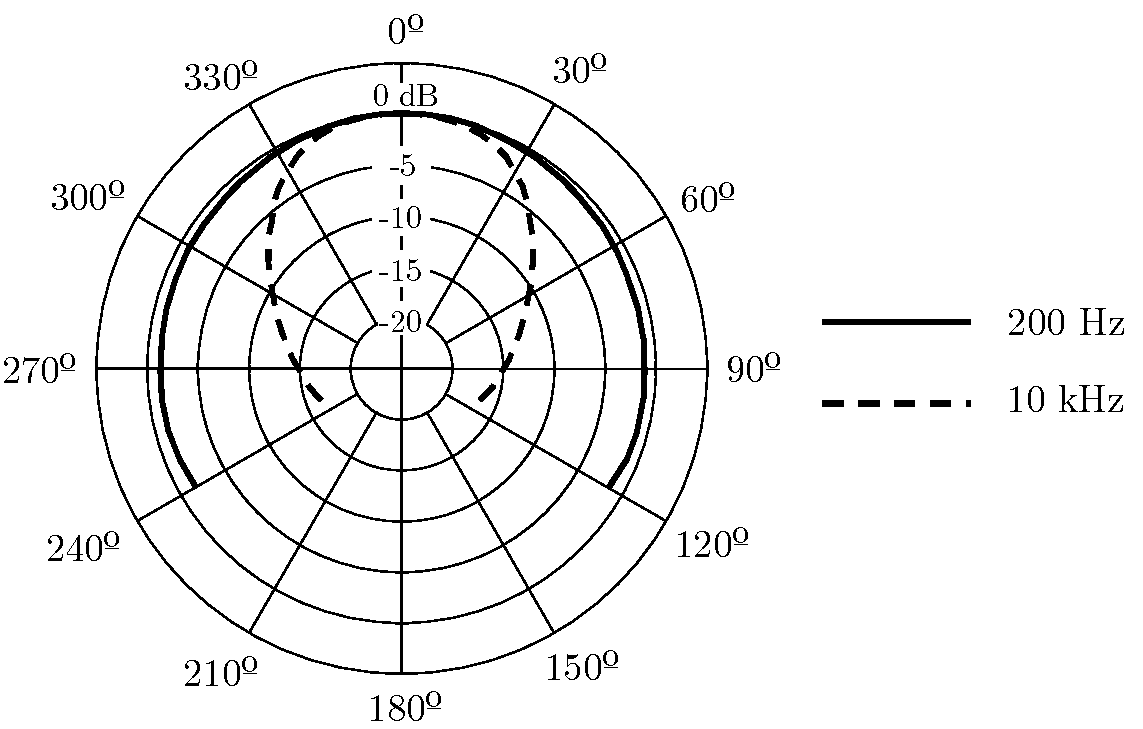
\includegraphics[width=0.6\textwidth]{archivos/diagramadirectividad.pdf}
    \caption{Diagrama de directividad de un altavoz de dos vías. Se representa la directividad emitiendo dos frecuencias diferentes.}
    \label{fig:directividad}
\end{figure}

\subsection{Factor e índice de directividad}
\label{directividad}
En ocasiones es útil tener un único valor, \textit{factor de directividad} o $Q$, que represente la directividad que tiene una fuente, sobretodo en cálculos donde se tenga en cuenta la directividad de la fuente pero no sea relevante el nivel en cada ángulo de emisión.
Este valor es la relación entre la intensidad acústica (\ref{intensidadacustica}) emitida en la dirección de máxima emisión y la que emitiría una fuente isótropa (omnidireccional) a igual potencia acústica.

\begin{flalign*}
	Q_0 = \frac{I(\theta_0,\Psi_0)}{I_{ISO}}
\end{flalign*}

La mayoría de ocasiones, la directividad no es homogénea como sí lo es en la figura \ref{fig:directividad} y para calcular un único valor hay que integrar los valores de intensidad en los diferentes ángulos de emisión:

\begin{flalign*}
	Q = \frac{4\pi I(\theta_0,\Psi_0)}{\bigintss_{\;0}^{2\pi} \bigintss_{\; 0}^{\pi} \sin (\theta) I(\theta,\Psi) \mathrm{d}\Psi \mathrm{d}\theta}
\end{flalign*}

Que teniendo en cuenta la simetría de revolución y desarrollando, el cálculo del factor de directividad se obtiene mediante:

\begin{flalign}
	Q = \frac{2}{\sum\limits_{i=1}^n \frac{I(\theta_i)}{I(\theta_0)}\sin (\theta_i) \Delta\theta_i}
\end{flalign}
\begin{condiciones}[Donde:]
	I(\theta_0) & \rightarrow & Es la intensidad en la dirección de máxima emisión.\\
	n & \rightarrow & Es el número de ángulos donde se tiene el valor de la intensidad.\\
	\Delta\theta & \rightarrow & Es la distancia en grados entre el ángulo $i$ y el ángulo $i+1$.
\end{condiciones}

En este trabajo se utilizará una fuente omnidireccional, por lo que tiene un factor de directividad $Q=1$, pero se debe tener en cuenta que esta directividad puede verse modificada por la posición de la fuente respecto al suelo, paredes o techo, tal como se muestra a continuación:

\begin{figure}[ht]
    \centering
    \begin{subfigure}[b]{0.3\textwidth}
    	\centering
        \includegraphics[width=0.5\linewidth]{archivos/Q1.png}
        \caption{$Q=1$.}
    \end{subfigure}
    ~ % Añadir el espacio deseado, si se deja la linea en blanco la siguiente subfigura ira en una nueva linea
    \begin{subfigure}[b]{0.3\textwidth}
    	\centering
        \includegraphics[width=0.8\linewidth]{archivos/Q2.png}
        \caption{$Q=2$.}
    \end{subfigure}
    
    \begin{subfigure}[b]{0.3\textwidth}
    	\centering
        \includegraphics[width=0.8\linewidth]{archivos/Q4.png}
        \caption{$Q=4$.}
    \end{subfigure}
    ~ % Añadir el espacio deseado, si se deja la linea en blanco la siguiente subfigura ira en una nueva linea
    \begin{subfigure}[b]{0.3\textwidth}
    	\centering
        \includegraphics[width=0.6\linewidth]{archivos/Q8.png}
        \caption{$Q=8$.}
    \end{subfigure}
    \caption{Modificación del factor de directividad producido por uno o varios planos.}\label{sistemass1}
\end{figure}

El índice de directividad determina cuántos decibelios aumenta la intensidad en el eje de máxima radiación respecto a una fuente omnidireccional, se calcula:

\begin{flalign}
	DI = 10\log_{10} Q
\end{flalign}
\subsection{Potencia acústica}

La potencia acústica, representada por la letra $W$, describe la energía por unidad de tiempo que emite una fuente acústica. Es un valor intrínseco de cada fuente, es decir, no depende de las condiciones físicas del medio o la distancia, se mantiene constante.
Las unidades de este parámetro son los vatios ($W$) o los julios por segundo ($J/s$).

\subsection{Intensidad acústica}
\label{intensidadacustica}

La intensidad acústica se define como la potencia acústica por unidad de superficie, se representa con la letra $I$ y sus unidades son los $W/m^2$.

\begin{flalign}
	I = \frac{W}{S}
\end{flalign}

\subsection{Presión acústica}
Es la variación de presión local sobre la presión absoluta o atmosférica producida por las ondas acústicas, se representa con la letra $p$ y sus unidades son los pascales. La suma neta resultante es igual a la presión absoluta.

Utilizando un símil sencillo como es un muelle se pueden comprender estas variaciones locales de presión:

\begin{figure}[ht]
    \centering
    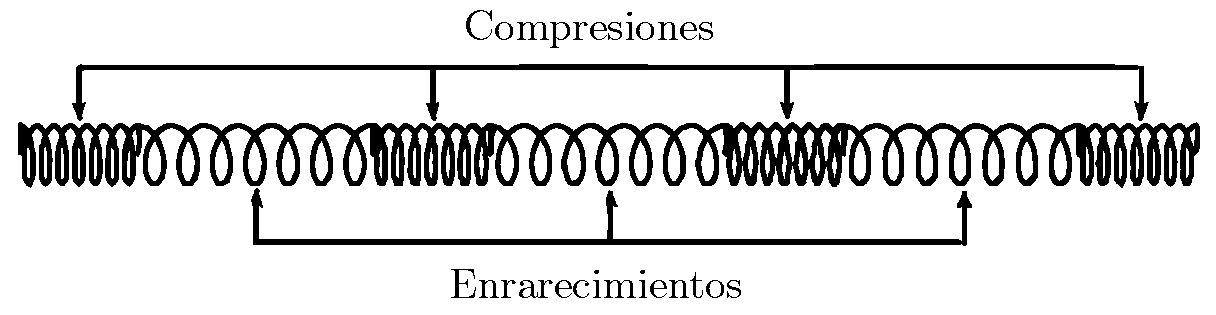
\includegraphics[width=0.6\textwidth]{archivos/presion.pdf}
    \caption{Compresión y enrarecimiento de un muelle como ejemplo de la variación de presión producida por ondas acústicas.}
\end{figure}

\subsection{Divergencia esférica}

Éste es un concepto físico necesario para comprender cómo evoluciona la intensidad acústica (\ref{intensidadacustica}) emitida por una fuente omnidireccional. La divergencia esférica describe cómo se distribuye la energía acústica emitida omnidireccionalmente en el espacio.

Una fuente acústica omnidireccional emite uniformemente intensidad en todas las direcciones, es decir, se propaga esféricamente. Según transcurre el tiempo la intensidad recorre más distancia y la esfera aumenta de tamaño distribuyendo la intensidad en una superficie aún mayor, esto se puede calcular como:

\begin{flalign}
	I = \frac{W}{S}
\end{flalign}
\begin{condiciones}[Donde:]
	W & \rightarrow & Es la potencia acústica de la fuente en vatios.\\
	I & \rightarrow & Es la intensidad recibida a una distancia $r$ en metros.\\
	S & = & $4\pi r^2$, es la superficie de una esfera de radio $r$.
\end{condiciones}


\begin{figure}[ht]
    \centering
    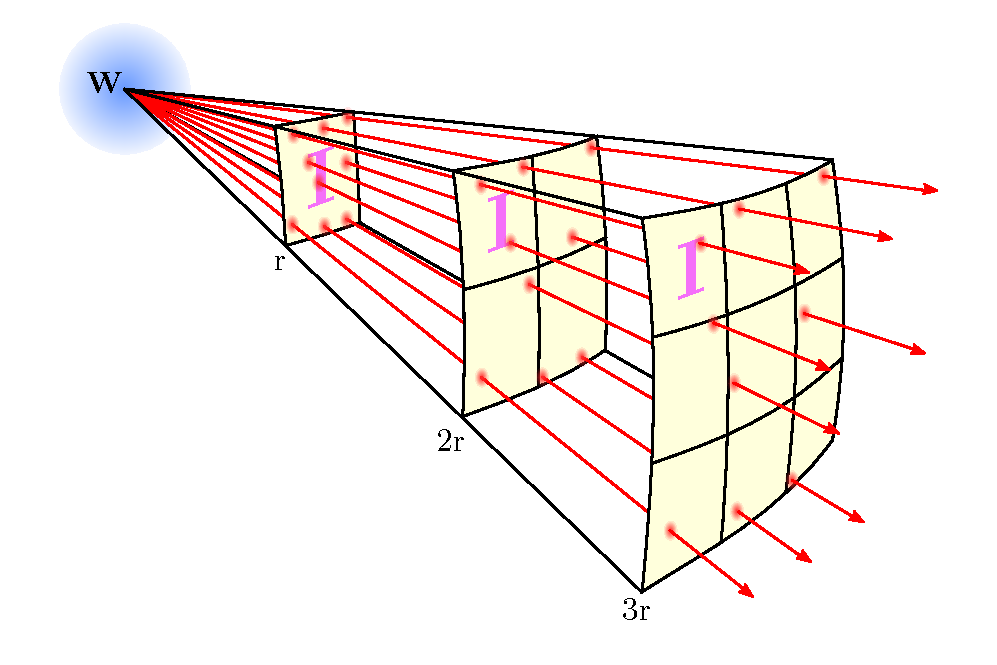
\includegraphics[width=0.6\textwidth]{archivos/divergenciaesferica.pdf}
    \caption{Representación gráfica de la divergencia esférica respecto a la distancia. Autor de la figura original: \textit{Borb}, de Wikipedia.}
\end{figure}

Si se tiene el valor de la intensidad a una distancia $r_1$ y se desea conocer el valor de intensidad a una distancia $r_2$ de la primera se puede utilizar lo que se denomina \textit{ley de la inversa del cuadrado de la distancia} que no es más que una derivación de la ecuación de la divergencia esférica.

\begin{flalign}
	I_2 = \frac{r_1^2}{r_2^2}I_1
\end{flalign}

Si la fuente tiene factor de directividad distinto a 1 (omnidireccional) se puede calcular la intensidad incluyendo el factor:

\begin{flalign}
	I = \frac{WQ}{S}
\end{flalign}
\begin{condiciones}[Donde:]
		Q & \rightarrow & Es el factor de directividad de la fuente.
\end{condiciones}

\subsection{Divergencia cilíndrica}

El concepto es el mismo que el de la divergencia esférica pero en este caso la intensidad en lugar de propagarse sobre la superficie de una esfera lo hace sobre la superficie lateral de un cilindro. Este tipo de divergencia se obtiene con fuentes lineales aunque mediante guías de ondas o alineando varias fuentes es posible modificar un frente de ondas de esférico a cilíndrico.

\begin{figure}[ht]
    \centering
    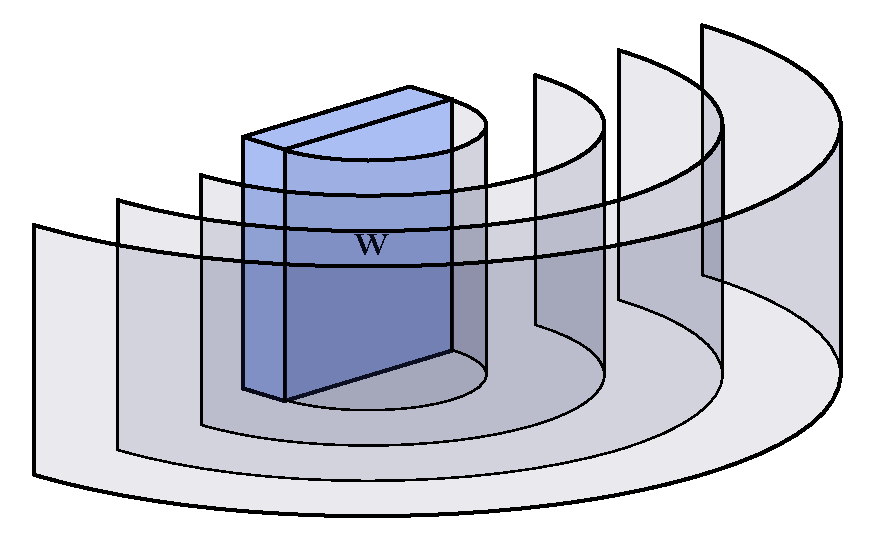
\includegraphics[width=0.6\textwidth]{archivos/divergenciacilindrica.pdf}
    \caption{Representación gráfica de la divergencia cilíndrica respecto a la distancia.}
\end{figure}
\FloatBarrier

El cálculo es el mismo que con la divergencia esférica pero teniendo en cuenta que ahora el área es el de un cilindro:

\begin{flalign}
	I = \frac{W}{S}
\end{flalign}
\begin{condiciones}[Donde:]
	S & = & $2\pi rh$, es la superficie de un cilindro de radio $r$ y altura $h$.
\end{condiciones}


\subsection{Densidad del aire}

Una densidad es la relación entre la mása y el volumen, se representa con la letra $\rho$ y sus unidades son los $Kg/m^3$. Para el caso del aire se puede calcular de forma simplificada como:

\begin{flalign}
	\rho = \frac{p}{R_{específica}T}
\end{flalign}
\begin{condiciones}[Donde:]
	p & \rightarrow & Es la presión atmosférica en pascales, 101.325 kPa.\\
	R_{específica} & \rightarrow & Es la constante específica del aire en $J\cdot(kg\cdot K)^{-1}$, para el aire seco $R_{específica}=287.058$.\\
	T & \rightarrow & Es la temperatura en kelvin. $T = 273.15 +\; ^{\circ}C$.
\end{condiciones}

\subsection{Velocidad del sonido en el aire}
La velocidad del sonido se representa con la letra $c$ y sus unidades son los $m/s$. Esta velocidad depende de la temperatura, la presión y la humedad, pero simplificando se puede calcular como:

\begin{flalign}
	c = \sqrt{\frac{\gamma RT}{M}}
\end{flalign}
\begin{condiciones}[Donde:]
	\gamma & \rightarrow & Es el coeficiente de dilatación adiabática del aire, para el aire seco $\gamma=1.4$.\\
	R & \rightarrow & Es la constante universal de los gases, $8.314\; J/(mol\cdot K)$.\\
	T & \rightarrow & Es la temperatura en kelvin. $T = 273.15 +\; ^{\circ}C$.\\
	M & \rightarrow & Es la mása molar del aire, $0.029\; kg/mol$.
\end{condiciones}

\subsection{Impedancia acústica específica del aire}

La impedancia acústica específica del aire es la oposición al flujo de energía acústica del aire, se representa con la letra $Z$ y sus unidades son $Pa\cdot s/m$ o $rayl$\footnote{La unidad $rayl$ se llama así en honor al físico John William Strutt, también conocido como Lord Rayleigh o John Rayleigh.}.

Esta impedancia se calcula mediante la densidad del aire $\rho$ y la velocidad del sonido $c$. 
\begin{flalign}
	Z = \rho c
\end{flalign}


\subsection{Escala logarítmica}

Los valores de presión, potencia o intensidad acústica sufren grandes variaciones por lo que para trabajar con ellos fácilmente se recurre a la escala logarítmica, a continuación se muestra la conversión de lineal a escala logarítmica de la presión, potencia e intensidad acústica, todos ellos son adimensionales y sus unidades son los decibelios o $dB$.

\begin{flalign}
	L_p =& 10\log_{10}\left(\frac{p_{ef}^2}{p_0^2}\right)=20\log_{10}\left(\frac{p_{ef}}{p_0}\right)\label{eq:nivelpresion} \\
	L_W =& 10\log_{10}\left(\frac{W}{W_0}\right)\\
	L_I =& 10\log_{10}\left(\frac{I}{I_0}\right)
\end{flalign}
\begin{condiciones}[Donde:]
	p_0 & \rightarrow & Es la presión de referencia, $2\cdot10^{-5}\;Pa$.\\
	W_0 & \rightarrow & Es la potencia de referencia, $1\;pW$ o $10^{-12}\;W$.\\
	I_0 & \rightarrow & Es la intensidad de referencia, $10^{-12}\;W/m^2$.
\end{condiciones}

El nivel de presión acústica $L_p$ también se suele nombrar como SPL (\textit{sound pressure level}) y el nivel de potencia como SWL.

De igual modo, si se tienen estos valores en escala logarítmica y se quiere trabajar con ellos en escala lineal, la conversión es la siguiente\footnote{Es una simple resolución matemática pero debido a múltiples errores encontrados en la literatura se ha decidido desarrollarlo.}:

\begin{flalign}
	p =& 10^{\frac{L_p}{20}}p_0\\
	W =& 10^{\frac{L_W}{10}}W_0 \\
	I =& 10^{\frac{L_I}{10}}I_0
\end{flalign}

\subsection{Relación entre presión y potencia o intensidad acústica}

Teniendo en cuenta ciertos parámetros se puede relacionar fácilmente el concepto de potencia, intensidad y presión acústica.

Si se conoce la presión acústica a una distancia $r$ de la fuente, la potencia acústica resultante será:

\begin{flalign}
	W = \frac{p_{ef}^24\pi r^2}{Z}
\end{flalign}
\begin{condiciones}[Donde:]
	p_{ef} & \rightarrow & Es la presión acústica eficaz, es la que mide cualquier sonómetro.
\end{condiciones}

Siguiendo el caso en el que se conoce la presión acústica, se puede calcular la intensidad acústica con:

\begin{flalign}\label{eq:intensidadimpedancia}
	I = \frac{p_{ef}^2}{Z}
\end{flalign}

Para los casos en los que se esté trabajando en escala logarítmica los cálculos para la potencia son:

\begin{flalign}
	L_W =& L_p + 10\log_{10}\left(\frac{4\pi r^2}{Q}\right)\\
	L_W \approx & L_p + 20\log_{10}r + 11\; ;\quad \mathrm{sí }\quad Q =1
\end{flalign}

\subsection{Bandas de frecuencia}

Las bandas de frecuencia son las fracciones en las que se divide el espectro audible (mínimo entre 20 Hz y 20000 Hz) de un sonido, se caracterizan por tener una frecuencia límite inferior $f_i$, otra superior $f_s$ y una central $f_c$. El punto de referencia para el cálculo del resto de frecuencias es la frecuencia central de 1000 Hz.

Las bandas de frecuencia en el espectro audible más habituales son la denominadas bandas de octava, entre una frecuencia central y la siguiente la relación es el doble y la relación entre sus límites y central es:
$$f_c = \sqrt{2}f_i$$
$$f_s = 2f_i$$
Otras bandas de frecuencia habituales son los tercios de octava donde las relaciones entre frecuencias centrales cumplen $2^{1/3}$, por lo que se puede observar que tres tercios dan como resultado una octava. Sus relaciones son las siguientes:
$$f_c=\sqrt[6]{2}f_i$$
$$ f_s = \sqrt[3]{2}f_i$$

\begin{table}[ht]
\centering
{\scalefont{0.9}
\begin{tabular}{@{}cccccccccc@{}}
\toprule
\multicolumn{10}{c}{Bandas de octava (Hz)}                      \\ \midrule
31.5 & 63 & 125 & 250 & 500 & 1000 & 2000 & 4000 & 8000 & 16000 \\ \bottomrule
\end{tabular}
}
\caption{Frecuencias centrales para las bandas de octava más utilizadas (ISO 266:1997).}
\end{table}

Se han desarrollado unas líneas de código Matlab para crear fácilmente cualquier fracción de bandas de frecuencia (octava: $n=1$, tercios de octava $n=3$, sextos de octava $n=6$, etc):

\begin{lstlisting}[style=Matlab-color,numbers=none, caption={Función Matlab para obtener cualquier fracción $n$ de bandas de frecuencia del espectro audible.},label=octavas]
FrecCentral = 10^3 * (2 .^ ((-6*n:4*n+n/3)/n)); % Vector de frecuencias centrales 1/n octavas
FrecDist = 2^(1/(2*n)); % Distancia entre central y corte superior o inferior
FrecSup = FrecCentral .* FrecDist; % Frecuencias límite superior
FrecInf = FrecCentral ./ FrecDist; % Frecuencias límite inferior
\end{lstlisting}


\subsection{Ponderación A}

El oído humano no percibe todas las frecuencias por igual tal como demostraron \cite{Fletcher1933}, por ello es necesario ponderar el nivel de presión de cada banda de frecuencia (octavas, tercios de octava, ...) para representar correctamente cómo lo percibirá el oído humano. La ponderación A corresponde a la inversa de la  curva de 40 fons de las curvas Fletcher-Munson.

Existen múltiples tablas en la literatura que definen el valor de corrección para cada banda de frecuencia, pero es preferible utilizar la función (obtenida mediante regresión y establecida en IEC 61672-1:2013) con la que se obtienen estos valores para cualquier frecuencia $f$:

\begin{flalign}
	A (f)= 20\log_{10}\left( \frac{12194^2f^4}{(f^2+20.6^2)\sqrt{(f^2+107.7^2)(f^2+737.9^2}\;(f^2+12194^2)} \right) + 2.0
\end{flalign}

La ponderación se aplica sumando esta al nivel de presión de la banda de frecuencia $f$.

\subsection{Suma de niveles}

En ocasiones es necesario sumar los niveles en decibelios de varias fuentes o sumar el nivel obtenido en lineal para pasarlo a bandas de octava, tercios de octava o a nivel global, para ello la suma se realiza del siguiente modo:

\begin{flalign}
	L_{sum} = 10\log_{10}\left( 10^{\nicefrac{L_1}{10}} + 10^{\nicefrac{L_2}{10}} + ... + 10^{\nicefrac{L_n}{10}}\right)
\end{flalign}
\begin{condiciones}[Donde:]
	L_1, L_2, L_n & \rightarrow & Son los n niveles en dB a sumar.
\end{condiciones}

Por ejemplo, para el paso de tercios de octava a bandas de octava la suma para obtener el valor en la banda de octava de 125 Hz será:

\begin{flalign*}
	L_{125\text{Hz}} = 10\log_{10}\left( 10^{\nicefrac{L_{100\text{Hz}}}{10}} + 10^{\nicefrac{L_{125\text{Hz}}}{10}} + 10^{\nicefrac{L_{160\text{Hz}}}{10}} \right)
\end{flalign*}

\subsection{Ruido rosa/blanco}
\label{ruidos}
En la mayoría de mediciones para conocer principalmente la respuesta en frecuencia de los elementos de emisión, captación o recintos, se emiten señales como el ruido blanco o el ruido rosa.
\\
\par
El ruido blanco se caracteriza por ser una señal con el mismo nivel en todas las frecuencias produciendo, cuando se traslada a bandas de octava, que haya un incremento de 3dB por octava dado que cada octava tiene el doble de ancho de banda que la anterior y por tanto se suma el doble de energía ($10\log_{10}(2)=3 dB$).

\begin{figure}[ht]
    \centering
    {\scalefont{0.8}
    %%%%%%%%%%%%%%%%%%%%%%%%%%%%%%%%%%%%%%%%%%%%%%%%%%%%%%%%%%%%%%%%%%%%%%%%
% Escuela Politécnica Superior de la Universidad de Alicante
% Realizado por: Jose Manuel Requena Plens
% Contacto: info@jmrplens.com / Telegram:@jmrplens
%%%%%%%%%%%%%%%%%%%%%%%%%%%%%%%%%%%%%%%%%%%%%%%%%%%%%%%%%%%%%%%%%%%%%%%%

\definecolor{mycolor1}{rgb}{0.00000,0.44700,0.74100}%
%
\begin{tikzpicture}

\begin{axis}[%
width=0.5\textwidth,
height=0.35\textwidth,
at={(0\textwidth,0\textwidth)},
scale only axis,
area style,
stack plots=y,
xmode=log,
xmin=11.5,
xmax=12000,
grid=major,
xtick={16.62,31.25,62.5,125,250,500,1000,2000,4000,8000,16000},
xticklabels={{16},{31.25},{62.5},{125},{250},{500},{1000},{2000},{4000},{8000},{16000}},
xminorticks=true,
xlabel style={font=\color{white!15!black}},
xlabel={Frecuencia (Hz)},
ymin=0,
ymax=50,
ylabel style={font=\color{white!15!black}},
ylabel={Nivel (dB)},
axis background/.style={fill=white},
legend style={at={(0.03,0.97)}, anchor=north west, legend cell align=left, align=left, draw=white!15!black}
]
\draw[line width=1.5pt,  pattern=north west lines, pattern color=orange] (axis cs:12.0485434560398,-10) rectangle (axis cs:22.0970869120796,20.7918124604762);
\draw[line width=1.5pt,  pattern=north west lines, pattern color=orange] (axis cs:22.0970869120796,-10) rectangle (axis cs:44.1941738241592,23.6172783601759);
\draw[line width=1.5pt,  pattern=north west lines, pattern color=orange] (axis cs:44.1941738241592,-10) rectangle (axis cs:88.3883476483184,26.5321251377534);
\draw[line width=1.5pt, pattern=north west lines, pattern color=orange] (axis cs:88.3883476483184,-10) rectangle (axis cs:176.776695296637,29.4939000664491);
\draw[line width=1.5pt,  pattern=north west lines, pattern color=orange] (axis cs:176.776695296637,-10) rectangle (axis cs:353.553390593274,32.5042000230889);
\draw[line width=1.5pt,  pattern=north west lines, pattern color=orange] (axis cs:353.553390593274,-10) rectangle (axis cs:707.106781186548,35.5022835305509);
\draw[line width=1.5pt,  pattern=north west lines, pattern color=orange] (axis cs:707.106781186547,-10) rectangle (axis cs:1414.2135623731,38.5003325768977);
\draw[line width=1.5pt,  pattern=north west lines, pattern color=orange] (axis cs:1414.21356237309,-10) rectangle (axis cs:2828.42712474619,41.5075643986031);
\draw[line width=1.5pt,  pattern=north west lines, pattern color=orange] (axis cs:2828.42712474619,-10) rectangle (axis cs:5656.85424949238,44.5163294745699);
\draw[line width=1.5pt,  pattern=north west lines, pattern color=orange] (axis cs:5656.85424949238,-10) rectangle (axis cs:11313.7084989848,47.5266294312097);
\addlegendimage{line width=1.5pt,  pattern=north west lines, pattern color=orange}
\addlegendentry{Ruido blanco - octavas}

\addplot[fill=mycolor1, draw=black] table[row sep=crcr]{%
1	20\\
16000	20\\
}
\closedcycle;
\addlegendentry{Ruido blanco - lineal}

\end{axis}
\end{tikzpicture}%
    }
    \caption{Representación de ruido blanco tanto en lineal como por octavas.}
    \label{graf:ruidoblanco}
\end{figure}
\FloatBarrier
El ruido rosa corrige el efecto producido en el ruido blanco, introduciendo una atenuación de 3dB por octava, es por ello por lo que es el ruido más habitual en mediciones que se analizan por bandas de octava, ya que mantiene el mismo valor de energía en todas las bandas de octava.

\begin{figure}[ht]
    \centering
    {\scalefont{0.8}
    %%%%%%%%%%%%%%%%%%%%%%%%%%%%%%%%%%%%%%%%%%%%%%%%%%%%%%%%%%%%%%%%%%%%%%%%
% Plantilla TFG/TFM
% Escuela Politécnica Superior de la Universidad de Alicante
% Realizado por: Jose Manuel Requena Plens
% Contacto: info@jmrplens.com / Telegram:@jmrplens
%%%%%%%%%%%%%%%%%%%%%%%%%%%%%%%%%%%%%%%%%%%%%%%%%%%%%%%%%%%%%%%%%%%%%%%%

\definecolor{mycolor1}{rgb}{0.00000,0.44700,0.74100}%
%
\begin{tikzpicture}

\begin{axis}[%
width=0.5\textwidth,
height=0.35\textwidth,
at={(0\textwidth,0\textwidth)},
scale only axis,
area style,
stack plots=y,
xmode=log,
xmin=11.5,
xmax=12000,
grid=major,
xtick={16.62,31.25,62.5,125,250,500,1000,2000,4000,8000,16000},
xticklabels={{16},{31.25},{62.5},{125},{250},{500},{1000},{2000},{4000},{8000},{16000}},
xminorticks=true,
xlabel style={font=\color{white!15!black}},
xlabel={Frecuencia (Hz)},
ymin=0,
ymax=50,
ylabel style={font=\color{white!15!black}},
ylabel={Nivel (dB)},
axis background/.style={fill=white},
legend style={at={(0.03,0.97)}, anchor=north west, legend cell align=left, align=left, draw=white!15!black}
]
\draw[line width=1.5pt,  pattern=north west lines, pattern color=orange] (axis cs:12.0485434560398,-10) rectangle (axis cs:22.0970869120796,38.5395005764647);
\draw[line width=1.5pt,  pattern=north west lines, pattern color=orange] (axis cs:22.0970869120796,-10) rectangle (axis cs:44.1941738241592,38.4765584900126);
\draw[line width=1.5pt,  pattern=north west lines, pattern color=orange] (axis cs:44.1941738241592,-10) rectangle (axis cs:88.3883476483184,38.4431162668429);
\draw[line width=1.5pt,  pattern=north west lines, pattern color=orange] (axis cs:88.3883476483184,-10) rectangle (axis cs:176.776695296637,38.4258681272424);
\draw[line width=1.5pt,  pattern=north west lines, pattern color=orange] (axis cs:176.776695296637,-10) rectangle (axis cs:353.553390593274,38.4347351341331);
\draw[line width=1.5pt,  pattern=north west lines, pattern color=orange] (axis cs:353.553390593274,-10) rectangle (axis cs:707.106781186548,38.4215119396158);
\draw[line width=1.5pt,  pattern=north west lines, pattern color=orange] (axis cs:707.106781186547,-10) rectangle (axis cs:1414.2135623731,38.4104672378742);
\draw[line width=1.5pt,  pattern=north west lines, pattern color=orange] (axis cs:1414.21356237309,-10) rectangle (axis cs:2828.42712474619,38.4093616516654);
\draw[line width=1.5pt,  pattern=north west lines, pattern color=orange] (axis cs:2828.42712474619,-10) rectangle (axis cs:5656.85424949238,38.4088083131028);
\draw[line width=1.5pt,  pattern=north west lines, pattern color=orange] (axis cs:5656.85424949238,-10) rectangle (axis cs:11313.7084989848,38.4090852235989);
\addlegendimage{line width=1.5pt,  pattern=north west lines, pattern color=orange}
\addlegendentry{Ruido rosa - octavas}

\addplot[fill=mycolor1, draw=black] table[row sep=crcr]{%
1	50\\
16000	7.95880017344075\\
}
\closedcycle;
\addlegendentry{Ruido rosa - lineal}

\end{axis}
\end{tikzpicture}%
    }
    \caption{Representación de ruido rosa tanto en lineal como por octavas.}
    \label{graf:ruidorosa}
\end{figure}
\FloatBarrier


\subsection{Nivel continuo equivalente}

El nivel continuo equivalente es la media energética del nivel de un ruido o sonido promediado en el tiempo, es básicamente un nivel promedio de una medida contínua. Debido a la alta variabilidad de nivel de un sonido no es correcto escoger un valor de un instante concreto, se debe obtener un promedio de todos los valores instantáneos obtenidos. 

Este nivel se puede calcular como:

\begin{flalign}
	L_{eq} = 10\log_{10}\left( \frac{1}{T} \bigintsss_0^{T}\left( \frac{p^2(t)}{p^2_0} \right)\text{d}t \right)
\end{flalign}
\begin{condiciones}[Donde:]
	p^2(t) & \rightarrow & Son los valores instantáneos de presión al cuadrado.\\
	T & \rightarrow & Es la duración de la medida.
\end{condiciones}

Para entenderlo fácilmente se muestra en la figura \ref{graf:leq} una señal captada y su valor $L_{eq}$.

\begin{figure}[ht]
    \centering
    {\scalefont{0.8}
    %%%%%%%%%%%%%%%%%%%%%%%%%%%%%%%%%%%%%%%%%%%%%%%%%%%%%%%%%%%%%%%%%%%%%%%%
% Escuela Politécnica Superior de la Universidad de Alicante
% Realizado por: Jose Manuel Requena Plens
% Contacto: info@jmrplens.com / Telegram:@jmrplens
%%%%%%%%%%%%%%%%%%%%%%%%%%%%%%%%%%%%%%%%%%%%%%%%%%%%%%%%%%%%%%%%%%%%%%%%

\definecolor{mycolor1}{rgb}{0.00000,0.44700,0.74100}%
\definecolor{mycolor2}{rgb}{0.85000,0.32500,0.09800}%
%
\begin{tikzpicture}

\begin{axis}[%
width=0.5\textwidth,
height=0.22\textwidth,
at={(0\textwidth,0\textwidth)},
scale only axis,
xmin=0,
xmax=1,
xlabel style={font=\color{white!15!black}},
xlabel={Tiempo (s)},
ymin=44,
ymax=58,
ylabel style={font=\color{white!15!black}},
ylabel={Nivel (dB)},
axis background/.style={fill=white},
legend style={legend cell align=left, align=left, draw=white!15!black}
]
\addplot [color=mycolor1, line width=1.5pt]
  table[row sep=crcr]{%
0	50\\
0.00598412698412432	52.4354905344046\\
0.00923265306122545	53.5863011944272\\
0.0117972789115655	54.3566439459881\\
0.0140199546485249	54.9087296789833\\
0.0160716553288012	55.3167194619479\\
0.0177814058956898	55.5811991715484\\
0.0193201814058952	55.761725842872\\
0.0206879818594103	55.8783677034787\\
0.0218848072562352	55.94850013745\\
0.0229106575963698	55.9864430085202\\
0.0237655328798212	56.0035077107261\\
0.0242784580498849	56.0077962188932\\
0.0246204081632655	56.0083021094971\\
0.0249623582766461	56.006998772416\\
0.0254752834467098	56.0017924852514\\
0.0261591836734709	55.9891287470019\\
0.0270140589569152	55.964866713046\\
0.0282108843537401	55.917113228018\\
0.0297496598639455	55.8365743707716\\
0.031972335600905	55.6946034737216\\
0.0382984126984098	55.2754066432793\\
0.0401791383219958	55.1830307099835\\
0.0417179138322012	55.1265260868083\\
0.0429147392290261	55.0956856199849\\
0.0439405895691607	55.0787261109273\\
0.044795464852605	55.0713075112947\\
0.0453083900226758	55.0697543991762\\
0.0456503401360564	55.0699075357098\\
0.0459922902494299	55.0709970048091\\
0.0465052154195007	55.0743537532379\\
0.0471891156462618	55.0819503877214\\
0.0480439909297061	55.0962202298286\\
0.049240816326531	55.1243828267478\\
0.0507795918367364	55.172654131706\\
0.0528312925170056	55.2526687159606\\
0.059499319727891	55.5270521762376\\
0.0610380952380964	55.5691566346894\\
0.0622349206349213	55.5912047631082\\
0.0630897959183656	55.6003790190219\\
0.0636027210884365	55.6030481201545\\
0.063944671201817	55.6035964552583\\
0.0642866213151905	55.6031352708759\\
0.0647995464852613	55.6005094439748\\
0.0654834467120153	55.5933129193599\\
0.0663383219954667	55.5782339045611\\
0.0673641723356013	55.5510446711095\\
0.0685609977324262	55.5066901016045\\
0.0699287981859413	55.4395422431632\\
0.071638548752837	55.3320164838049\\
0.0736902494331062	55.1717762067451\\
0.0762548752834462	54.9330280877809\\
0.0803582766439916	54.5022082506331\\
0.0846326530612274	54.0657081040926\\
0.0871972789115674	53.8463091484114\\
0.0892489795918365	53.7068243121441\\
0.0909587301587322	53.6193736597434\\
0.0923265306122474	53.5695720913139\\
0.0935233560090722	53.540957576204\\
0.0943782312925165	53.5289806251965\\
0.0950621315192777	53.5243535395645\\
0.0954040816326511	53.5236495705989\\
0.0957460317460317	53.523993553022\\
0.0960879818594123	53.5253639467535\\
0.096600907029476	53.5292916732686\\
0.0972848072562371	53.5378824132796\\
0.0983106575963717	53.5574570349797\\
0.0995074829931966	53.589293956492\\
0.101217233560092	53.6482056726565\\
0.103952834467123	53.7613545296413\\
0.107030385487526	53.8852252003745\\
0.108569160997732	53.9329238430555\\
0.109765986394557	53.9587877425379\\
0.110620861678008	53.9697707860655\\
0.111133786848072	53.9729655370425\\
0.111475736961452	53.9735754401465\\
0.111646712018143	53.9734061680292\\
0.111988662131516	53.9720897026781\\
0.112501587301587	53.9675847530432\\
0.113185487528348	53.9566267982607\\
0.114040362811792	53.9345181675708\\
0.115066213151927	53.894909844778\\
0.116263038548752	53.8296391955825\\
0.117630839002267	53.7287143078679\\
0.119169614512472	53.58056254502\\
0.120879365079368	53.3726807435709\\
0.122931065759637	53.0648349692087\\
0.125324716553287	52.63195704156\\
0.128231292517007	52.0188965665263\\
0.132676643990926	50.9728098492146\\
0.137976870748297	49.7464071698251\\
0.140883446712017	49.1734960804138\\
0.143106122448977	48.8130669029894\\
0.144986848072563	48.5704555848487\\
0.146696598639458	48.4035903571865\\
0.148064399092974	48.3080352645967\\
0.149261224489798	48.2520817101192\\
0.150116099773243	48.2276446720638\\
0.150799999999997	48.2171783741505\\
0.151312925170068	48.2144898852167\\
0.151654875283448	48.2150973258981\\
0.151996825396829	48.2175842741123\\
0.152509750566892	48.2247561656879\\
0.153193650793654	48.2405265016715\\
0.154219501133788	48.276742309395\\
0.155416326530613	48.3363917765509\\
0.156955102040818	48.4367998851375\\
0.159006802721088	48.6026366734534\\
0.162597278911562	48.937167690639\\
0.166016780045354	49.2404358226117\\
0.168068480725623	49.3849724235891\\
0.169607256235828	49.4649640458562\\
0.170804081632653	49.5070335294376\\
0.171658956916097	49.5252080414222\\
0.172342857142858	49.5322221102209\\
0.172684807256239	49.5331452722564\\
0.172855782312922	49.5329506885399\\
0.173197732426303	49.5312365786132\\
0.173710657596374	49.5253204908182\\
0.174394557823128	49.5111159593275\\
0.175249433106579	49.483109792913\\
0.176275283446714	49.4344202386435\\
0.177472108843538	49.3570110485449\\
0.179010884353744	49.2258792677841\\
0.180720634920633	49.0411581327237\\
0.182772335600909	48.7717738247189\\
0.185507936507939	48.3497047093896\\
0.190808163265309	47.4425225114763\\
0.194398639455784	46.8703030568826\\
0.196792290249434	46.553012272762\\
0.198673015873013	46.3541771017598\\
0.200211791383218	46.2297650090181\\
0.201579591836733	46.1503653509219\\
0.202605442176868	46.1107947731683\\
0.203460317460319	46.0910865112234\\
0.204144217687073	46.0840136411358\\
0.204486167800454	46.0833620008552\\
0.204828117913834	46.0846215078295\\
0.205341043083898	46.0900666070504\\
0.206024943310659	46.1038797536169\\
0.206879818594103	46.1314475355647\\
0.207905668934238	46.1791034408031\\
0.209273469387753	46.2659383951959\\
0.210812244897959	46.3925325489547\\
0.212863945578235	46.6016710673063\\
0.215428571428575	46.911107262663\\
0.225174149659864	48.1372865059723\\
0.227396825396823	48.3405936566567\\
0.229277551020409	48.4737618879328\\
0.230816326530615	48.5543515252333\\
0.23218412698413	48.60426633714\\
0.233209977324265	48.628518418714\\
0.234064852607709	48.6403827773358\\
0.23474875283447	48.6446246087346\\
0.235090702947844	48.6450587597203\\
0.235432653061224	48.6444028888133\\
0.235945578231295	48.6414369874469\\
0.236629478458049	48.6339422118275\\
0.237484353741493	48.6192557587475\\
0.238681179138325	48.5897827623002\\
0.240219954648524	48.5391188802128\\
0.2422716553288	48.4555773599565\\
0.249110657596368	48.1639985848597\\
0.250820408163264	48.1143188720163\\
0.252188208616779	48.0867152592828\\
0.253214058956914	48.0738836076406\\
0.253897959183675	48.0692604497106\\
0.254410884353739	48.0678971397999\\
0.254752834467119	48.067996395486\\
0.2550947845805	48.0689027747083\\
0.255607709750564	48.0717713382109\\
0.256291609977325	48.0783878528064\\
0.257146485260769	48.0910522002761\\
0.258343310657594	48.1166212829081\\
0.259711111111109	48.1561087345516\\
0.261420861678005	48.2184907175902\\
0.263985487528345	48.3306474956782\\
0.268943764172334	48.550836306189\\
0.27065351473923	48.6076300071772\\
0.272021315192745	48.6396405856957\\
0.27304716553288	48.6541251199986\\
0.273731065759634	48.6587063064382\\
0.274073015873014	48.6593772998538\\
0.274414965986395	48.6589292347146\\
0.274756916099776	48.6573347981512\\
0.275269841269839	48.6527384572647\\
0.2759537414966	48.6423758233884\\
0.276808616780045	48.6224026004332\\
0.277834467120179	48.5878426441998\\
0.279031292517004	48.532637077406\\
0.280399092970519	48.449880211023\\
0.282108843537415	48.3177497797406\\
0.284160544217684	48.1204170021778\\
0.286554195011341	47.845756358698\\
0.290315646258506	47.3559476209446\\
0.294760997732425	46.7877753004496\\
0.296983673469384	46.5541775598426\\
0.29869342403628	46.4142106774319\\
0.300061224489795	46.3332106651333\\
0.30108707482993	46.2929933244866\\
0.301941950113381	46.2740503553424\\
0.302454875283445	46.2693635437881\\
0.302625850340135	46.2689454472509\\
0.302796825396825	46.269107405271\\
0.303138775510206	46.2711894840592\\
0.30365170068027	46.2787711880909\\
0.304335600907031	46.2973620151626\\
0.305190476190475	46.334518530219\\
0.30621632653061	46.399910819006\\
0.307413151927435	46.5052549663249\\
0.30878095238095	46.664004062702\\
0.310490702947845	46.9189221564951\\
0.312371428571431	47.2683060542021\\
0.314594104308391	47.765356423519\\
0.317329705215421	48.4799196121116\\
0.321262131519276	49.6330463354924\\
0.327588208616781	51.4894805069492\\
0.330494784580502	52.212945761074\\
0.332717460317461	52.6703694875504\\
0.33459818594104	52.9804377590511\\
0.336307936507936	53.1957378105521\\
0.337675736961451	53.3205845693593\\
0.338872562358276	53.3949431139119\\
0.33989841269841	53.4329745181215\\
0.340582312925171	53.4453678042553\\
0.341095238095235	53.4479887278421\\
0.341266213151926	53.4476097420882\\
0.341608163265306	53.4449963716615\\
0.342121088435377	53.4365023546497\\
0.342804988662131	53.4168367832443\\
0.343659863945575	53.3793242941407\\
0.344856689342407	53.3040047470422\\
0.346224489795915	53.1880553022591\\
0.347934240362811	53.0040291488192\\
0.35015691609977	52.7129336136982\\
0.353405442176872	52.2207523753449\\
0.359902494331067	51.2247111677433\\
0.362467120181407	50.8992691556285\\
0.364689795918366	50.6688076687589\\
0.366570521541952	50.5153171133509\\
0.368280272108841	50.409439713517\\
0.369819047619046	50.3406767895916\\
0.371015873015871	50.3034653677367\\
0.372041723356013	50.2819760012005\\
0.372896598639457	50.2707546305028\\
0.373580498866211	50.2657537453453\\
0.374093424036282	50.2641208060775\\
0.374435374149662	50.2639649832585\\
0.374777324263036	50.2645068066611\\
0.375290249433107	50.2665342342228\\
0.375974149659861	50.2712756505498\\
0.377000000000002	50.2820289222041\\
0.378538775510201	50.3039141240853\\
0.382984126984127	50.3709522312875\\
0.384180952380952	50.3815574623752\\
0.385035827664396	50.385500008646\\
0.385548752834467	50.3861962210004\\
0.386061678004538	50.3855365450725\\
0.386574603174601	50.3834461558641\\
0.387258503401362	50.378321160959\\
0.388113378684807	50.3679805858118\\
0.389139229024941	50.3495661852696\\
0.390336054421766	50.3195982824875\\
0.391703854875281	50.2741900689585\\
0.393413605442177	50.2014697908492\\
0.395465306122446	50.0936395647225\\
0.398200907029477	49.924639021178\\
0.404356009070298	49.536699214932\\
0.406236734693877	49.4467700038023\\
0.407775510204083	49.3925586848454\\
0.408972335600907	49.364900465749\\
0.409827210884352	49.3538031947584\\
0.410340136054423	49.3508271227258\\
0.410682086167803	49.350430584747\\
0.411024036281177	49.3513306739522\\
0.411536961451247	49.3551567011862\\
0.412220861678001	49.364972866157\\
0.413075736961453	49.3849799238654\\
0.414101587301587	49.4205303853398\\
0.415298412698412	49.4780373692932\\
0.416666213151927	49.5646994201483\\
0.418375963718823	49.703258658712\\
0.420427664399092	49.9101042661913\\
0.422821315192742	50.1980158761141\\
0.426411791383217	50.690249916354\\
0.432053968253967	51.4635552694877\\
0.434447619047617	51.7346794397177\\
0.436328344671203	51.9056065570519\\
0.437867120181409	52.0123819766453\\
0.439234920634924	52.0797021025626\\
0.440260770975058	52.1122215959941\\
0.441115646258503	52.1272402122752\\
0.441628571428573	52.130928011669\\
0.441799546485264	52.131268197696\\
0.442141496598637	52.1306158242408\\
0.442483446712018	52.1281896413602\\
0.442996371882089	52.1212386464137\\
0.443680272108843	52.1058419437914\\
0.444535147392287	52.0769122564575\\
0.445731972789119	52.0189203754493\\
0.447099773242627	51.9290843910663\\
0.448809523809523	51.7849692405465\\
0.450861224489799	51.5732172898096\\
0.453767800453512	51.2240623052992\\
0.459922902494334	50.4703283324832\\
0.462145578231294	50.2543506674209\\
0.463855328798189	50.1261231124562\\
0.465223129251697	50.0518229035455\\
0.466248979591839	50.0142189143976\\
0.467103854875283	49.9953924628859\\
0.467787755102044	49.9887672400233\\
0.468129705215418	49.9883109830137\\
0.468471655328798	49.9897743779096\\
0.468984580498869	49.9955855307018\\
0.469668480725623	50.0101030660726\\
0.470523356009068	50.0391138479043\\
0.471549206349209	50.0896980211758\\
0.472746031746034	50.1699201687128\\
0.474284807256232	50.3049572033131\\
0.476165532879818	50.5142485356802\\
0.478388208616778	50.8139775001635\\
0.481465759637189	51.2928463979336\\
0.488133786848074	52.3486388470782\\
0.490527437641724	52.6520845620276\\
0.492408163265303	52.8385434311614\\
0.493946938775508	52.9508231326223\\
0.495143764172333	53.0107710067512\\
0.496169614512475	53.0421629034776\\
0.496853514739229	53.0526018187468\\
0.4973664399093	53.05487011966\\
0.49753741496599	53.0545640434276\\
0.497879365079363	53.0523580254946\\
0.498392290249434	53.0450689700267\\
0.499076190476188	53.027952845384\\
0.49993106575964	52.9947942604902\\
0.500956916099774	52.9381119954376\\
0.502324716553289	52.8349972378321\\
0.503863492063495	52.6839071287173\\
0.505744217687074	52.4545287261205\\
0.508137868480723	52.1052017089658\\
0.511728344671205	51.5069418352752\\
0.517370521541949	50.5672872676802\\
0.519935147392289	50.2100788965667\\
0.521986848072565	49.9776009592089\\
0.523696598639454	49.8261512326992\\
0.525235374149659	49.7251127208131\\
0.526432199546484	49.670192502367\\
0.527458049886619	49.6395560168582\\
0.52831292517007	49.625410638121\\
0.528825850340134	49.6217751106853\\
0.529167800453514	49.6213281488582\\
0.529509750566895	49.6224333152981\\
0.530022675736959	49.6269401729203\\
0.53070657596372	49.6381048777112\\
0.531561451247164	49.6599557597378\\
0.532758276643989	49.704179365035\\
0.534126077097504	49.7719526140995\\
0.53600680272109	49.8894092058847\\
0.53874240362812	50.0926115587059\\
0.5438716553288	50.4788091819886\\
0.545923356009069	50.6004090083252\\
0.547462131519275	50.669533089446\\
0.5486589569161	50.7077956811963\\
0.549684807256234	50.7287718498068\\
0.550368707482995	50.7363853157664\\
0.550881632653059	50.7386580054239\\
0.55122358276644	50.7385135252843\\
0.55156553287982	50.7370308202838\\
0.552078458049884	50.7322840027464\\
0.552762358276645	50.7212294283938\\
0.55361723356009	50.6998258396062\\
0.554643083900224	50.6631358290472\\
0.556010884353739	50.5960707540438\\
0.557549659863945	50.4972384582141\\
0.559430385487531	50.3462943871467\\
0.56182403628118	50.1149965871819\\
0.565243537414965	49.7359013076141\\
0.57156961451247	49.0300211336701\\
0.5743052154195	48.7769768772144\\
0.576527891156459	48.6095087255929\\
0.578408616780045	48.4971207786269\\
0.580118367346941	48.4181780393078\\
0.581657142857146	48.3648314359201\\
0.583195918367345	48.3263145062006\\
0.58456371882086	48.3024500322368\\
0.585931519274375	48.2860537150773\\
0.58729931972789	48.274609515022\\
0.590889795918365	48.2476529684\\
0.59208662131519	48.2329912860528\\
0.593283446712022	48.2123051726981\\
0.594480272108846	48.1838182418776\\
0.595848072562362	48.139639400629\\
0.59721587301587	48.0810653458654\\
0.598754648526075	47.9958905719435\\
0.600464399092971	47.8754270706891\\
0.602345124716557	47.7104509011004\\
0.604396825396826	47.4925991639393\\
0.606961451247166	47.1708802006225\\
0.61038095238095	46.6813337267971\\
0.616536054421772	45.7928854245008\\
0.618758730158731	45.5327510528766\\
0.620468480725627	45.3749011712117\\
0.621836281179135	45.2812998805456\\
0.623033106575967	45.2265281735582\\
0.623887981859411	45.2042480805085\\
0.624400907029475	45.197973727592\\
0.624742857142856	45.1968353899185\\
0.624913832199546	45.1971943224742\\
0.625255782312927	45.1997913566351\\
0.62576870748299	45.208448829887\\
0.626452607709751	45.2290426081555\\
0.627307482993196	45.2696218417695\\
0.62833333333333	45.3404790733952\\
0.629530158730162	45.4540870823845\\
0.63089795918367	45.6247942056414\\
0.632607709750566	45.8984680660475\\
0.634488435374152	46.2734134492314\\
0.636711111111111	46.8073639114754\\
0.639446712018142	47.577249707798\\
0.643208163265307	48.7720927974989\\
0.650731065759636	51.1907453865109\\
0.653637641723357	51.9762251330775\\
0.656031292517007	52.51125754424\\
0.658082993197276	52.8761320709283\\
0.659792743764172	53.1094388902131\\
0.661331519274377	53.2632185606873\\
0.662528344671202	53.3462538313218\\
0.663554195011336	53.3925289008781\\
0.664409070294788	53.4140656206961\\
0.664921995464852	53.4197885152271\\
0.665263945578232	53.4206835114855\\
0.665434920634922	53.4202704976919\\
0.665776870748303	53.4177508866453\\
0.666289795918367	53.4098241547757\\
0.666973696145128	53.3917706182272\\
0.667828571428572	53.3577668379464\\
0.669025396825397	53.2904118672348\\
0.670564172335602	53.1738746099437\\
0.672444897959181	52.994024986832\\
0.675009523809521	52.7027209355632\\
0.683216326530612	51.7366796832077\\
0.685439002267572	51.5380739337962\\
0.687319727891158	51.4057425210807\\
0.688858503401363	51.323562594087\\
0.690226303854878	51.2703612369956\\
0.691423129251703	51.238688913574\\
0.692448979591838	51.2220264317411\\
0.693132879818592	51.2159703430488\\
0.693645804988662	51.2139239781568\\
0.693987755102043	51.2136904959298\\
0.694329705215416	51.2143231939427\\
0.694842630385487	51.2168202212684\\
0.695526530612248	51.2228465810163\\
0.696552380952383	51.2370316813684\\
0.697920181405898	51.2637975661958\\
0.699800907029477	51.3104121550117\\
0.704246258503403	51.424162521376\\
0.705614058956918	51.4488813832181\\
0.706639909297053	51.4614957577408\\
0.707494784580497	51.4674222144642\\
0.708007709750568	51.4687796107775\\
0.708349659863948	51.4687166667667\\
0.708691609977322	51.4678534592661\\
0.709204535147393	51.4650144404349\\
0.709888435374147	51.4582551392232\\
0.710743310657598	51.4448683428718\\
0.711769160997733	51.4213637671291\\
0.712965986394558	51.3835432782633\\
0.714333786848073	51.3267390559043\\
0.716043537414969	51.2363272189901\\
0.718095238095238	51.1025335746957\\
0.720830839002268	50.8915204764089\\
0.728866666666669	50.2471831611751\\
0.730747392290247	50.1359880198597\\
0.732286167800453	50.0665822267169\\
0.733482993197278	50.0279581090554\\
0.734508843537412	50.0063923873576\\
0.735363718820864	49.9969120754401\\
0.735876643990927	49.9950113435149\\
0.736218594104308	49.9953378874769\\
0.736560544217689	49.9969443062761\\
0.737073469387752	50.0017568711221\\
0.737757369614513	50.0126506075853\\
0.738612244897958	50.0334005112125\\
0.739638095238092	50.0685429435874\\
0.741005895691607	50.1320262902235\\
0.742544671201813	50.2243535546315\\
0.744596371882089	50.3767848356943\\
0.747331972789112	50.6170858883777\\
0.753829024943308	51.2021630219464\\
0.755880725623584	51.3419603580506\\
0.757419501133789	51.4195905971965\\
0.758616326530614	51.4607824159221\\
0.759471201814058	51.4788868209736\\
0.760155102040819	51.4861798467119\\
0.760497052154193	51.4873515205958\\
0.760839002267574	51.4868404665759\\
0.761180952380954	51.4846250278581\\
0.761693877551018	51.4780647625484\\
0.762377777777779	51.4631937485403\\
0.763232653061223	51.4346383945243\\
0.764258503401358	51.3856463477686\\
0.765455328798183	51.3082539614144\\
0.766994104308388	51.1774523374238\\
0.768703854875284	50.9930287162345\\
0.770755555555553	50.7230963531634\\
0.773320181405893	50.3255881108588\\
0.777423582766438	49.6106019983753\\
0.782039909297055	48.8230995818326\\
0.784604535147395	48.4548354234639\\
0.786656235827664	48.2185054382504\\
0.78836598639456	48.0693053441596\\
0.789733786848075	47.9843531412826\\
0.790759637188209	47.9416893318462\\
0.791614512471654	47.9202068299239\\
0.792298412698415	47.9122866380908\\
0.792640362811788	47.9114118695132\\
0.792811337868478	47.9117433892493\\
0.793153287981859	47.9139387295886\\
0.79366621315193	47.9210405566236\\
0.794350113378684	47.9375392069097\\
0.795204988662128	47.9692322388153\\
0.79623083900227	48.0229530591655\\
0.797598639455785	48.1196895451984\\
0.799308390022674	48.2770698770507\\
0.80136009070295	48.5106003821338\\
0.80409569160998	48.8751592035701\\
0.81144761904762	49.881018681064\\
0.813670294784579	50.113480068385\\
0.815380045351475	50.2502579671997\\
0.81674784580499	50.3293119024157\\
0.817944671201815	50.3746131619405\\
0.818799546485259	50.3927959625982\\
0.81931247165533	50.3979360320595\\
0.819654421768711	50.3989438165092\\
0.819825396825394	50.3987208346221\\
0.820167346938774	50.3968209393334\\
0.820680272108845	50.3903411395312\\
0.821364172335599	50.3749580384404\\
0.822219047619051	50.3450176607066\\
0.823244897959185	50.2937407718985\\
0.8246126984127	50.2004517221163\\
0.826151473922906	50.0639866963131\\
0.828032199546485	49.857597953914\\
0.830425850340134	49.5456036101789\\
0.83452925170068	48.9433335928447\\
0.838632653061225	48.3617555630873\\
0.841026303854875	48.0788710592612\\
0.842907029478461	47.9018154442819\\
0.844445804988659	47.7920940025049\\
0.845813605442174	47.7236040032107\\
0.846839455782316	47.6910040223645\\
0.84769433106576	47.6763753078987\\
0.848207256235831	47.6730983233746\\
0.848378231292514	47.6729220891245\\
0.848549206349205	47.6732030429337\\
0.848891156462585	47.6751333041329\\
0.849404081632656	47.6814332621285\\
0.85008798185941	47.6961257672292\\
0.850942857142854	47.7244202806156\\
0.851968707482996	47.7724839972835\\
0.853336507936511	47.8592424577999\\
0.854875283446709	47.9851589313382\\
0.856926984126986	48.1928832209476\\
0.859491609977326	48.500459081168\\
0.869408163265305	49.7419733029696\\
0.871459863945582	49.9276052599801\\
0.87316961451247	50.0491937477664\\
0.874708390022676	50.1309158968071\\
0.8759052154195	50.1758887764813\\
0.876931065759635	50.2015510989553\\
0.877785941043086	50.2140365597743\\
0.87846984126984	50.218366075988\\
0.878811791383221	50.2186969633547\\
0.879153741496602	50.2178348441737\\
0.879666666666665	50.2143588319538\\
0.880350566893426	50.2057919366644\\
0.881205442176871	50.1891015424586\\
0.882402267573696	50.1555111834225\\
0.883941043083901	50.097177613404\\
0.88582176870748	50.0079346020465\\
0.888899319727891	49.8381136506846\\
0.892831746031746	49.6248395888767\\
0.894883446712015	49.5342118109768\\
0.896593197278911	49.4760597753563\\
0.897960997732426	49.4428126157105\\
0.89898684807256	49.4261568608399\\
0.899841723356012	49.4178204480467\\
0.900525623582766	49.4147776702333\\
0.900867573696146	49.4144527567861\\
0.901209523809527	49.4149151734589\\
0.901722448979591	49.4170621322385\\
0.902406349206352	49.4225685096282\\
0.903261224489796	49.4335145050254\\
0.904458049886621	49.4558375061205\\
0.905825850340136	49.4900404632047\\
0.907706575963722	49.548561083298\\
0.914203628117917	49.7624702393504\\
0.915571428571425	49.7900669374017\\
0.916597278911567	49.8027468367073\\
0.917281179138321	49.8067916654925\\
0.917623129251702	49.8073826175414\\
0.917965079365082	49.8069741189917\\
0.918307029478456	49.8055342206194\\
0.918819954648527	49.8013746017497\\
0.919503854875281	49.7919497580577\\
0.920358730158732	49.7736585646554\\
0.921384580498867	49.7417441461636\\
0.922581405895691	49.6902767067405\\
0.923949206349207	49.6123045298627\\
0.925487981859412	49.5002801638689\\
0.927368707482991	49.3299597461654\\
0.929591383219957	49.0865563072386\\
0.932497959183671	48.7163804120584\\
0.940191836734691	47.7076869004861\\
0.942243537414967	47.5052604077998\\
0.943782312925173	47.3902451948533\\
0.944979138321997	47.3267196586373\\
0.946004988662132	47.2923293637757\\
0.946688888888886	47.2803897494695\\
0.947201814058957	47.2774521491481\\
0.947372789115647	47.2776453963469\\
0.947714739229028	47.2798178008759\\
0.948227664399091	47.287603738016\\
0.948911564625853	47.3065933946859\\
0.949766439909297	47.3444477484916\\
0.950792290249431	47.410961989424\\
0.951989115646256	47.5179938625873\\
0.953356916099771	47.6791492792126\\
0.955066666666667	47.9377500499824\\
0.956947392290246	48.2919860030347\\
0.959170068027213	48.7957454866195\\
0.961905668934243	49.5198222495318\\
0.965838095238098	50.6885586146112\\
0.972335147392293	52.6197558457054\\
0.975241723356007	53.3492426352221\\
0.977464399092973	53.8097378418603\\
0.979345124716552	54.1215634442879\\
0.981054875283448	54.3379452563648\\
0.982422675736963	54.4633992488928\\
0.983619501133788	54.5381611532194\\
0.984645351473922	54.5764796763004\\
0.985329251700684	54.5890486985496\\
0.985842176870747	54.5917986418606\\
0.986013151927438	54.5914627392766\\
0.986355102040818	54.5889363037208\\
0.986868027210882	54.5805761744103\\
0.987551927437643	54.5610997715817\\
0.988406802721087	54.5238489912402\\
0.989603628117912	54.4489604198161\\
0.990971428571427	54.3336200730456\\
0.992681179138323	54.1505580477408\\
0.994903854875282	53.8610604905432\\
0.998152380952384	53.3717475171512\\
1.00003310657596	53.0741524313091\\
};
\addlegendentry{Señal captada}

\addplot [color=mycolor2, line width=1.5pt]
  table[row sep=crcr]{%
0	50.8073639737451\\
1.00003310657596	50.8073639737451\\
};
\addlegendentry{$L_{eq}$}

\end{axis}
\end{tikzpicture}%
    }
    \caption{Representación de señal captada y su $L_{eq}$.}
    \label{graf:leq}
\end{figure}
\FloatBarrier

En ocasiones los equipos, como sonómetros, ofrecen valores de $L_{eq}$ para un intervalo de tiempo determinado $T$ y en incrementos de $\Delta t$, para calcular el nivel continuo equivalente para todo el intervalo temporal de medida se puede utilizar:

\begin{flalign}
	L_{eq} = 10\log_{10}\left( \frac{1}{T} \sum\limits_{i=1}^n \Delta t_i 10^{\nicefrac{L_{eq_i}}{10}} \right)
\end{flalign}

\section{Parámetros de acústica de recintos}

Son todos aquellos parámetros donde no actúa directamente ni el emisor ni el receptor pero sí las características del recinto. Se basa principalmente en la acústica geométrica \ref{acusticageometrica}.

\subsection{Acústica geométrica}
\label{acusticageometrica}
La acústica geométrica sustituye la propagación del sonido por medio de ondas a una propagación por medio de rayos emitidos desde la fuente, del mismo modo que en la óptica geométrica. Esto simplifica mucho los cálculos de propagación en recintos.
La acústica geométrica asume los siguientes aspectos:

\begin{itemize}
	\item La reflexión del sonido es especular.
	\item La longitud de onda del sonido a analizar ($\lambda=c/f$) debe ser pequeña respecto a las dimensiones y obstáculos del recinto, si no es así se producirían fenómenos de difracción.
	\item Las dimensiones del relieve o rugosidad de las superficies del recinto y de los obstáculos deben ser inferiores a la longitud de onda del sonido a analizar, en caso contrario el sonido se reflejaría de forma difusa.
\end{itemize}

\begin{figure}[ht]
    \centering
    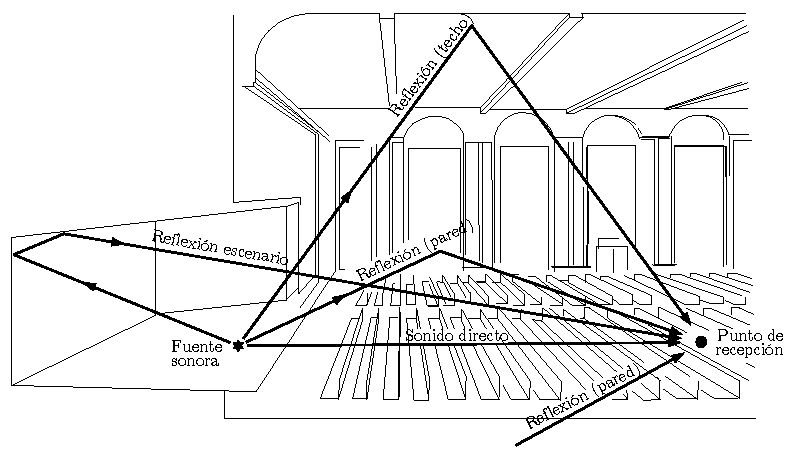
\includegraphics[width=0.7\textwidth]{archivos/geometrica.pdf}
    \caption{Ejemplo de llegada del sonido directo y de las primeras reflexiones a un receptor. Figura extraída y modificada de \cite{Carrión1998}, pág. 51.}
\end{figure}
\FloatBarrier

\subsection{Modos propios}
\label{modospropios}

Las ondas acústicas al reflejarse producen interferencias entre las ondas incidentes y las ondas reflejadas, estas interferencias pueden ser destructivas, reduciendo el nivel de presión acústica o constructivas, aumentando el nivel. Esto es parte de la acústica ondulatoria.

Este efecto, que se produce en posiciones y frecuencias concretas dentro de un recinto, se denomina modos propios. Para facilitar su comprensión se muestra en la figura \ref{graf:ondas} una onda incidente, la onda reflejada y el resultado frente a la distancia. Esto demuestra que es posible tener niveles menores o mayores de lo esperado en algunas posiciones de un recinto.

\begin{figure}[ht]
    \centering
    {\scalefont{0.8}
    %%%%%%%%%%%%%%%%%%%%%%%%%%%%%%%%%%%%%%%%%%%%%%%%%%%%%%%%%%%%%%%%%%%%%%%%
% Escuela Politécnica Superior de la Universidad de Alicante
% Realizado por: Jose Manuel Requena Plens
% Contacto: info@jmrplens.com / Telegram:@jmrplens
%%%%%%%%%%%%%%%%%%%%%%%%%%%%%%%%%%%%%%%%%%%%%%%%%%%%%%%%%%%%%%%%%%%%%%%%

\begin{tikzpicture}

\begin{axis}[%
width=0.5\textwidth,
height=0.15\textwidth,
at={(0\textwidth,0\textwidth)},
scale only axis,
xmin=0,
xmax=8,
xlabel style={font=\color{white!15!black}},
xlabel={Distancia (m)},
ymin=49.5,
ymax=50.5,
ylabel style={font=\color{white!15!black}},
ylabel={Nivel (dB)},
axis background/.style={fill=white},
 axis y line=left,
  axis x line=bottom,
  legend style={at={(0.5,1.05)}, anchor=south, legend cell align=left, align=left, draw=white!15!black,legend columns=-1}
]
\addplot [color=green, line width=1.0pt]
  table[row sep=crcr]{%
0	50\\
0.0638297872340416	50.0295520206661\\
0.106382978723403	50.0479425538604\\
0.148936170212764	50.0644217687238\\
0.170212765957444	50.07173560909\\
0.191489361702125	50.0783326909627\\
0.212765957446805	50.0841470984808\\
0.234042553191486	50.0891207360061\\
0.255319148936174	50.0932039085967\\
0.276595744680854	50.0963558185417\\
0.297872340425535	50.0985449729988\\
0.319148936170215	50.0997494986604\\
0.340425531914896	50.0999573603042\\
0.361702127659576	50.0991664810452\\
0.382978723404257	50.0973847630878\\
0.404255319148938	50.0946300087687\\
0.425531914893618	50.0909297426826\\
0.446808510638299	50.0863209366649\\
0.468085106382979	50.080849640382\\
0.48936170212766	50.0745705212177\\
0.51063829787234	50.0675463180551\\
0.553191489361701	50.0515501371821\\
0.595744680851062	50.0334988150156\\
0.659574468085104	50.0041580662433\\
0.723404255319146	49.9744458897973\\
0.765957446808514	49.9557479556705\\
0.808510638297875	49.9388142109057\\
0.829787234042556	49.9312233840816\\
0.851063829787236	49.9243197504692\\
0.872340425531917	49.9181722888936\\
0.893617021276597	49.9128424227586\\
0.914893617021278	49.9083834063251\\
0.936170212765958	49.904839792611\\
0.957446808510639	49.9022469882335\\
0.978723404255319	49.9006308996367\\
1	49.9000076742436\\
1.02127659574468	49.9003835391164\\
1.04255319148936	49.9017547387376\\
1.06382978723404	49.9041075725337\\
1.08510638297872	49.9074185317672\\
1.1063829787234	49.911654534428\\
1.12765957446808	49.9167732557776\\
1.14893617021276	49.9227235512444\\
1.17021276595744	49.929445967443\\
1.19148936170212	49.9368733362128\\
1.23404255319149	49.9535397820586\\
1.27659574468085	49.9720584501801\\
1.3404255319149	50.0016813900484\\
1.40425531914894	50.0311541363513\\
1.4468085106383	50.0494113351139\\
1.48936170212766	50.0656986598719\\
1.51063829787234	50.0728969040126\\
1.53191489361702	50.0793667863849\\
1.5531914893617	50.0850436620629\\
1.57446808510638	50.0898708095812\\
1.59574468085106	50.0937999976775\\
1.61702127659574	50.0967919672031\\
1.63829787234042	50.0988168233877\\
1.6595744680851	50.0998543345375\\
1.68085106382978	50.099894134184\\
1.70212765957447	50.0989358246623\\
1.72340425531915	50.0969889810845\\
1.74468085106383	50.094073055668\\
1.76595744680851	50.0902171833756\\
1.78723404255319	50.0854598908088\\
1.80851063829788	50.0798487112624\\
1.82978723404256	50.0734397097874\\
1.85106382978724	50.0662969230082\\
1.8936170212766	50.0501020856458\\
1.93617021276596	50.0319098362349\\
2	50.0024775425453\\
2.06382978723404	49.9728239373589\\
2.1063829787234	49.9542464106225\\
2.14893617021276	49.9374929351107\\
2.17021276595744	49.9300125312406\\
2.19148936170212	49.9232314190236\\
2.21276595744681	49.9172173530914\\
2.23404255319149	49.9120304240028\\
2.25531914893617	49.9077224578387\\
2.27659574468085	49.904336498373\\
2.29787234042553	49.9019063769934\\
2.31914893617022	49.9004563746694\\
2.3404255319149	49.9000009793449\\
2.36170212765958	49.9005447411796\\
2.38297872340426	49.9020822270849\\
2.40425531914894	49.9045980750098\\
2.42553191489362	49.9080671474335\\
2.4468085106383	49.9124547825312\\
2.46808510638298	49.9177171405031\\
2.48936170212766	49.9238016416081\\
2.51063829787234	49.9306474915223\\
2.53191489361702	49.9381862887763\\
2.57446808510638	49.9550352535465\\
2.61702127659574	49.9736768208634\\
2.70212765957447	50.013323204142\\
2.74468085106383	50.0327474439138\\
2.78723404255319	50.0508661464372\\
2.82978723404256	50.0669569762197\\
2.85106382978724	50.0740375889952\\
2.87234042553192	50.0803784426552\\
2.8936170212766	50.0859161814857\\
2.91489361702128	50.0905954742308\\
2.93617021276596	50.0943695669444\\
2.95744680851064	50.0972007501395\\
2.97872340425532	50.0990607355695\\
3	50.0999309388748\\
3.02127659574468	50.0998026652716\\
3.04255319148936	50.0986771964275\\
3.06382978723404	50.0965657776549\\
3.08510638297872	50.0934895055525\\
3.1063829787234	50.089479117214\\
3.12765957446808	50.0845746831143\\
3.14893617021276	50.0788252067375\\
3.17021276595744	50.0722881349512\\
3.19148936170212	50.0650287840157\\
3.23404255319149	50.0486398688854\\
3.27659574468085	50.0303118356746\\
3.3404255319149	50.0007963183786\\
3.40425531914894	49.9712096683335\\
3.4468085106383	49.9527578013601\\
3.48936170212766	49.9361893317652\\
3.51063829787234	49.9288214657631\\
3.53191489361702	49.9221647921466\\
3.5531914893617	49.916285822198\\
3.57446808510638	49.9112432966418\\
3.59574468085106	49.9070875987266\\
3.61702127659574	49.903860250812\\
3.63829787234042	49.9015934994918\\
3.6595744680851	49.9003099933958\\
3.68085106382978	49.9000225568927\\
3.70212765957447	49.9007340619529\\
3.72340425531915	49.9024373994532\\
3.74468085106383	49.9051155502082\\
3.76595744680851	49.9087417550209\\
3.78723404255319	49.9132797820514\\
3.80851063829788	49.9186842888339\\
3.82978723404256	49.9249012753228\\
3.85106382978724	49.9318686234445\\
3.8936170212766	49.9477691410373\\
3.93617021276596	49.965751938153\\
3.97872340425532	49.9851000974186\\
4.08510638297872	50.034331492882\\
4.12765957446808	50.0523065765158\\
4.17021276595744	50.0681963620068\\
4.19148936170212	50.0751573415352\\
4.21276595744681	50.0813673737507\\
4.23404255319149	50.0867644100642\\
4.25531914893617	50.0912945250728\\
4.27659574468085	50.0949124553648\\
4.29787234042553	50.0975820517767\\
4.31914893617022	50.0992766405836\\
4.3404255319149	50.0999792900143\\
4.36170212765958	50.0996829794279\\
4.38297872340426	50.0983906694619\\
4.40425531914894	50.0961152724502\\
4.42553191489362	50.0928795234077\\
4.4468085106383	50.0887157528692\\
4.46808510638298	50.0836655638536\\
4.48936170212766	50.0777794161801\\
4.51063829787234	50.0711161222906\\
4.53191489361702	50.063742259615\\
4.57446808510638	50.0471639003094\\
4.61702127659574	50.0287052651328\\
4.68085106382978	49.999114869071\\
4.74468085106383	49.9696035391189\\
4.78723404255319	49.951282548754\\
4.82978723404256	49.9349037694334\\
4.85106382978724	49.9276505243956\\
4.87234042553192	49.9211201714025\\
4.8936170212766	49.9153779595825\\
4.91489361702128	49.910481263218\\
4.93617021276596	49.9064790084805\\
4.95744680851064	49.9034111845764\\
4.97872340425532	49.9013084441879\\
5	49.9001917972021\\
5.02127659574468	49.9000724007863\\
5.04255319148936	49.9009514479103\\
5.06382978723404	49.9028201554256\\
5.08510638297872	49.9056598518245\\
5.1063829787234	49.9094421637993\\
5.12765957446808	49.914129299739\\
5.14893617021276	49.9196744273306\\
5.17021276595744	49.9260221414922\\
5.19148936170212	49.9331090179622\\
5.23404255319149	49.9492103409609\\
5.27659574468085	49.9673364873895\\
5.3404255319149	49.9967264620669\\
5.40425531914894	50.0264088521384\\
5.4468085106383	50.0450440594275\\
5.48936170212766	50.061883502212\\
5.51063829787234	50.0694164668252\\
5.53191489361702	50.076255845048\\
5.5531914893617	50.0823333000738\\
5.57446808510638	50.0875881079811\\
5.59574468085106	50.0919677644662\\
5.61702127659574	50.0954285094493\\
5.63829787234042	50.0979357643104\\
5.6595744680851	50.0994644773878\\
5.68085106382978	50.0999993742857\\
5.70212765957447	50.0995351104912\\
5.72340425531915	50.0980763247745\\
5.74468085106383	50.0956375928404\\
5.76595744680851	50.0922432816923\\
5.78723404255319	50.0879273061651\\
5.80851063829788	50.0827327900595\\
5.82978723404256	50.0767116352635\\
5.85106382978724	50.0699240031655\\
5.87234042553192	50.0624377135416\\
5.91489361702128	50.0456745972144\\
5.95744680851064	50.0270905788308\\
6.02127659574468	49.9974336700139\\
6.08510638297872	49.9680060038116\\
6.12765957446808	49.9498210698979\\
6.17021276595744	49.9336366115787\\
6.19148936170212	49.9265000381951\\
6.21276595744681	49.920097852134\\
6.23404255319149	49.9144940219223\\
6.25531914893617	49.909744539179\\
6.27659574468085	49.9058968591657\\
6.29787234042553	49.9029894266293\\
6.31914893617022	49.9010512916745\\
6.3404255319149	49.9001018195053\\
6.36170212765958	49.9001504969336\\
6.38297872340426	49.9011968375907\\
6.40425531914894	49.9032303867866\\
6.42553191489362	49.90623082597\\
6.4468085106383	49.9101681757443\\
6.46808510638298	49.9150030954121\\
6.48936170212766	49.9206872760543\\
6.51063829787234	49.9271639232168\\
6.53191489361702	49.9343683243822\\
6.57446808510638	49.9506659005043\\
6.61702127659574	49.9689302714906\\
6.68085106382978	49.99840741374\\
6.74468085106383	50.0280268169769\\
6.78723404255319	50.0465388476355\\
6.82978723404256	50.0631955213007\\
6.85106382978724	50.070616945718\\
6.87234042553192	50.0773327889566\\
6.8936170212766	50.0832759485308\\
6.91489361702128	50.0883870423546\\
6.93617021276596	50.0926150020681\\
6.95744680851064	50.0959175832953\\
6.97872340425532	50.0982617877364\\
7	50.0996241928755\\
7.02127659574468	50.0999911860107\\
7.04255319148936	50.099359100268\\
7.06382978723404	50.0977342512392\\
7.08510638297872	50.0951328738787\\
7.1063829787234	50.0915809602891\\
7.12765957446808	50.0871140000169\\
7.14893617021276	50.0817766254526\\
7.17021276595744	50.0756221658786\\
7.19148936170213	50.0687121146205\\
7.21276595744681	50.0611155146263\\
7.25531914893617	50.0441723806669\\
7.29787234042553	50.0254682332844\\
7.4468085106383	49.9571817330504\\
7.48936170212766	49.9400816550786\\
7.51063829787234	49.9323882164612\\
7.53191489361702	49.9253703324355\\
7.5531914893617	49.9190981233788\\
7.57446808510638	49.9136342591307\\
7.59574468085106	49.9090333328166\\
7.61702127659574	49.9053413153715\\
7.63829787234042	49.9025950962132\\
7.6595744680851	49.9008221146557\\
7.68085106382978	49.9000400857447\\
7.70212765957447	49.9002568232546\\
};
\addlegendentry{Onda incidente}

\addplot [color=blue, line width=1.0pt]
  table[row sep=crcr]{%
0	50.05\\
0.0425531914893611	50.0662085976342\\
0.0638297872340416	50.0733596250863\\
0.0851063829787222	50.079777667414\\
0.106382978723403	50.0853985976599\\
0.127659574468083	50.0901662533471\\
0.148936170212764	50.0940329976357\\
0.170212765957444	50.0969601952952\\
0.191489361702125	50.0989185987341\\
0.212765957446805	50.0998886402325\\
0.234042553191486	50.0998606274566\\
0.255319148936174	50.0988348403006\\
0.276595744680854	50.0968215280908\\
0.297872340425535	50.0938408071773\\
0.319148936170215	50.0899224599381\\
0.340425531914896	50.0851056372036\\
0.361702127659576	50.0794384670743\\
0.382978723404257	50.0729775740409\\
0.404255319148938	50.0657875132109\\
0.446808510638299	50.0495138188003\\
0.48936170212766	50.031266164684\\
0.553191489361701	50.0017992906999\\
0.617021276595743	49.9721716914363\\
0.659574468085104	49.9536442334837\\
0.702127659574465	49.936964833658\\
0.723404255319146	49.9295295817644\\
0.744680851063826	49.9227984469954\\
0.765957446808514	49.9168386846246\\
0.787234042553195	49.9117098426275\\
0.808510638297875	49.907463166698\\
0.829787234042556	49.9041410882183\\
0.851063829787236	49.9017768002984\\
0.872340425531917	49.9003939261216\\
0.893617021276597	49.9000062829096\\
0.914893617021278	49.9006177438653\\
0.936170212765958	49.9022221994729\\
0.957446808510639	49.9048036185422\\
0.978723404255319	49.9083362083874\\
1	49.9127846725383\\
1.02127659574468	49.9181045634117\\
1.04255319148936	49.9242427264164\\
1.06382978723404	49.9311378310568\\
1.08510638297872	49.9387209837264\\
1.12765957446808	49.9556422420381\\
1.17021276595744	49.9743319041807\\
1.31914893617022	50.0426313514886\\
1.36170212765958	50.0597527031571\\
1.38297872340426	50.067459318741\\
1.40425531914894	50.0744919031112\\
1.42553191489362	50.0807801890092\\
1.4468085106383	50.086261345961\\
1.46808510638298	50.0908806080582\\
1.48936170212766	50.0945918211608\\
1.51063829787234	50.0973579040543\\
1.53191489361702	50.0991512189527\\
1.5531914893617	50.0999538476463\\
1.57446808510638	50.0997577705347\\
1.59574468085106	50.0985649467554\\
1.61702127659574	50.0963872946093\\
1.63829787234042	50.0932465724769\\
1.6595744680851	50.0891741614156\\
1.68085106382978	50.0842107516104\\
1.70212765957447	50.0784059358115\\
1.72340425531915	50.0718177138196\\
1.74468085106383	50.0645119129709\\
1.78723404255319	50.0480460037393\\
1.82978723404256	50.0296646519565\\
1.8936170212766	50.0001179184898\\
1.95744680851064	49.9705606517156\\
2	49.9521609626815\\
2.04255319148936	49.9356684651004\\
2.06382978723404	49.9283465953864\\
2.08510638297872	49.9217406628059\\
2.1063829787234	49.9159166716535\\
2.12765957446808	49.9109328133237\\
2.14893617021276	49.9068388848814\\
2.17021276595744	49.9036757915065\\
2.19148936170212	49.9014751377822\\
2.21276595744681	49.9002589119133\\
2.23404255319149	49.9000392660265\\
2.25531914893617	49.9008183947509\\
2.27659574468085	49.90258851329\\
2.29787234042553	49.9053319352042\\
2.31914893617022	49.9090212491288\\
2.3404255319149	49.9136195926585\\
2.36170212765958	49.9190810206649\\
2.38297872340426	49.9253509643644\\
2.40425531914894	49.9323667765524\\
2.4468085106383	49.9483488556298\\
2.48936170212766	49.9663901028386\\
2.5531914893617	49.9957241201395\\
2.61702127659574	50.0254400890537\\
2.6595744680851	50.0441462691656\\
2.70212765957447	50.0610924768375\\
2.72340425531915	50.0686909672612\\
2.74468085106383	50.0756031202463\\
2.76595744680851	50.081759871845\\
2.78723404255319	50.0870997058304\\
2.80851063829788	50.0915692683465\\
2.82978723404256	50.095123901002\\
2.85106382978724	50.0977280870825\\
2.87234042553192	50.0993558064215\\
2.8936170212766	50.0999907953854\\
2.91489361702128	50.0996267093743\\
2.93617021276596	50.0982671862154\\
2.95744680851064	50.0959258098147\\
2.97872340425532	50.0926259744311\\
3	50.0884006509291\\
3.02127659574468	50.0832920573444\\
3.04255319148936	50.0773512370554\\
3.06382978723404	50.0706375487747\\
3.08510638297872	50.0632180734562\\
3.12765957446808	50.0465646047645\\
3.17021276595744	50.028054752224\\
3.23404255319149	49.9984365129409\\
3.29787234042553	49.9689579353004\\
3.3404255319149	49.9506912172779\\
3.38297872340426	49.9343902848196\\
3.40425531914894	49.9271838673773\\
3.42553191489362	49.9207050046622\\
3.4468085106383	49.9150184313292\\
3.46808510638298	49.9101809657391\\
3.48936170212766	49.9062409422491\\
3.51063829787234	49.9032377282716\\
3.53191489361702	49.9012013309278\\
3.5531914893617	49.9001520972269\\
3.57446808510638	49.9001005107651\\
3.59574468085106	49.9010470869774\\
3.61702127659574	49.9029823679872\\
3.63829787234042	49.9058870171062\\
3.6595744680851	49.9097320120408\\
3.68085106382978	49.9144789348723\\
3.70212765957447	49.9200803559172\\
3.72340425531915	49.9264803076278\\
3.74468085106383	49.9336148438021\\
3.78723404255319	49.9497958983742\\
3.82978723404256	49.96797843205\\
3.8936170212766	49.9974045768834\\
3.95744680851064	50.027062563134\\
4	50.04564870549\\
4.04255319148936	50.062414978011\\
4.06382978723404	50.0699031949744\\
4.08510638297872	50.0766929623205\\
4.1063829787234	50.0827164389384\\
4.12765957446808	50.0879134402409\\
4.14893617021276	50.0922320395088\\
4.17021276595744	50.0956290867259\\
4.19148936170212	50.0980706397191\\
4.21276595744681	50.0995323032981\\
4.23404255319149	50.0999994730035\\
4.25531914893617	50.0994674810301\\
4.27659574468085	50.0979416428659\\
4.29787234042553	50.0954372041813\\
4.31914893617022	50.0919791884999\\
4.3404255319149	50.0876021471713\\
4.36170212765958	50.0823498141455\\
4.38297872340426	50.0762746689981\\
4.40425531914894	50.0694374125711\\
4.42553191489362	50.0619063604706\\
4.46808510638298	50.045070040708\\
4.51063829787234	50.026436920649\\
4.59574468085106	49.9867936723521\\
4.63829787234042	49.9673639953223\\
4.68085106382978	49.94923541281\\
4.72340425531915	49.9331306541922\\
4.74468085106383	49.9260417264718\\
4.76595744680851	49.9196917653732\\
4.78723404255319	49.9141442176086\\
4.80851063829788	49.9094545124415\\
4.82978723404256	49.9056695078558\\
4.85106382978724	49.902827022366\\
4.87234042553192	49.9009554571476\\
4.8936170212766	49.9000735122617\\
4.91489361702128	49.9001899998099\\
4.93617021276596	49.9013037558872\\
4.95744680851064	49.9034036522111\\
4.97872340425532	49.9064687073115\\
5	49.9104682961712\\
5.02127659574468	49.9153624562203\\
5.04255319148936	49.9211022866293\\
5.06382978723404	49.9276304369103\\
5.08510638297872	49.9348816799434\\
5.12765957446808	49.9512571351854\\
5.17021276595744	49.9695758146306\\
5.23404255319149	49.9990857674241\\
5.29787234042553	50.0286773858907\\
5.3404255319149	50.0471382356822\\
5.38297872340426	50.0637198327704\\
5.40425531914894	50.0710956591506\\
5.42553191489362	50.0777611212056\\
5.4468085106383	50.083649619842\\
5.46808510638298	50.0887023191277\\
5.48936170212766	50.0928687341619\\
5.51063829787234	50.0961072355026\\
5.53191489361702	50.098385465115\\
5.5531914893617	50.0996806596819\\
5.57446808510638	50.0999798780473\\
5.59574468085106	50.0992801305202\\
5.61702127659574	50.0975884087466\\
5.63829787234042	50.0949216158512\\
5.6595744680851	50.0913063975472\\
5.68085106382978	50.0867788759007\\
5.70212765957447	50.0813842884115\\
5.72340425531915	50.0751765360146\\
5.74468085106383	50.0682176445199\\
5.78723404255319	50.0523313784145\\
5.82978723404256	50.034358825393\\
5.87234042553192	50.0150164944285\\
5.97872340425532	49.9657792824314\\
6.02127659574468	49.9477939608735\\
6.06382978723404	49.9318899293498\\
6.08510638297872	49.9249204955844\\
6.1063829787234	49.9187012314092\\
6.12765957446808	49.9132942776559\\
6.14893617021276	49.9087536588192\\
6.17021276595744	49.9051247432615\\
6.19148936170212	49.9024437899076\\
6.21276595744681	49.9007375859571\\
6.23404255319149	49.9000231792359\\
6.25531914893617	49.9003077078599\\
6.27659574468085	49.901588328913\\
6.29787234042553	49.9038522468531\\
6.31914893617022	49.9070768413604\\
6.3404255319149	49.9112298933525\\
6.36170212765958	49.9162699069068\\
6.38297872340426	49.9221465238737\\
6.40425531914894	49.9288010270391\\
6.42553191489362	49.9361669268072\\
6.46808510638298	49.9527321529319\\
6.51063829787234	49.971181798957\\
6.57446808510638	50.0007672164432\\
6.63829787234042	50.0302841007695\\
6.68085106382978	50.0486144386115\\
6.72340425531915	50.0650066721979\\
6.74468085106383	50.0722680226478\\
6.76595744680851	50.0788072949041\\
6.78723404255319	50.0845591507199\\
6.80851063829788	50.0894661194533\\
6.82978723404256	50.0934791722947\\
6.85106382978724	50.0965582121466\\
6.87234042553192	50.0986724742606\\
6.8936170212766	50.0998008336286\\
6.91489361702128	50.0999320160568\\
6.93617021276596	50.0990647108136\\
6.95744680851064	50.0972075837265\\
6.97872340425532	50.0943791905953\\
7	50.0906077917893\\
7.02127659574468	50.0859310698787\\
7.04255319148936	50.0803957531229\\
7.06382978723404	50.0740571485772\\
7.08510638297872	50.0669785894829\\
7.12765957446808	50.0508912008434\\
7.17021276595744	50.0327749406228\\
7.23404255319149	50.003391390949\\
7.29787234042553	49.9737048984222\\
7.3404255319149	49.9550612502714\\
7.38297872340426	49.9382091682599\\
7.40425531914894	49.9306684610792\\
7.42553191489362	49.9238204917176\\
7.4468085106383	49.917733682821\\
7.46808510638298	49.9124688517721\\
7.48936170212766	49.9080786030224\\
7.51063829787234	49.904606802486\\
7.53191489361702	49.9020881392465\\
7.5531914893617	49.9005477789542\\
7.57446808510638	49.9000011123801\\
7.59574468085106	49.9004536016358\\
7.61702127659574	49.9019007255983\\
7.63829787234042	49.9043280250834\\
7.6595744680851	49.9077112473168\\
7.68085106382978	49.9120165882605\\
7.70212765957447	49.9172010303708\\
};
\addlegendentry{Onda reflejada}

\addplot [color=red, line width=1.5pt]
  table[row sep=crcr]{%
0	50.05\\
0.0425531914893611	50.0860755307137\\
0.0638297872340416	50.1029116457524\\
0.0851063829787222	50.1187195016449\\
0.106382978723403	50.1333411515204\\
0.127659574468083	50.1466305006866\\
0.148936170212764	50.1584547663595\\
0.170212765957444	50.1686958043852\\
0.191489361702125	50.1772512896968\\
0.212765957446805	50.1840357387133\\
0.234042553191486	50.1889813634627\\
0.255319148936174	50.1920387488973\\
0.276595744680854	50.1931773466325\\
0.297872340425535	50.1923857801761\\
0.319148936170215	50.1896719585985\\
0.340425531914896	50.1850629975077\\
0.361702127659576	50.1786049481196\\
0.382978723404257	50.1703623371287\\
0.404255319148938	50.1604175219796\\
0.425531914893618	50.1488698679779\\
0.446808510638299	50.1358347554652\\
0.468085106382979	50.1214424269768\\
0.48936170212766	50.1058366859016\\
0.51063829787234	50.0891734596459\\
0.553191489361701	50.053349427882\\
0.595744680851062	50.0153985227823\\
0.659574468085104	49.957802299727\\
0.702127659574465	49.9211902642437\\
0.723404255319146	49.9039754715617\\
0.744680851063826	49.8877201242264\\
0.765957446808514	49.8725866402951\\
0.787234042553195	49.8587262285366\\
0.808510638297875	49.8462773776038\\
0.829787234042556	49.8353644722999\\
0.851063829787236	49.8260965507676\\
0.872340425531917	49.8185662150152\\
0.893617021276597	49.8128487056683\\
0.914893617021278	49.8090011501904\\
0.936170212765958	49.8070619920839\\
0.957446808510639	49.8070506067757\\
0.978723404255319	49.808967108024\\
1	49.8127923467819\\
1.02127659574468	49.8184881025281\\
1.04255319148936	49.825997465154\\
1.06382978723404	49.8352454035905\\
1.08510638297872	49.8461395154936\\
1.1063829787234	49.8585709504985\\
1.12765957446808	49.8724154978157\\
1.14893617021276	49.8875348273049\\
1.17021276595744	49.9037778716237\\
1.19148936170212	49.9209823356424\\
1.23404255319149	49.9575800289031\\
1.36170212765958	50.0714076236421\\
1.38297872340426	50.0889713175498\\
1.40425531914894	50.1056460394625\\
1.42553191489362	50.1212651810708\\
1.4468085106383	50.1356726810749\\
1.46808510638298	50.148724584497\\
1.48936170212766	50.1602904810327\\
1.51063829787234	50.1702548080669\\
1.53191489361702	50.1785180053376\\
1.5531914893617	50.1849975097092\\
1.57446808510638	50.1896285801158\\
1.59574468085106	50.1923649444328\\
1.61702127659574	50.1931792618125\\
1.63829787234042	50.1920633958646\\
1.6595744680851	50.189028495953\\
1.68085106382978	50.1841048857944\\
1.70212765957447	50.1773417604739\\
1.72340425531915	50.1688066949041\\
1.74468085106383	50.1585849686389\\
1.76595744680851	50.1467787137883\\
1.78723404255319	50.1335058945481\\
1.80851063829788	50.1188991285408\\
1.82978723404256	50.1031043617439\\
1.85106382978724	50.0862794102462\\
1.8936170212766	50.0502200041356\\
1.95744680851064	49.9928496431256\\
2	49.9546385052268\\
2.04255319148936	49.9182357869781\\
2.06382978723404	49.9011705327453\\
2.08510638297872	49.8850927498807\\
2.1063829787234	49.8701630822759\\
2.12765957446808	49.8565307022347\\
2.14893617021276	49.8443318199921\\
2.17021276595744	49.8336883227471\\
2.19148936170212	49.8247065568059\\
2.21276595744681	49.8174762650047\\
2.23404255319149	49.8120696900293\\
2.25531914893617	49.8085408525897\\
2.27659574468085	49.8069250116629\\
2.29787234042553	49.8072383121976\\
2.31914893617022	49.8094776237982\\
2.3404255319149	49.8136205720035\\
2.36170212765958	49.8196257618445\\
2.38297872340426	49.8274331914493\\
2.40425531914894	49.8369648515622\\
2.42553191489362	49.848125504986\\
2.4468085106383	49.860803638161\\
2.46808510638298	49.8748725753712\\
2.48936170212766	49.8901917444467\\
2.51063829787234	49.906608081314\\
2.53191489361702	49.9239575593614\\
2.57446808510638	49.9607549464186\\
2.68085106382978	50.0562458753018\\
2.72340425531915	50.0918419497714\\
2.74468085106383	50.1083505641601\\
2.76595744680851	50.1237765755276\\
2.78723404255319	50.1379658522676\\
2.80851063829788	50.1507766198172\\
2.82978723404256	50.1620808772217\\
2.85106382978724	50.1717656760778\\
2.87234042553192	50.1797342490767\\
2.8936170212766	50.185906976871\\
2.91489361702128	50.1902221836052\\
2.93617021276596	50.1926367531599\\
2.95744680851064	50.1931265599542\\
2.97872340425532	50.1916867100006\\
3	50.1883315898039\\
3.02127659574468	50.1830947226161\\
3.04255319148936	50.1760284334829\\
3.06382978723404	50.1672033264296\\
3.08510638297872	50.1567075790087\\
3.1063829787234	50.144646061259\\
3.12765957446808	50.1311392878788\\
3.14893617021276	50.1163222140831\\
3.17021276595744	50.1003428871752\\
3.19148936170212	50.0833609673076\\
3.23404255319149	50.0470763818263\\
3.29787234042553	49.9896046834942\\
3.3404255319149	49.9514875356565\\
3.38297872340426	49.9153044266822\\
3.40425531914894	49.8983935357108\\
3.42553191489362	49.8824978629438\\
3.4468085106383	49.8677762326893\\
3.46808510638298	49.8543757386104\\
3.48936170212766	49.8424302740143\\
3.51063829787234	49.8320591940346\\
3.53191489361702	49.8233661230743\\
3.5531914893617	49.8164379194249\\
3.57446808510638	49.811343807407\\
3.59574468085106	49.808134685704\\
3.61702127659574	49.8068426187992\\
3.63829787234042	49.8074805165981\\
3.6595744680851	49.8100420054366\\
3.68085106382978	49.814501491765\\
3.70212765957447	49.8208144178701\\
3.72340425531915	49.8289177070809\\
3.74468085106383	49.8387303940103\\
3.76595744680851	49.8501544335341\\
3.78723404255319	49.8630756804257\\
3.80851063829788	49.8773650298573\\
3.82978723404256	49.8928797073728\\
3.85106382978724	49.909464695443\\
3.8936170212766	49.9451737179207\\
3.93617021276596	49.9830684912506\\
4	50.0406951414022\\
4.04255319148936	50.0774026989773\\
4.06382978723404	50.0946866157727\\
4.08510638297872	50.1110244552025\\
4.1063829787234	50.1262529749757\\
4.12765957446808	50.1402200167567\\
4.14893617021276	50.1527860264808\\
4.17021276595744	50.1638254487327\\
4.19148936170212	50.1732279812543\\
4.21276595744681	50.1808996770488\\
4.23404255319149	50.1867638830677\\
4.25531914893617	50.1907620061029\\
4.27659574468085	50.1928540982306\\
4.29787234042553	50.193019255958\\
4.31914893617022	50.1912558290835\\
4.3404255319149	50.1875814371855\\
4.36170212765958	50.1820327935734\\
4.38297872340426	50.17466533846\\
4.40425531914894	50.1655526850213\\
4.42553191489362	50.1547858838783\\
4.4468085106383	50.1424725133491\\
4.46808510638298	50.1287356045616\\
4.48936170212766	50.1137124121676\\
4.51063829787234	50.0975530429396\\
4.53191489361702	50.0804189559533\\
4.57446808510638	50.0439194497419\\
4.70212765957447	49.9300240587693\\
4.72340425531915	49.9123970121315\\
4.74468085106383	49.8956452655907\\
4.76595744680851	49.8799361970611\\
4.78723404255319	49.8654267663626\\
4.80851063829788	49.8522619469306\\
4.82978723404256	49.8405732772892\\
4.85106382978724	49.8304775467616\\
4.87234042553192	49.8220756285501\\
4.8936170212766	49.8154514718442\\
4.91489361702128	49.8106712630279\\
4.93617021276596	49.8077827643678\\
4.95744680851064	49.8068148367875\\
4.97872340425532	49.8077771514995\\
5	49.8106600933733\\
5.02127659574468	49.8154348570066\\
5.04255319148936	49.8220537345396\\
5.06382978723404	49.8304505923359\\
5.08510638297872	49.840541531768\\
5.1063829787234	49.8522257275047\\
5.12765957446808	49.8653864349244\\
5.14893617021276	49.8798921565891\\
5.17021276595744	49.8955979561228\\
5.19148936170212	49.9123469063682\\
5.23404255319149	49.948296108385\\
5.27659574468085	49.9863065813994\\
5.3404255319149	50.0438646977492\\
5.38297872340426	50.0803678331241\\
5.40425531914894	50.097504511289\\
5.42553191489362	50.1136669566078\\
5.4468085106383	50.1286936792695\\
5.46808510638298	50.1424345372284\\
5.48936170212766	50.1547522363739\\
5.51063829787234	50.1655237023278\\
5.53191489361702	50.174641310163\\
5.5531914893617	50.1820139597557\\
5.57446808510638	50.1875679860284\\
5.59574468085106	50.1912478949864\\
5.61702127659574	50.1930169181958\\
5.63829787234042	50.1928573801616\\
5.6595744680851	50.1907708749349\\
5.68085106382978	50.1867782501864\\
5.70212765957447	50.1809193989027\\
5.72340425531915	50.1732528607892\\
5.74468085106383	50.1638552373604\\
5.76595744680851	50.1528204265632\\
5.78723404255319	50.1402586845796\\
5.80851063829788	50.126295524183\\
5.82978723404256	50.1110704606565\\
5.85106382978724	50.0947356178022\\
5.87234042553192	50.0774542079702\\
5.91489361702128	50.0407501004329\\
6.04255319148936	49.9270063338173\\
6.06382978723404	49.9095143653311\\
6.08510638297872	49.892926499396\\
6.1063829787234	49.8774084764851\\
6.12765957446808	49.8631153475538\\
6.14893617021276	49.8501899248217\\
6.17021276595744	49.8387613548402\\
6.19148936170212	49.8289438281027\\
6.21276595744681	49.8208354380911\\
6.23404255319149	49.8145172011582\\
6.25531914893617	49.8100522470389\\
6.27659574468085	49.8074851880788\\
6.29787234042553	49.8068416734824\\
6.31914893617022	49.808128133035\\
6.3404255319149	49.8113317128578\\
6.36170212765958	49.8164204038404\\
6.38297872340426	49.8233433614644\\
6.40425531914894	49.8320314138258\\
6.42553191489362	49.8423977527771\\
6.4468085106383	49.8543388012864\\
6.46808510638298	49.867735248344\\
6.48936170212766	49.8824532410792\\
6.51063829787234	49.8983457221738\\
6.53191489361702	49.91525389921\\
6.57446808510638	49.9514331169475\\
6.63829787234042	50.0088588467399\\
6.68085106382978	50.0470218523515\\
6.72340425531915	50.0833102450959\\
6.74468085106383	50.1002948396247\\
6.76595744680851	50.116277321269\\
6.78723404255319	50.1310979983554\\
6.80851063829788	50.1446087875775\\
6.82978723404256	50.1566746935954\\
6.85106382978724	50.1671751578646\\
6.87234042553192	50.1760052632172\\
6.8936170212766	50.1830767821594\\
6.91489361702128	50.1883190584114\\
6.93617021276596	50.1916797128817\\
6.95744680851064	50.1931251670218\\
6.97872340425532	50.1926409783317\\
7	50.1902319846648\\
7.02127659574468	50.1859222558894\\
7.04255319148936	50.1797548533909\\
7.06382978723404	50.1717913998164\\
7.08510638297872	50.1621114633616\\
7.1063829787234	50.1508117627518\\
7.12765957446808	50.1380052008603\\
7.14893617021276	50.1238197366203\\
7.17021276595744	50.1083971065014\\
7.19148936170213	50.0918914083256\\
7.21276595744681	50.0744675615731\\
7.25531914893617	50.0375692299608\\
7.36170212765958	49.9421204655342\\
7.38297872340426	49.9240092461625\\
7.40425531914894	49.9066573012839\\
7.42553191489362	49.8902380057958\\
7.4468085106383	49.8749154158714\\
7.46808510638298	49.8608426297641\\
7.48936170212766	49.8481602581009\\
7.51063829787234	49.8369950189473\\
7.53191489361702	49.827458471682\\
7.5531914893617	49.819645902333\\
7.57446808510638	49.8136353715108\\
7.59574468085106	49.8094869344525\\
7.61702127659574	49.8072420409698\\
7.63829787234042	49.8069231212965\\
7.6595744680851	49.8085333619725\\
7.68085106382978	49.8120566740052\\
7.70212765957447	49.8174578536254\\
};
\addlegendentry{Nivel resultante}
\draw[line width=1.5pt,  pattern=bricks, pattern color=brown] (axis cs:7.7,49) rectangle (axis cs:8,51);
\end{axis}
\end{tikzpicture}%
    }
    \caption{Ejemplo básico de interferencia de ondas (100 Hz) en dos dimensiones frente a la distancia.}
    \label{graf:ondas}
\end{figure}
\FloatBarrier

Los modos propios varían según las dimensiones del recinto, es por ello por lo que se denomina \textit{propio} pues cada recinto producirá unos modos.

Es posible calcular las frecuencias que van a producir un modo propio para un recinto rectangular con:

\begin{flalign}
	f = \frac{c}{2}\sqrt{ \left(\frac{n_x}{L_x}\right)^2 +\left(\frac{n_y}{L_y}\right)^2 +\left(\frac{n_z}{L_z}\right)^2 }
\end{flalign}

\begin{condiciones}[Donde:]
	n_x,n_y,n_z & \rightarrow & Son los índices para cada modo propio. 0,1,2,3,...\\
	L_x,L_y,L_z & \rightarrow & Son las dimensiones del recinto, largo, ancho y alto en metros.\\
	c & \rightarrow & Es la velocidad del sonido en el aire.
\end{condiciones}

Los modos propios en un recinto rectangular pueden ser:
\begin{description}
\itemsep0em
	\item[Axiales:] Son los modos producidos entre dos superficies (techo y suelo, pared izquierda y pared derecha, pared frontal y posterior). Las combinaciones de índices pueden ser: ($n_x$,$0$,$0$) ; ($0$,$n_y$,$0$) ; ($0$,$0$,$n_z$).
	\item[Tangenciales:] Son los modos producidos entre cuatro superficies, es decir, entre aristas enfrentadas (suelo+pared izquierda y techo+pared derecha, ...). Las combinaciones de índices pueden ser: ($n_x$,$n_y$,$0$) ; ($n_x$,$0$,$n_z$) ; ($0$,$n_y$,$n_z$).
	\item[Oblicuos:] Son los modos producidos entre seis superficies, es decir, vértices enfrentados. Las combinaciones de índices pueden ser: ($n_x$,$n_y$,$n_z$).
\end{description}

La diferencia de nivel en distintas posiciones se va reduciendo cuando la densidad modal (número de modos en una frecuencia o banda de frecuencia) aumenta, llegando a ser imperceptible. El cálculo de la densidad modal desde 0 a una frecuencia determinado por \cite{Morse1968} se obtiene como:
\begin{flalign}
	Dn (f) = \frac{4\pi Vf^3}{3c^3} + \frac{\pi S f^2}{4c^2} + \frac{Lf}{8c}
\end{flalign}
\begin{condiciones}[Donde:]
	V & \rightarrow & Es el volumen del recinto en $m^3$.\\
	S & \rightarrow & Es la superficie del recinto en $m^2$.\\
	L & \rightarrow & Es el perímetro del recinto en $m$.\\
	f & \rightarrow & Es la frecuencia límite para el cálculo.
\end{condiciones}

Derivando esta ecuación como indica \cite{Mankovsky1971} se puede obtener la densidad modal para una frecuencia concreta:
\begin{flalign}
	Dn(f_i) = \frac{4\pi Vf_i^2}{3c^3} + \frac{\pi S f_i}{4c^2} + \frac{L}{8c}
\end{flalign}

Se puede obtener una aproximación de la densidad modal en una banda de octava o tercio de octava completa mediante:
\begin{flalign}
	Dn(f_i,\Delta f_i) = \left( \frac{4\pi Vf_i^2}{3c^3} + \frac{\pi S f_i}{4c^2} + \frac{L}{8c} \right) \Delta f_i \label{ecu:densmodal}
\end{flalign}
\begin{condiciones}[Donde:]
	f_i & \rightarrow & Es la frecuencia central de la banda.\\
	\Delta f_i & \rightarrow & Es el ancho de la banda.
\end{condiciones}

Es posible conocer a partir de que frecuencia la respuesta modal no será apreciable por una persona (debido al número de modos que contiene) y por tanto más allá de esa frecuencia no tiene importancia estudiar la respuesta modal. El cálculo, definido por \cite{schroeder1954}, tenía en cuenta a partir de qué frecuencia se producían mínimo 10 modos en todas las bandas y revisado en \cite{Schroeder1962} donde aclaró que era suficiente con 3 modos. Debido al estudio de Schroeder la ecuación recibió el nombre de \textit{frecuencia de Schroeder} también conocida como frecuencia límite o de cruce:
\begin{flalign}
	f_s = 2000 \sqrt{\frac{T}{V}}\label{ecu:schroeder}
\end{flalign}
\begin{condiciones}[Donde:]
	T & \rightarrow & Es el tiempo medio de reverberación (entre 500 Hz y 1 KHz) en segundos.\\
	V & \rightarrow & Es el volumen del recinto en $m^3$.
\end{condiciones}

\subsection{Coeficiente de absorción medio}
\label{coefmedioabs}
La absorción acústica es la disipación de la energía acústica al paso de ésta por un material. Los materiales absorbentes son diseñados para producir esta disipación a ciertas frecuencias sobre las que se desea actuar. Debido a que el propósito de este trabajo no es profundizar en el funcionamiento y diseño de estos materiales, si se tiene interés se recomienda la lectura de \cite{Cox2016}, donde se desarrollan todos los conceptos sobre los materiales para el acondicionamiento acústico de recintos.

El coeficiente de absorción de los materiales se suele ofrecer u obtener por bandas de frecuencia, pero en algunos cálculos es necesario un coeficiente global, en el documento DB-HR del Código Técnico de la Edificación (\textit{sección 3.2}) se indica que este coeficiente se obtiene realizando el promedio del coeficiente de absorción en las bandas de 500 Hz, 1000 Hz y 2000 Hz (ecuación \ref{ecu:coefmedio}). Estos coeficientes no tienen unidades y comprenden un valor entre 0 y 1, donde 0 es reflexión total y 1 es la absorción total.

\begin{flalign}
 	\alpha_{mid} =& \frac{\alpha_{500}+\alpha_{1000}+\alpha_{2000}}{3}\label{ecu:coefmedio}
 \end{flalign}

\subsection{Absorción acústica}

Para los cálculos acústicos, en ocasiones, se utiliza el valor de absorción total o equivalente del recinto; éste se calcula como la suma de las áreas de absorción por su coeficiente de absorción (medio o por bandas). Las unidades de absorción son los $m^2$.

\begin{flalign}
	A_T = \sum_{i=1}^n S_i \alpha_i
\end{flalign}
\begin{condiciones}[Donde:]
S_i & \rightarrow & Es la superficie del material $i$ en $m^2$.\\
\alpha_i & \rightarrow & Es el coeficiente de absorción del material $i$, no tiene unidades. El valor se encuentra entre $0$ y $1$.	
\end{condiciones}

\subsection{Constante del recinto}
 La constante del recinto es un valor que relaciona la absorción media de las superficies del recinto y el área. Se representa con las letras $Rc$ provenientes de \textit{room constant} y sus unidades son los $m^2$.
 
 \begin{flalign}
 	Rc =& \frac{A_T}{1-\overline{\alpha}}
 \end{flalign}
\begin{condiciones}[Donde:]
	\overline{\alpha} & = & $\nicefrac{A_T}{S}$, es el coeficiente medio de absorción, no confundir con coeficiente de absorción medio (\ref{coefmedioabs}).\\
	S & \rightarrow & Es el área total de todas las superficies.
\end{condiciones}

\subsection{Camino libre medio en acústica}

El camino libre medio (en inglés \textit{mean free path}) o MFP aplicado a la acústica geométrica, describe la distancia media que recorre el sonido entre una reflexión y otra.
\cite{jager1911theorie} propuso utilizar una modificación de la teoría cinética de los gases \cite[][cap. 10]{Bernoulli1738a}, obteniendo así el valor del camino libre medio para ondas acústicas como:

\begin{flalign}
	\text{MFP}=4\frac{V}{S}
\end{flalign}
\begin{condiciones}[Donde:]
	V & \rightarrow & Es el volumen del recinto en $m^3$.\\
	S & \rightarrow & Es la suma del área de todas las superficies del recinto en $m^2$.
\end{condiciones}

\citeauthor{jager1911theorie} demostró teóricamente que este valor para MFP es válido para cualquier factor de forma de recinto en el supuesto de que la distribución de energía acústica sea uniforme.
Años más tarde, \cite{Schuster1929} y \cite{Eyring1930} obtuvieron otros valores de MFP para recintos con factores de forma muy concretos:
\begin{flalign*}
	&&\text{Cubo } &\rightarrow \text{MFP}=2\sqrt{3}\frac{V}{S}&&\\
	&&\text{Cilindro (altura=diámetro)} &\rightarrow \text{MFP}=3\sqrt{2}\frac{V}{S}&&\\
	&&\text{Esfera }&\rightarrow \text{MFP}=\text{diámetro}=6\frac{V}{S}&&
\end{flalign*}

\begin{figure}[ht]
    \centering
    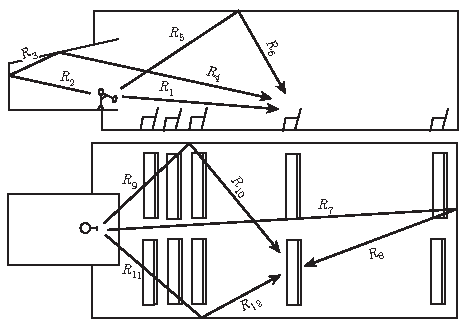
\includegraphics[width=0.8\textwidth]{archivos/mfp.pdf}
    \caption{Trazado de rayos para calcular el camino libre medio (promedio de $R_i$). Figura extraída y modificada de \cite{Self2009}, pág. 109.}
\end{figure}

Poco después, \cite{Knudsen1932} demostró empíricamente (figuras \ref{fig:knudsen1} y \ref{fig:knudsen2}) que el valor de MFP propuesto por \citeauthor{jager1911theorie} no es excesivamente dependiente del factor de forma del recinto. Lo realizó emitiendo rayos lumínicos simulando la emisión de una fuente acústica sobre varios modelos de auditorios a escala, promediando la longitud entre reflexión y reflexión de estos rayos; determinó que el valor $4V/S$ es una buena aproximación del camino libre medio.
 
%\begin{figure}[ht]
%    \centering
%    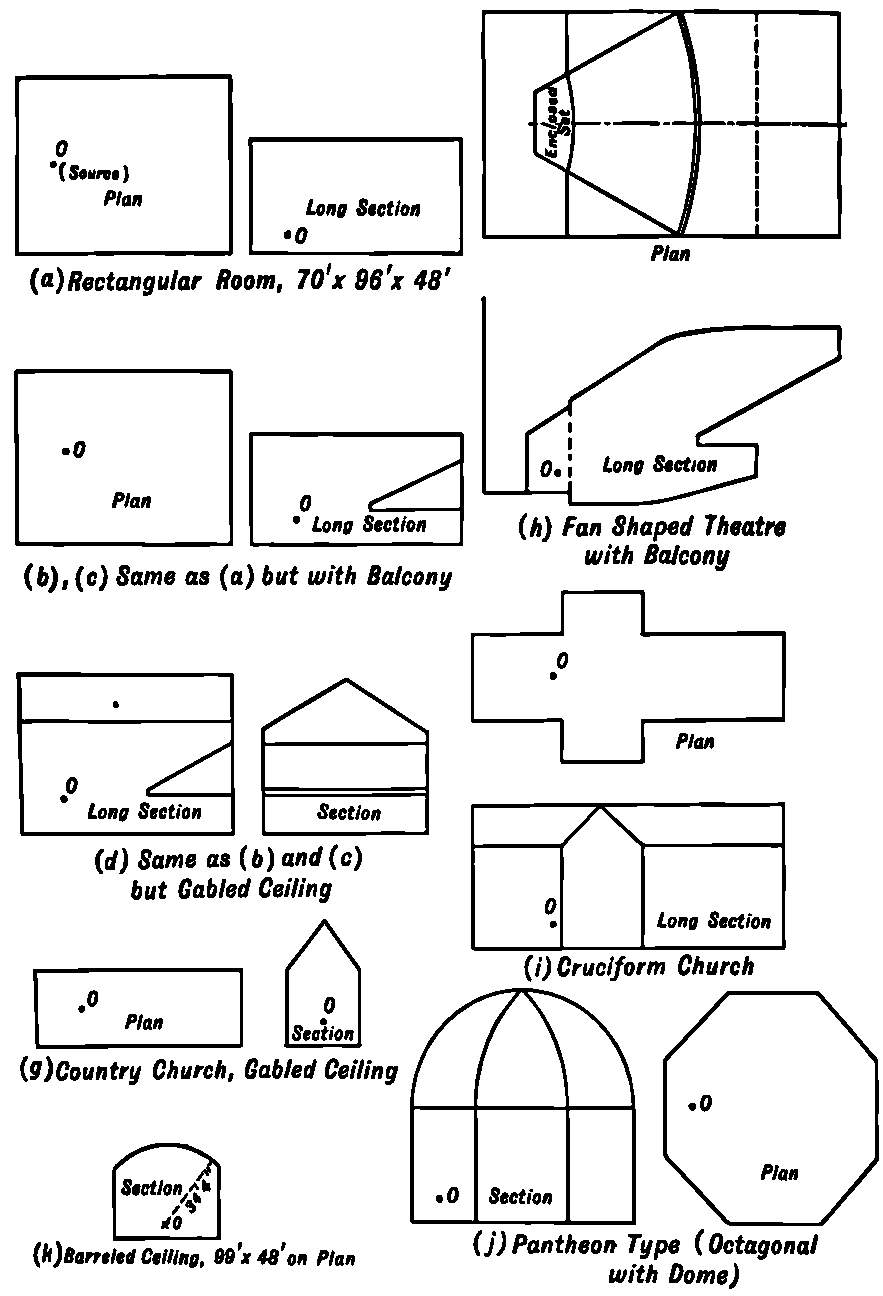
\includegraphics[width=0.5\textwidth]{archivos/mfpknudsen1.pdf}
%    \caption{Modelos utilizados para el cálculo de MFP por Vern O. Knudsen. Figura extraída del libro \cite{Knudsen1932}, pág. 140.}
%    \label{fig:knudsen1}
%\end{figure}
%\FloatBarrier
%\begin{figure}[ht]
%    \centering
%    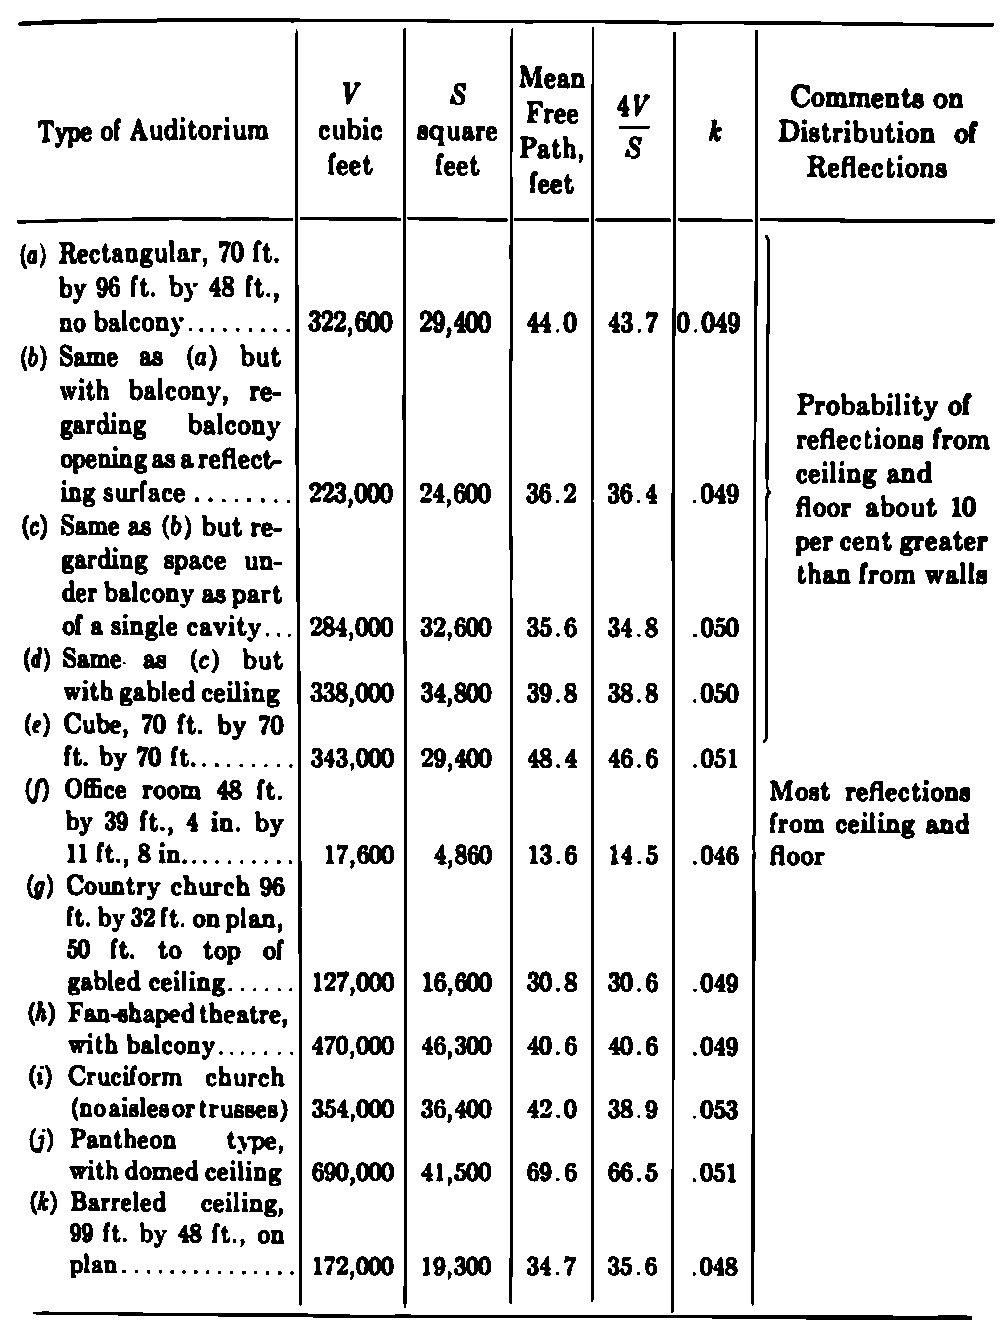
\includegraphics[width=0.5\textwidth]{archivos/mfpknudsen2.pdf}
%    \caption{Resultados obtenidos con el cálculo de MFP por Vern O. Knudsen. Tabla extraída del libro \cite{Knudsen1932}, pág. 141.}
%    \label{fig:knudsen2}
%\end{figure}
%\FloatBarrier
\begin{figure}[ht]
    \centering
    \begin{subfigure}[b]{0.48\textwidth}
    	\centering
        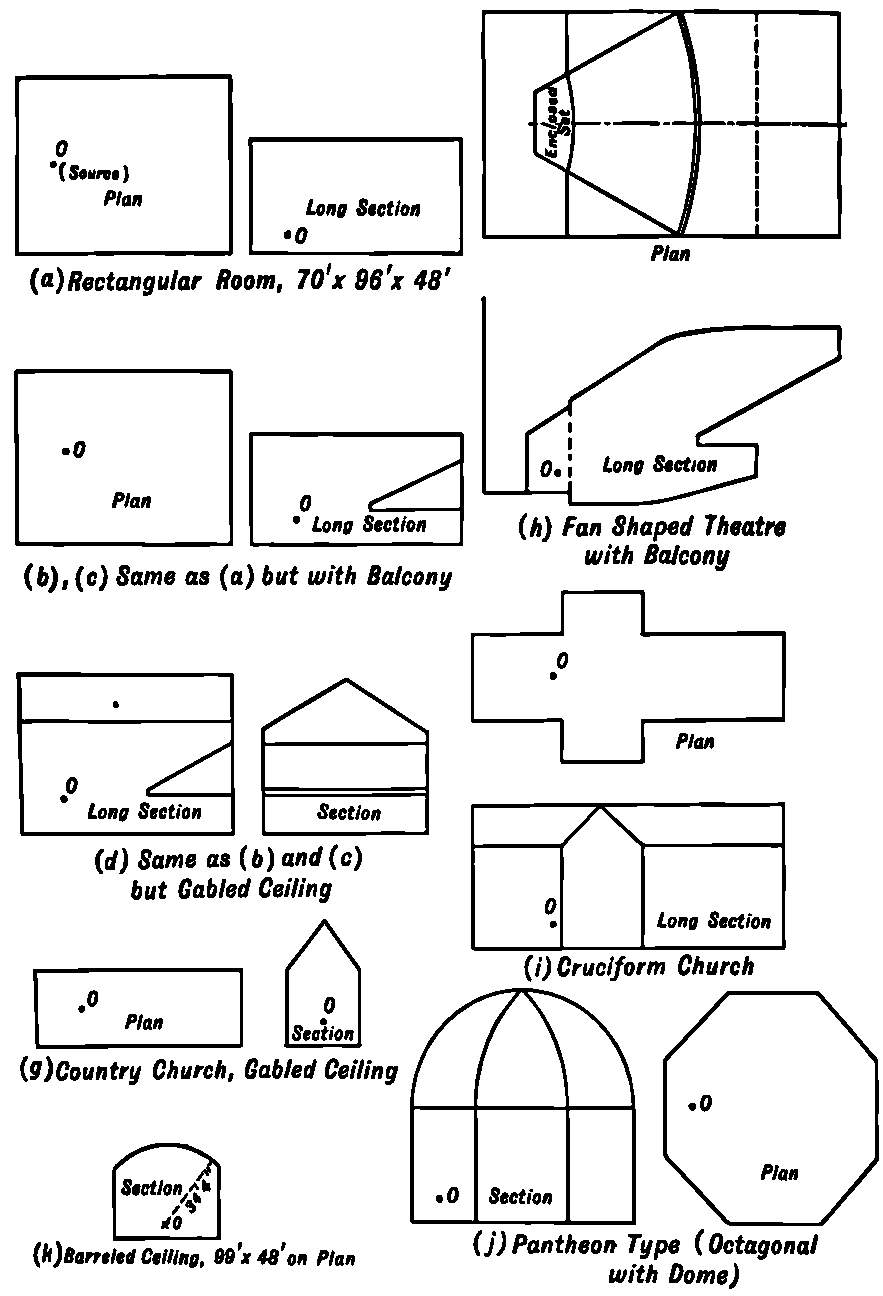
\includegraphics[width=0.9\linewidth]{archivos/mfpknudsen1.pdf}
        \caption{}
        \label{fig:knudsen1}
    \end{subfigure}
    ~ % Añadir el espacio deseado, si se deja la linea en blanco la siguiente subfigura ira en una nueva linea
    \begin{subfigure}[b]{0.48\textwidth}
    	\centering
        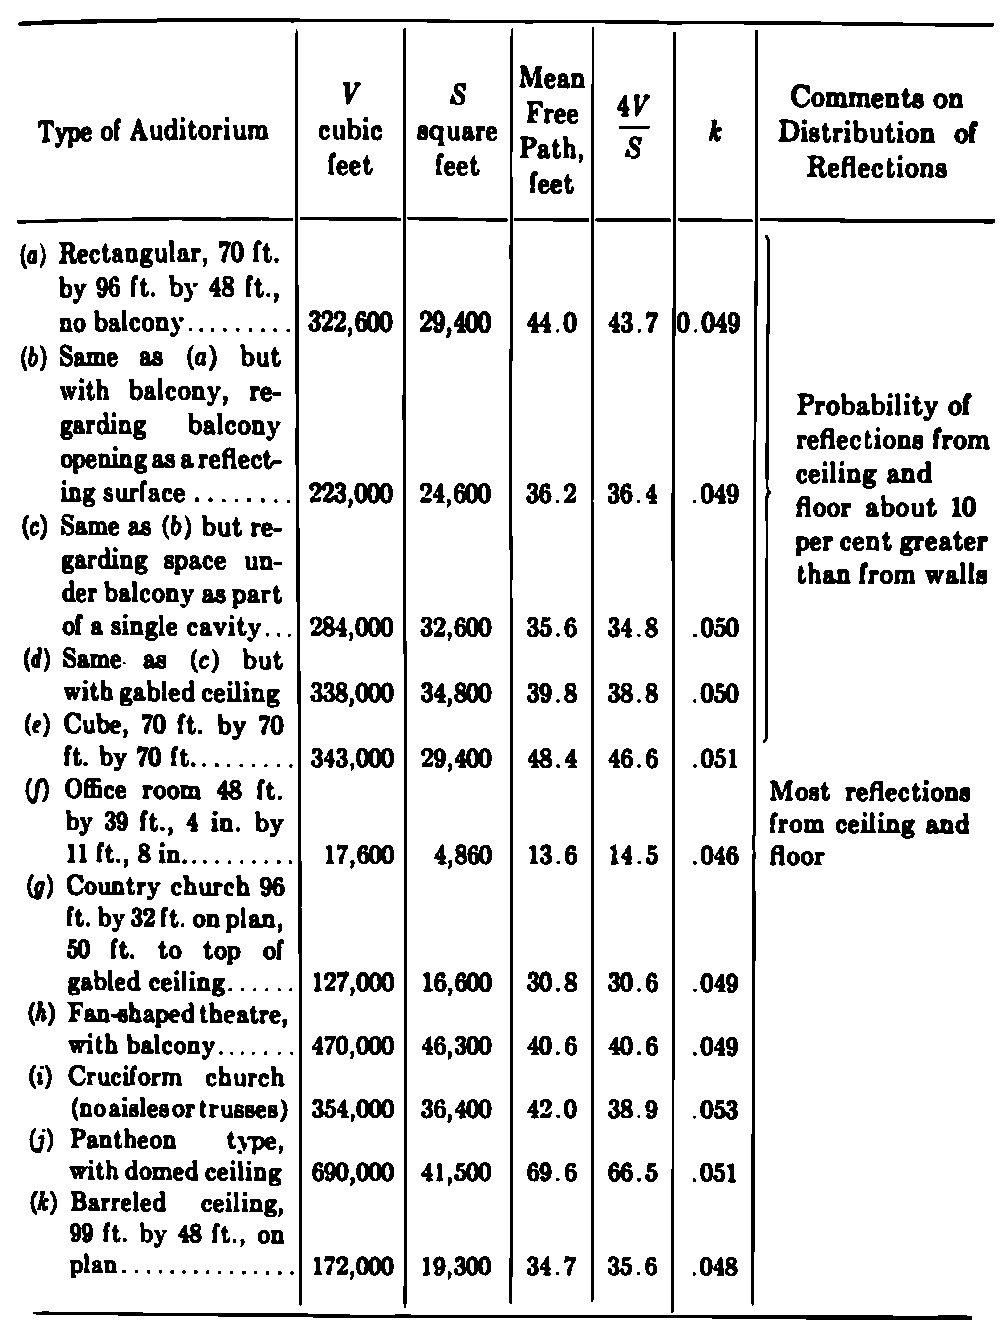
\includegraphics[width=0.9\linewidth]{archivos/mfpknudsen2.pdf}
        \caption{}
        \label{fig:knudsen2}
    \end{subfigure}
    \caption{a) Modelos utilizados para el cálculo de MFP por Vern O. Knudsen. Figura extraída del libro \cite{Knudsen1932}, pág. 140. b) Resultados obtenidos con el cálculo de MFP por Vern O. Knudsen. Tabla extraída del libro \cite{Knudsen1932}, pág. 141.}
\end{figure}
\FloatBarrier 

El factor $k$ es el valor que multiplica a $V/A$ en la ecuación del tiempo de reverberación (ecuación \ref{ecu:tr}). En la tabla (figura \ref{fig:knudsen2}) está en unidades del sistema imperial, la conversión al sistema internacional de unidades se obtiene multiplicando por la velocidad del sonido en unidades imperiales (1124 pies/s) y dividiendo por la misma velocidad en unidades métricas (343 m/s), tal que $k_\text{S.I.} = k_\text{I.}\cdot\nicefrac{1124}{343}$.

Este factor $k$ se obtiene mediante:
\begin{flalign}
	 k=l_{\mathrm{MFP}}\frac{S\ln 10^6}{ Vc}\label{factork}
\end{flalign}
\begin{condiciones}[Donde:]
	l_{\mathrm{MFP}} & \rightarrow & Es el valor de MFP experimental en metros.
\end{condiciones}


\subsection{Tiempo de reverberación}

El tiempo de reverberación se define como el tiempo que transcurre para que el nivel de presión de un sonido se reduzca 60 $dB$ (una millonésima parte) desde el instante que deja de emitirse. Siempre se expresa en segundos.

\begin{figure}[ht]
    \centering
    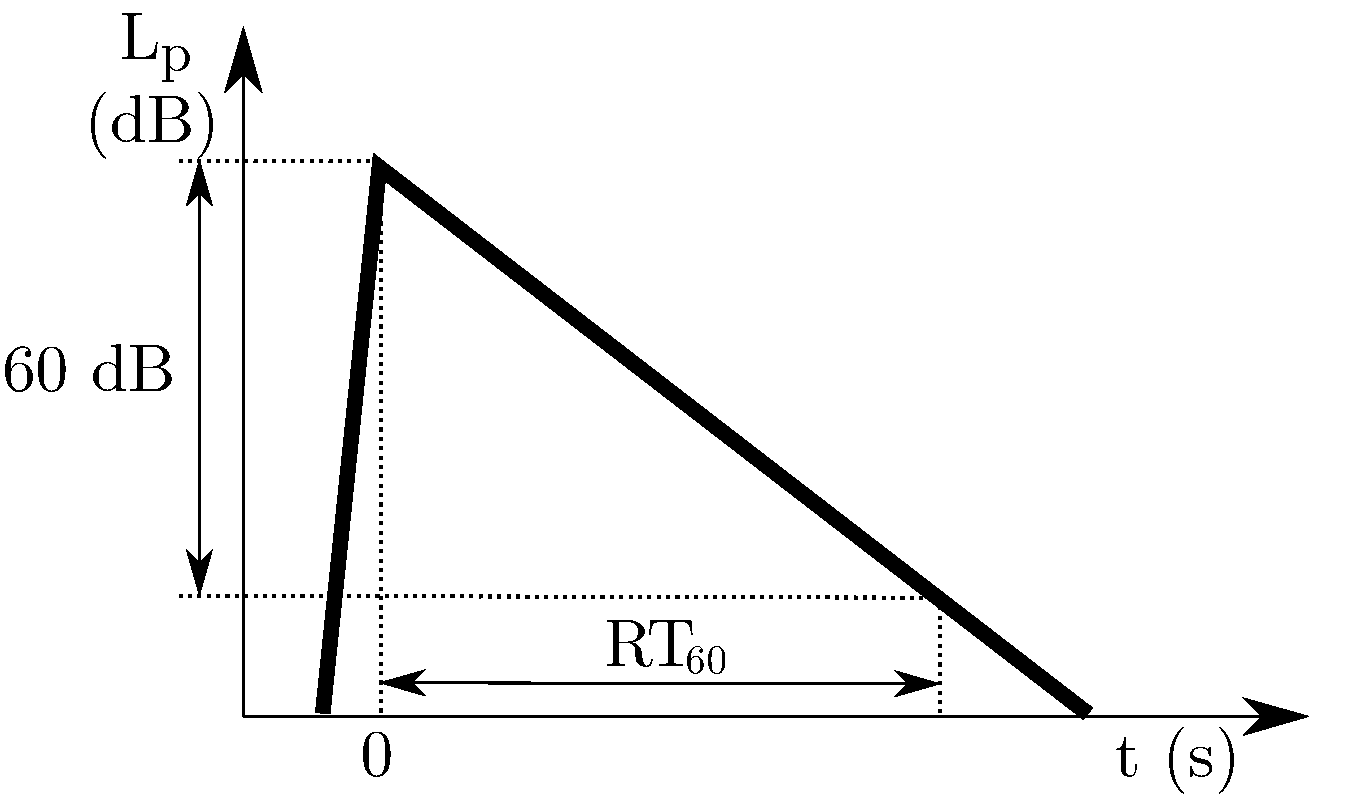
\includegraphics[width=0.4\textwidth]{archivos/tiempoRT.pdf}
    \caption{Diagrama de la definición de tiempo de reverberación.}
\end{figure}
\FloatBarrier

En la práctica es difícil medir una caída completa de 60 $dB$ por lo que es habitual utilizar:

\begin{description}
	\item [EDT:] \textit{Early Decay Time}. Es el tiempo que transcurre para que el nivel de presión se reduzca 10 $dB$ desde el instante que deja de emitirse un sonido. Tiene relación con la sensación subjetiva de la reverberación. Definido por \cite{Jordan1970}.
	\item [T20:] Es el tiempo que transcurre desde que se ha reducido 5 $dB$ hasta que se ha reducido 25 $dB$. Describe las propiedades acústicas del recinto. Definido por \cite{Atal1966}.
	\item [T30:] Es el tiempo que transcurre desde que se ha reducido 5 $dB$ hasta que se ha reducido 35 $dB$. Describe las propiedades acústicas del recinto. Definido por \cite{Atal1966}.
\end{description}

Una vez obtenido uno de estos valores se extrapola para obtener el tiempo para una caída de 60 $dB$, es decir, el EDT se multiplica por 6, el T20 por 3 y el T30 por 2. Es una práctica habitual ofrecer el valor T20 o T30 ya extrapolado.

\begin{figure}[ht]
    \centering
    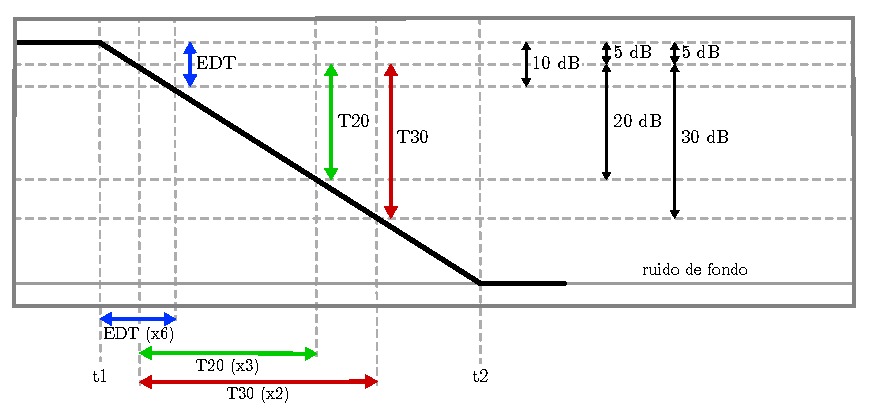
\includegraphics[width=0.8\textwidth]{archivos/EDT2030.pdf}
    \caption{Diagrama de la definición de EDT, T20 y T30.}
\end{figure}
\FloatBarrier

El cálculo teórico del tiempo de reverberación tiene en consideración la superficie, volumen y absorción del recinto. Existen en la literatura múltiples propuestas para el cálculo del tiempo de reverberación, aquí se explicarán las dos más comunes, \citeauthor{Sabine1922} y \citeauthor{Eyring1930}:

\begin{description}
	\item [Sabine:] Wallace Clement Sabine propuso su método de cálculo al final del siglo XIX que más tarde fue recogido en \textit{Collected Papers on Acoustics} \citep{Sabine1922}. Este cálculo es útil cuando el coeficiente de absorción medio $\overline{\alpha}$ se encuentra entre $0$-$0.2$ y el reparto es homogéneo, superado este valor el cálculo introduce errores mayores al 10\%.
		\begin{flalign}\label{eq:sabine}
			T = \frac{l_{\mathrm{MFP}} \ln 10^6 }{c\ \overline{\alpha}}=\frac{4 \ln 10^6\ V}{c\ S\ \overline{\alpha}}=\frac{4 \ln 10^6\ V}{c\ S\ \overline{\alpha}}\approx 0,161\frac{V}{S\ \overline{\alpha}}
		\end{flalign}
	
	\item [Eyring:] Carl Ferdinand Eyring propuso una mejora en el cálculo de \citeauthor{Sabine1922} en \cite{Eyring1930}, modificando el término de absorción total o equivalente $A$. En este caso se corrige el problema para un coeficiente mayor a $0.2$ aunque el reparto de los coeficientes debe seguir siendo homogéneo\footnote{Para un coeficiente cercano al 1 y/o  reparto de coeficientes muy extremos tanto Sabine como Eyring no son fiables, en casos como éste se debe utilizar \cite{Millington1932}.}. 
		\begin{flalign}\label{eq:eyring}
			T = \frac{l_{\mathrm{MFP}} \ln 10^6 }{-c\ \ln (1-\overline{\alpha})} = \frac{4 \ln 10^6\ V}{-c\ S \ln (1-\overline{\alpha})}\approx 0,161\frac{V}{-S \ln (1-\overline{\alpha})}
		\end{flalign}
\end{description}

Ambas ecuaciones tienen similitudes y en la literatura es habitual encontrar la ecuación del tiempo de reverberación como:
\begin{flalign}
	T =k\frac{V}{A}\approx 0,161\frac{V}{A}\label{ecu:tr}
\end{flalign}
\begin{condiciones}[Donde:]
k & \rightarrow & Constante proporcional al MFP del recinto 	(ecuación \ref{factork}).\\
A & \rightarrow & Puede ser 	$\left\{ \begin{array}{c}S\ \overline{\alpha} \quad\quad\quad\quad\;\;\; \text{Absorción equivalente de Sabine.}\\ -S \ln (1-\overline{\alpha})  \quad \text{Absorción equivalente de Eyring.}\end{array} \right.$
\end{condiciones}

\section{Parámetros de inteligibilidad y calidad acústica}

La inteligibilidad de forma genérica en la acústica se refiere a la medición de la capacidad para comprender la voz hablada. A continuación se definen algunos de los parámetros más importantes asociados a la inteligibilidad y se comentarán también algunos relacionados con la música. Existen multitud de parámetros para evaluar la inteligibilidad o la calidad acústica de un recinto, en este trabajo se exponen únicamente los desarrollados en el capítulo de resultados. Si se desea conocer muchos de estos parámetros, en \cite{Lacatis2008} se muestra un histórico de los parámetros acústicos junto a los autores y los artículos.

\subsection{Claridad C50,C80}
\label{claridad}
La claridad fue establecida por \cite{Reichardt1974} y ampliada por múltiples autores donde destaca \cite{Marshall1994}. Se define, para el caso de la palabra, como la relación entre la energía acústica recibida durante los primeros 50 milisegundos y la energía acústica después de esos 50 milisegundos, en el caso de la música el tiempo se extiende hasta los 80 milisegundos. El parámetro es adimensional y se expresa en decibelios.

Permite conocer con facilidad si predomina el campo útil sobre el campo perjudicial descritos al inicio de este capítulo. Tanto para el caso de uso para música (80 ms) como para palabra (50 ms) el cálculo general es:

\begin{flalign}
	C_t = 10\log_{10}\left( \frac{\bigints_{\;0}^{t}p^2(t)\text{d}t}{\bigints_{\;t}^{\infty}p^2(t)\text{d}t} \right)
\end{flalign}
\begin{condiciones}[Donde:]
 	t & \rightarrow & Es el periodo de integración, 50 u 80 milisegundos.\\
 	p^2 & \rightarrow & Es el valor de presión acústica al cuadrado obtenida con la respuesta al impulso (ver apartado \ref{respimpulso}).
\end{condiciones}

Este cálculo se realiza únicamente con los valores obtenidos en las bandas de octava desde 125 Hz hasta la de 4000 Hz. El valor recomendado (ISO 3382-1) para C50 debe estar comprendido entre -4dB y 4dB y para C80 entre -5dB y 5dB.
\\
\par
Además de este cálculo general es habitual el uso de los \textit{promedio} (\textit{average}). 

El C50 \textit{speech average}, definido por \cite{Marshall1994}, tiene en cuenta las bandas de octava de 500 Hz, 1000 Hz, 2000 Hz y 4000 Hz, y además incorpora una ponderación para cada una de ellas, quedando el cálculo del siguiente modo:

\begin{flalign}
	C_{50,\text{AV}} = 0.15\cdot C_{50,\text{500 Hz}} +0.25\cdot C_{50,\text{1 kHz}} + 0.35\cdot C_{50,\text{2 kHz}} + 0.25\cdot C_{50,\text{4 kHz}}
\end{flalign}

El valor recomendado para el C50 \textit{speak average} según \cite{Carrión1998} debe ser mayor a 2dB.
\\
\par 
El C80 \textit{music average} o C80(3), definido también en \cite{Marshall1994}, realiza el promedio del valor de claridad para las bandas de 500 Hz, 1000 Hz y 2000 Hz:

\begin{flalign}
	C_{80,\text{AV}} = \frac{C_{80,\text{500 Hz}}+C_{80,\text{1 kHz}}+C_{80,\text{2 kHz}}}{3}
\end{flalign}

El valor recomendado de C80(3) según \cite{beranek1986acoustics} debe estar comprendido entre -4dB y 0dB.
\\
Es posible obtener el parámetro de claridad a partir del de definición (apartado \ref{definicion}):

\begin{flalign}
	C_t = 10\log_{10}\left( \frac{D_t}{1-D_t}\right)
\end{flalign}

\subsection{Definición D50,D80}
\label{definicion}

El parámetro definición se estableció en \cite{Thiele1953}. Es similar a la claridad pero en lugar de relacionar los primeros 50 u 80 milisegundos con el resto del tiempo, se relacionan esos primeros milisegundos con el total. Del mismo modo que la claridad se tienen en cuenta las bandas de octava entre 125 Hz y 4000 Hz. 

Este parámetro es adimensional y no tiene unidades.
\vspace{-0.2cm}
\begin{flalign}
	D_t = \frac{\bigints_{\;0}^{t}p^2(t)\text{d}t}{\bigints_{\;0}^{\infty}p^2(t)\text{d}t}
\end{flalign}
\begin{condiciones}[Donde:]
 	t & \rightarrow & Es el periodo de integración, 50 u 80 milisegundos.\\
 	p^2 & \rightarrow & Es el valor de presión acústica al cuadrado obtenida con la respuesta al impulso (ver apartado \ref{respimpulso}).
\end{condiciones}

Este parámetro se puede obtener a través de la claridad operando:
\vspace{-0.2cm}
\begin{flalign}
	D_t = \frac{1}{1+10^{-\nicefrac{C_t}{10}}}
\end{flalign}

Para el D50, \cite{Arau1999} recomienda valores superiores a 0.5. En el caso del D80, dado que casi no es utilizado no hay fuentes en la literatura que recomienden valores, pero utilizando los valores de claridad C80 recomendados en la ISO 3382-1 se obtienen los valores de definición comprendidos entre 0.25 y 0.75.

\subsection{Sonoridad G}
\label{sonoridad}
La sonoridad definida en \cite{Lehmann1976} es el cociente entre el nivel recibido en un punto debido a una fuente sonora omnidireccional y el nivel que genera la misma fuente a 10 metros en campo libre. Este cálculo ofrece información sobre la ganancia acústica que produce un recinto mediante reflexiones y está inversamente relacionado con la absorción acústica del recinto. El parámetro $G$ (\textit{sound strength}) es adimensional y se expresa en escala logarítmica.

Generalmente este parámetro es utilizado en recintos para música. El cálculo tiene mayor utilidad si el recinto es lo suficientemente grande como para que la distancia entre el escenario o punto de emisión y la zona de recepción más cercana sea mayor a 10 metros. 

Este párametro se calcula como:
	\vspace{-0.2cm}
	\begin{flalign}
		G = 10\log_{10}\left( \frac{\bigints_{\;0}^{\infty} p^2(t) \text{d}t}{\bigints_{\;0}^{\infty} p^2_{10m}(t) \text{d}t} \right)= L_p - L_{p,10m}
	\end{flalign} 

En \cite{Beranek2011} se recomienda un valor entre 4 dB y 7.5 dB para la $G_{mid}$ que se refiere al parámetro $G$ teniendo en cuenta únicamente las bandas de frecuencia de 500 Hz y 1000 Hz. 



\subsection{Índice de articulación AI}
\label{indicearticulacion}
El índice de articulación es una herramienta que permite conocer la cantidad de habla que puede percibir un receptor, definido por \cite{French1947} y ampliamente desarrollado por \cite{Kryter1962}, asignando unos pesos a cada banda de frecuencia de la relación señal ruido recibida. Estos pesos están definidos por \citeauthor{Kryter1962} para tercios de octava, bandas de octava y bandas de octava habituales (de 250 Hz a 4000 Hz), aquí se va a definir el cálculo para el caso de bandas de octava habituales:

\begin{flalign}
	AI = \sum\limits_{i=1}^{5} W_iR_i
\end{flalign}

\begin{condiciones}[Donde:]
	i & \rightarrow & Es el índice de la banda de octava (250 Hz, 500 Hz, 1 kHz, 2 kHz y 4 kHz).\\
	W_i & \rightarrow & Es el peso para cada banda de frecuencia, indicado en la tabla \ref{pesosai}.\\
	R_i & \rightarrow & Es la relación señal ruido para cada banda de frecuencia en dB.
\end{condiciones}

\begin{table}[ht]
\centering
{\scalefont{0.9}
\begin{tabular}{@{}lccccc@{}}
\toprule
Frecuencia (Hz) & 250 & 500 & 1000 & 2000 & 4000 \\ \midrule
Peso $W$ & 0.0018 & 0.0050 & 0.0075 & 0.0107 & 0.0083 \\ \bottomrule
\end{tabular}
}
\caption{Peso de cada banda de octava para el cálculo de AI.}
\label{pesosai}
\end{table}
\FloatBarrier

El valor comprende entre 0 y 1, donde 0 es el valor correspondiente al nulo entendimiento del habla y 1 al completo entendimiento de éste.

\citeauthor{Kryter1962} también define una corrección del AI debido al tiempo de reverberación del recinto representado por la curva de la figura \ref{graf:correcionai}.

\begin{figure}[ht]
    \centering
    {\scalefont{0.8}
    %%%%%%%%%%%%%%%%%%%%%%%%%%%%%%%%%%%%%%%%%%%%%%%%%%%%%%%%%%%%%%%%%%%%%%%%
% Escuela Politécnica Superior de la Universidad de Alicante
% Realizado por: Jose Manuel Requena Plens
% Contacto: info@jmrplens.com / Telegram:@jmrplens
%%%%%%%%%%%%%%%%%%%%%%%%%%%%%%%%%%%%%%%%%%%%%%%%%%%%%%%%%%%%%%%%%%%%%%%%

\definecolor{mycolor1}{rgb}{0.00000,0.44700,0.74100}%
%
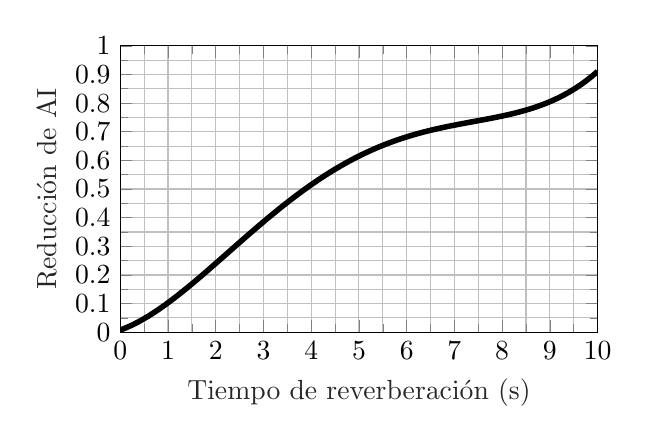
\begin{tikzpicture}

\begin{axis}[%
width=0.5\textwidth,
height=0.3\textwidth,
at={(0\textwidth,0\textwidth)},
scale only axis,
xmin=0,
xmax=10,
xlabel style={font=\color{white!15!black}},
xlabel={Tiempo de reverberación (s)},
xtick distance=1,
minor x tick num= 1,
minor y tick num= 1,
ymin=0,
ymax=1,
ytick distance=0.1,
grid=both,
ylabel style={font=\color{white!15!black}},
ylabel={Reducción de AI},
axis background/.style={fill=white},
legend style={legend cell align=left, align=left, draw=white!15!black}
]

\addplot[color=black,line width=2.0pt,domain=0:10, samples=85]{0.0004264*x^4 -0.008245*x^3 + 0.04282*x^2 + 0.06021*x + 0.007629};
\end{axis}
\end{tikzpicture}%
    }
    \caption{Valores de corrección de AI según tiempo de reverberación.}
    \label{graf:correcionai}
\end{figure}
\FloatBarrier

Este parámetro da pie a crear un índice buscando el efecto contrario, zonas donde la privacidad de la conversación sea máxima, este índice de privacidad se calcula como:
\begin{flalign}
	PI = 1 - AI
\end{flalign}

Teniendo privacidad máxima con un índice igual a 0, y ninguna privacidad con un valor igual a 1.

\section{Teoría de campos acústicos}

La teoría de los campos acústicos aplicada en este trabajo es la desarrollada en el apartado \ref{teoriarevisadacorregida}, denominada \textit{teoría revisada corregida}. A continuación se muestran los antecedentes del cálculo de los campos acústicos.

\subsection{Campos directo y reverberado}

El campo directo por definición es el campo generado por las ondas sonoras que no han sufrido reflexiones, mientras que el campo reverberado es el campo generado por las ondas sonoras que han sufrido al menos una reflexión. Habitualmente el campo reverberado se descompone en campo temprano y campo tardío (\textit{early field} y \textit{late field}). También se puede denominar reflexión temprana y tardía o primeras reflexiones y cola reverberante.

%\begin{figure}[ht]
%    \centering
%    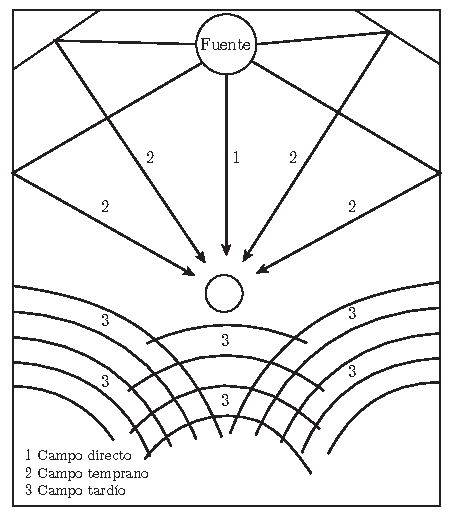
\includegraphics[width=0.4\textwidth]{archivos/campos.pdf}
%    \caption{Descripción de los campos acústicos. Figura extraída y modificada de \cite{Self2009}, pág. 111.}
%    \label{descampos}
%\end{figure}
\begin{figure}[ht]
    \centering
    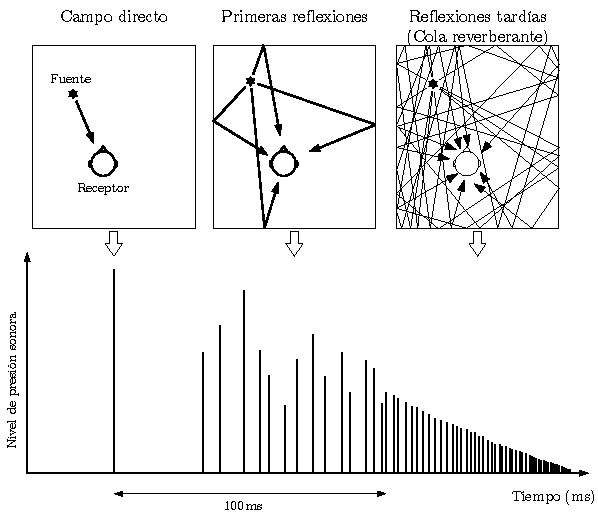
\includegraphics[width=0.65\textwidth]{archivos/campos2.pdf}
    \caption{Ecograma asociado a un receptor con indicación del campo directo, las primeras reflexiones y la cola reverberante. Figura extraída de \cite{Carrión1998}, pág. 50.}
    \label{ecograma}
\end{figure}
Un ecograma (figura \ref{ecograma}) muestra el nivel y tiempo de llegada de cada rayo sonoro a un receptor, facilitando la representación de los campos acústicos en el receptor.
En la práctica es relativamente sencillo desglosar la historia temporal (campo directo, primeras reflexiones y cola reverberante), se suele separar la pendiente en $\Delta t$ para separar el campo en un símil de rayos acústicos. Habitualmente se separa en incrementos de 1 milisegundo.

\par Para el cálculo teórico se ha escrito mucho pero existe una teoría sobradamente aceptada; es la propuesta de \cite{Hopkins1948} que describe el campo acústico total como la suma del campo directo y el campo reverberado, que años más tarde fue modificada por \cite{davis1984}. Este cálculo asume que el campo reverberante es estacionario, es decir, constante en cualquier punto del recinto.

\begin{flalign}
	I =& \frac{WQ}{4\pi r^2} + \frac{4W}{A}\label{eq:hopkins}
\end{flalign}
\begin{condiciones}[Donde:]
	I & \rightarrow & Es la intensidad acústica total en $W/m^2$.\\
	r & \rightarrow & Es la distancia emisor-receptor en metros.\\
	A & \rightarrow & Es la absorción equivalente de Sabine o Eyring.
\end{condiciones}

El término $\nicefrac{WQ}{4\pi r^2}$ corresponde a la intensidad del campo directo a distancia $r$ de la fuente y el término $\nicefrac{4W}{A}$ corresponde a la intensidad del campo reverberado que, como se puede observar, presupone que es constante en cualquier punto del recinto.

\begin{figure}[ht]
    \centering
    {\scalefont{0.8}
    %%%%%%%%%%%%%%%%%%%%%%%%%%%%%%%%%%%%%%%%%%%%%%%%%%%%%%%%%%%%%%%%%%%%%%%%
% Escuela Politécnica Superior de la Universidad de Alicante
% Realizado por: Jose Manuel Requena Plens
% Contacto: info@jmrplens.com / Telegram:@jmrplens
%%%%%%%%%%%%%%%%%%%%%%%%%%%%%%%%%%%%%%%%%%%%%%%%%%%%%%%%%%%%%%%%%%%%%%%%

\definecolor{mycolor1}{rgb}{0.60000,0.00000,0.60000}%
%
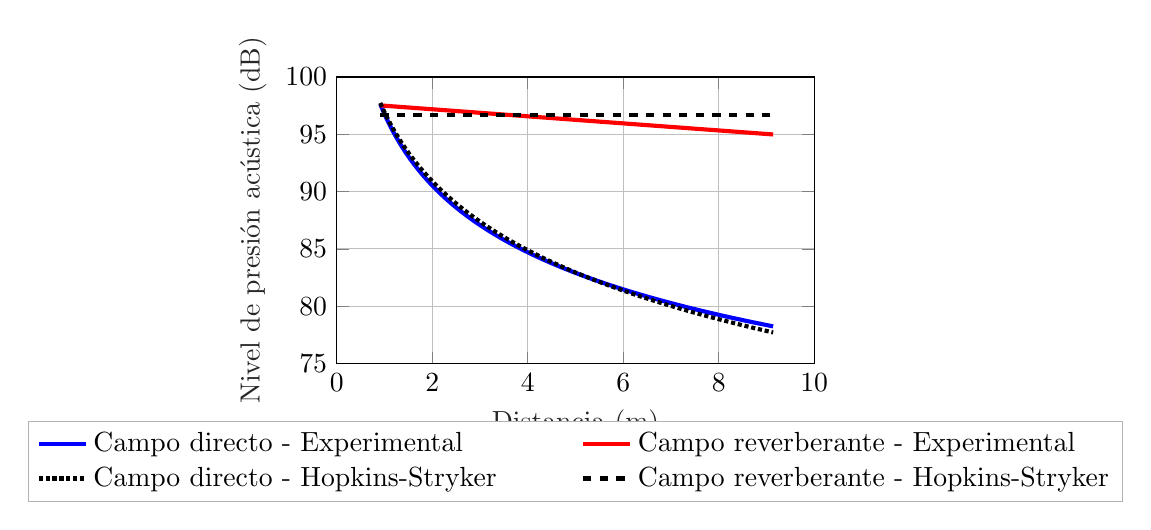
\begin{tikzpicture}

\begin{axis}[%
width=0.5\textwidth,
height=0.3\textwidth,
at={(0\textwidth,0\textwidth)},
scale only axis,
xmin=0,
xmax=10,
xlabel style={font=\color{white!15!black}},
xlabel={Distancia (m)},
ymin=75,
ymax=100,
ytick distance=5,
ylabel style={font=\color{white!15!black}},
ylabel={Nivel de presión acústica (dB)},
axis background/.style={fill=white},
xmajorgrids,
ymajorgrids,
legend style={at={(0.5,-0.03)}, anchor=north, legend cell align=left, align=left, draw=white!15!black},
legend columns = 2,legend style={at={(0.5,-0.2)}, anchor=north, legend cell align=left, align=left, draw=white!70!black, /tikz/every even column/.append style={column sep=1.0cm}}
]
\addplot [color=blue,line width=1.5pt]
  table[row sep=crcr]{%
0.911043357914437	97.6380061935451\\
0.971043357914425	97.0416130715755\\
1.03104335791443	96.484310473315\\
1.10104335791443	95.8774048250365\\
1.17104335791443	95.3113917575971\\
1.24104335791444	94.7813060660669\\
1.31104335791443	94.2830244776188\\
1.38104335791444	93.8130865478216\\
1.46104335791443	93.3069806543866\\
1.54104335791443	92.8303775474136\\
1.62104335791443	92.3801537924959\\
1.70104335791443	91.9536509875259\\
1.78104335791443	91.5485883526324\\
1.87104335791443	91.1160767261982\\
1.96104335791443	90.7057903345106\\
2.05104335791444	90.3156426154386\\
2.14104335791443	89.9438239896602\\
2.23104335791443	89.5887552104351\\
2.33104335791442	89.2121989170647\\
2.43104335791443	88.8529466109456\\
2.53104335791443	88.5095386461936\\
2.63104335791444	88.1806902279387\\
2.74104335791444	87.8344205548337\\
2.85104335791443	87.5030577659302\\
2.96104335791443	87.1854208783258\\
3.07104335791443	86.8804620884833\\
3.18104335791443	86.5872475992273\\
3.30104335791444	86.2797919676868\\
3.42104335791443	85.9843498413856\\
3.54104335791443	85.7000543544441\\
3.66104335791444	85.426127966722\\
3.79104335791443	85.1402654198586\\
3.92104335791443	84.8649508844128\\
4.05104335791444	84.5994642356986\\
4.18104335791443	84.3431556826281\\
4.32104335791443	84.0767218124595\\
4.46104335791443	83.8195859804349\\
4.60104335791443	83.5711467621151\\
4.75104335791443	83.3139935284142\\
4.90104335791443	83.0655890600581\\
5.05104335791444	82.8253812483105\\
5.20104335791443	82.5928679479935\\
5.36104335791443	82.3528195444158\\
5.52104335791444	82.120498287441\\
5.68104335791443	81.8954420472253\\
5.85104335791443	81.6638082159739\\
6.02104335791444	81.4394362677818\\
6.19104335791442	81.2219029078978\\
6.37104335791443	80.9985968064552\\
6.55104335791444	80.7821012050116\\
6.74104335791444	80.5605400646246\\
6.93104335791443	80.3457203545647\\
7.12104335791443	80.1372603842554\\
7.32104335791443	79.9243144622446\\
7.52104335791444	79.7176514144308\\
7.73104335791443	79.5070397973059\\
7.94104335791442	79.3026073677421\\
8.15104335791443	79.1040164504568\\
8.37104335791443	78.9018955433603\\
8.59104335791443	78.7055148221739\\
8.82104335791443	78.5060156380693\\
9.05104335791444	78.3121381646318\\
9.14104335791443	78.2377385102596\\
};
\addlegendentry{Campo directo - Experimental}

\addplot [color=red,line width=1.5pt]
  table[row sep=crcr]{%
0.911043357914437	97.5218752230605\\
9.14104335791443	94.9864450736265\\
};
\addlegendentry{Campo reverberante - Experimental}

\addplot [color=black, densely dotted, line width=1.5pt]
  table[row sep=crcr]{%
0.911043357914437	97.7331926631792\\
0.971043357914425	97.1792011477379\\
1.04104335791443	96.5745972347531\\
1.11104335791443	96.0093534389856\\
1.18104335791443	95.4786567564759\\
1.25104335791443	94.9785263574731\\
1.33104335791442	94.4401295353534\\
1.41104335791444	93.9331664115882\\
1.49104335791444	93.4541681380115\\
1.57104335791443	93.0002101682137\\
1.65104335791443	92.5688040192524\\
1.74104335791444	92.1077818536397\\
1.83104335791442	91.67000102226\\
1.92104335791443	91.253230247119\\
2.01104335791443	90.8555449059847\\
2.11104335791443	90.4340305227801\\
2.21104335791443	90.0320284059368\\
2.31104335791443	89.6478117182375\\
2.41104335791444	89.2798731791945\\
2.52104335791444	88.892367288714\\
2.63104335791444	88.5214134861318\\
2.74104335791444	88.1656554813739\\
2.85104335791443	87.8238971470306\\
2.97104335791443	87.4657937924312\\
3.09104335791443	87.121871648269\\
3.21104335791443	86.7910501914252\\
3.33104335791442	86.4723678740925\\
3.46104335791443	86.1398327886619\\
3.59104335791443	85.8195606111837\\
3.72104335791443	85.5106789771931\\
3.85104335791443	85.2124054217199\\
3.99104335791444	84.9022446689407\\
4.13104335791444	84.602778523021\\
4.27104335791444	84.3132939822976\\
4.41104335791444	84.033147053859\\
4.56104335791443	83.7426895724501\\
4.71104335791443	83.4616315615413\\
4.86104335791443	83.1893836916001\\
5.02104335791444	82.9080941543875\\
5.18104335791443	82.635629052434\\
5.34104335791443	82.3714515163175\\
5.51104335791443	82.0992970302704\\
5.68104335791443	81.8354115101393\\
5.85104335791443	81.5793072595462\\
6.03104335791443	81.3161245733647\\
6.21104335791443	81.0606823675505\\
6.39104335791443	80.8125383092309\\
6.58104335791442	80.5580785454699\\
6.77104335791444	80.3108616913113\\
6.96104335791443	80.0704868101745\\
7.16104335791444	79.8244475218628\\
7.36104335791443	79.585186070651\\
7.57104335791443	79.3408589206871\\
7.78104335791443	79.1032168805553\\
7.99104335791444	78.8719038454604\\
8.21104335791443	78.6360066789118\\
8.43104335791443	78.4063471322951\\
8.66104335791444	78.1725693325264\\
8.89104335791443	77.9449190244605\\
9.13104335791444	77.7135654870847\\
9.14104335791443	77.704058208972\\
};
\addlegendentry{Campo directo - Hopkins-Stryker}

\addplot [color=black, dashed, line width=1.5pt]
  table[row sep=crcr]{%
0.911043357914437	96.7131831634935\\
9.14104335791443	96.7131831634935\\
};
\addlegendentry{Campo reverberante - Hopkins-Stryker}



\end{axis}
\end{tikzpicture}%
    }
    \caption{Comparación de los campos acústicos obtenidos experimentalmente y mediante la ecuación Hopkins-Stryker. El tiempo de integración del experimental es 0-1 ms para el campo directo y 1-$\infty$ para el campo reverberante.}
    \label{graf:hopkinsstryker}
\end{figure}

Se ha comprobado empíricamente que el término de campo directo corresponde aproximadamente al espacio temporal de 0 a 1ms\footnote{Esta afirmación es válida cuando los datos son ideales temporalmente hablando, tal como los ofrece un programa de simulación acústica, en la práctica el espacio temporal del campo directo fluctúa entre los 2 y los 10 milisegundos.\label{unmilisegundo}} de un ecograma y el término del campo reverberado corresponde aproximadamente al espacio temporal desde 1ms a infinito (figura \ref{graf:hopkinsstryker}). 

\subsubsection{Distancia crítica}

La distancia crítica se define como la distancia donde el campo directo y el reverberado se cruzan, a partir de este punto el campo reverberante predomina sobre el campo directo y se indica como una zona de baja inteligibilidad. Esto no es correcto, estando comprobado empíricamente que esta distancia no se aproxima a la zona donde la inteligibilidad se reduce.

El cálculo de la distancia crítica es una función derivada de la ecuación Hopkins-Stryker \ref{eq:hopkins}, se puede obtener fácilmente igualando los términos de ambos campos y despejando la distancia, así se obtiene la distancia donde el valor de los campos es el mismo.

\begin{flalign*}
	&& \frac{WQ}{4\pi D_c^2} &= \frac{4W}{A} &&\\
	&& \frac{Q}{4\pi D_c^2} &= \frac{4}{A} &&
\end{flalign*}
\begin{flalign}
	D_c = \sqrt{\frac{QA}{16\pi}}
\end{flalign}
\begin{condiciones}[Donde:]
	D_c & \rightarrow & Es la distancia crítica en metros.\\
	A & \rightarrow & Es la absorción equivalente de Sabine o Eyring.
\end{condiciones}

\subsection{Teoría revisada o moderna}
\label{teoriarevisada}

La \textit{teoría revisada} o \textit{teoría moderna} es una mejora del cálculo de campos acústicos propuesta por \cite{Barron1988} y ampliada en \cite{Barron2015}, en la que se describe mejor el comportamiento de los mismos. En esta \textit{teoría revisada} el campo reverberante ya no se considera estacionario o constante sino que tiene una pendiente respecto a la distancia, además permite obtener los campos acústicos definiendo un tiempo de integración para los diferentes campos.

El campo total se calcula como:
\begin{flalign*}
	I_0^\infty (r,t)&= \frac{WQ}{4\pi r^2} + \frac{4W}{A} 10^{-\left(\frac{60t}{10T} \right)}\\
	I_0^\infty (r,t)&= \frac{WQ}{4\pi r^2} + \frac{4W}{A} e^{-\left(\frac{6\ln(10)t}{T} \right)}\\
\end{flalign*}
\vspace{-1cm}
\begin{flalign}
	I_0^\infty (r,t)&= \frac{WQ}{4\pi r^2} + \frac{4W}{A} e^{-\left(\frac{13,82t}{T} \right)}\label{eq:barronT}
\end{flalign}
\begin{condiciones}[Donde:]
	I_0^\infty & \rightarrow & Es la intensidad acústica total en $W/m^2$. Desde 0 milisegundos a infinito (fin de la cola reverberante).\\
	r & \rightarrow & Es la distancia emisor-receptor en metros.\\
	t & \rightarrow & Es el tiempo que tarda el sonido desde el emisor al receptor en segundos.\\
	T & \rightarrow & Es el tiempo de reverberación.\\
	A & \rightarrow & Es la absorción equivalente de Sabine o Eyring.
\end{condiciones}
El tiempo $t$ se puede sustituir por $r/c$ para que en lugar de estar en función del tiempo y la distancia se calcule sólo en función de la distancia emisor-receptor ($r=$ distancia ; $c=$ velocidad del sonido en el aire).


La ecuación permite obtener el campo de primeras reflexiones y el de cola reverberante por separado a partir del término de campo reverberante incluido en la ecuación \ref{eq:barronT} (segundo sumando). Con ello es posible redefinir los campos como \textit{campo útil} (0 - $t_0$) y \textit{campo perjudicial} ($t_0$ - $\infty$). El campo útil incluye el campo directo y el campo temprano; y el campo perjudicial el campo reverberante. Para obtener el campo temprano se realiza la diferencia entre el total del campo reverberante (segundo sumando de la ecuación anterior) y el campo a partir de cierto tiempo de integración (campo reverberante), obteniendo así el campo entre 1 milisegundo y $t_0$ también denominado temprano o \textit{early}. 


\begin{flalign}
	I_L = I_t^\infty (r)&= \frac{4W}{A} e^{-\left(\frac{13,82\left(\frac{r}{c}+t_0\right)}{T}\right)}\\
	I_E = I_1^t (r)&= \frac{4W}{A} \left(e^{-\left(\frac{13,82\frac{r}{c}}{T}\right)} - e^{-\left(\frac{13,82\left(\frac{r}{c}+t_0\right)}{T}\right)}\right)\label{tempranobarron}
\end{flalign}
\begin{condiciones}[Donde:]
	I_t^\infty & \rightarrow & Es la intensidad del campo tardío o cola reverberante (\textit{Late}) en $W/m^2$ desde el tiempo $t_0$ a infinito. Este campo pasa a denominarse \textit{campo perjudicial}.\\
	I_1^t & \rightarrow & Es la intensidad del campo temprano o primeras reflexiones (\textit{Early}) en $W/m^2$ desde 1 ms a $t_0$. No tiene en cuenta el campo directo que ocupa el espacio temporal de 0 a 1 milisegundo\textsuperscript{\ref{unmilisegundo}}.\\
	t_0 & \rightarrow & Es el tiempo de integración, en segundos, donde terminan las primeras reflexiones y comienza la cola reverberante. En recintos para palabra el tiempo son 50 milisegundos y para música 80 milisegundos \citep{Haas1949}.
\end{condiciones}

Por lo que el cálculo general de la teoría revisada para el campo útil y el campo perjudicial se calculan como:

\begin{flalign}
	I_t^\infty (r)&= \frac{4W}{A} e^{-\left(\frac{13,82\left(\frac{r}{c}+t_0\right)}{T}\right)}\\
	I_0^t (r)&= \frac{WQ}{4\pi r^2} + \frac{4W}{A} \left(e^{-\left(\frac{13,82\frac{r}{c}}{T}\right)} - e^{-\left(\frac{13,82\left(\frac{r}{c}+t_0\right)}{T}\right)}\right)
\end{flalign}
\begin{condiciones}[Donde:]
	I_0^t & \rightarrow & Es la intensidad del campo útil en $W/m^2$ para el tiempo de integración de 0 a $t_0$.\\
	I_t^\infty & \rightarrow & Es la intensidad del campo perjudicial en $W/m^2$ para el tiempo de integración de $t_0$ a infinito.
\end{condiciones}


También es posible obtener directamente el nivel de presión acústica teniendo en cuenta la ecuación \ref{eq:intensidadimpedancia} y \ref{eq:nivelpresion}:

\begin{flalign}
	L_p{_t^\infty} (r)&= 10\log_{10} \left[\frac{Z}{p_0^2} \left(\frac{4W}{A} e^{-\left(\frac{13,82\left(\frac{r}{c}+t_0\right)}{T}\right)}\right)\right]\label{eq:barron1}\\
	L_p{_0^t} (r)&= 10\log_{10} \left[\frac{Z}{p_0^2} \left(\frac{WQ}{4\pi r^2} +\frac{4W}{A} \left(e^{-\left(\frac{13,82\frac{r}{c}}{T}\right)} -e^{-\left(\frac{13,82\left(\frac{r}{c}+t_0\right)}{T}\right)}\right)\right)\right]\label{eq:barron2}
\end{flalign}

Como curiosidad, \cite{Barron1988} proponen introducir la potencia acústica en picovatios ($10^{-12}$), con ello el término $Z/p_o^2 \approx 10^{12}$ se anula. Esta simplificación introduce una pérdida aproximada del 3\% de intensidad acústica, por lo que la simplificación no se utilizará.

Se ha comparado la \textit{teoría revisada} de \cite{Barron1988} con los resultados obtenidos experimentalmente (figura \ref{graf:barron}) y siguen sin ajustarse al comportamiento real de un recinto; las pendientes son similares pero los niveles absolutos no se ajustan, por lo que el punto de cruce o distancia crítica obtenida con la \textit{teoría revisada} no es correcta.

\begin{figure}[ht]
    \centering
    {\scalefont{0.8}
    %%%%%%%%%%%%%%%%%%%%%%%%%%%%%%%%%%%%%%%%%%%%%%%%%%%%%%%%%%%%%%%%%%%%%%%%
% Escuela Politécnica Superior de la Universidad de Alicante
% Realizado por: Jose Manuel Requena Plens
% Contacto: info@jmrplens.com / Telegram:@jmrplens
%%%%%%%%%%%%%%%%%%%%%%%%%%%%%%%%%%%%%%%%%%%%%%%%%%%%%%%%%%%%%%%%%%%%%%%%

\definecolor{mycolor1}{rgb}{0.60000,0.00000,0.60000}%
%
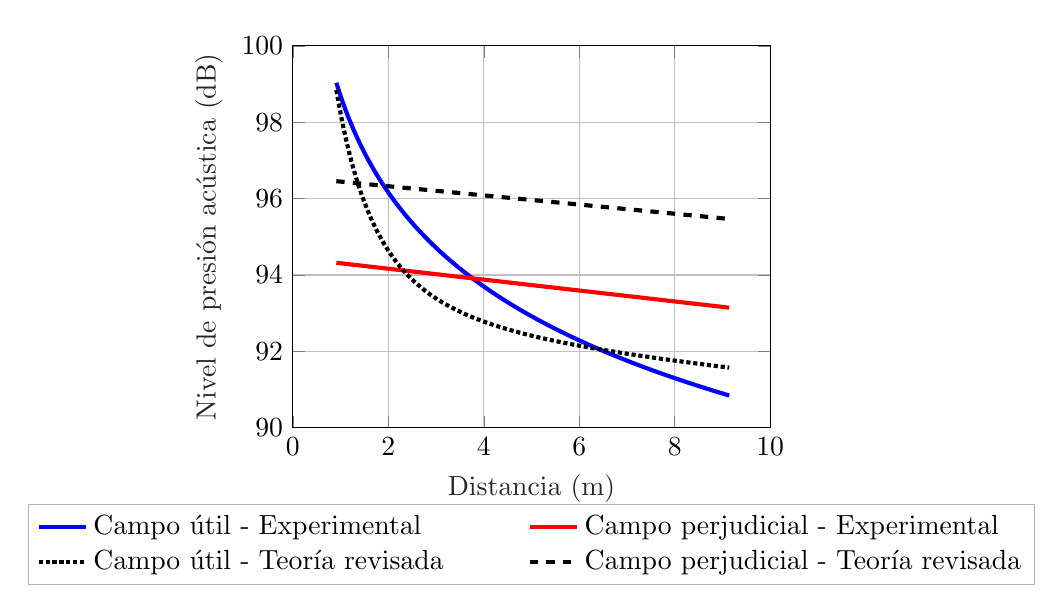
\begin{tikzpicture}

\begin{axis}[%
width=0.5\textwidth,
height=0.4\textwidth,
at={(0\textwidth,0\textwidth)},
scale only axis,
xmin=0,
xmax=10,
xlabel style={font=\color{white!15!black}},
xlabel={Distancia (m)},
ymin=90,
ymax=100,
ylabel style={font=\color{white!15!black}},
ylabel={Nivel de presión acústica (dB)},
axis background/.style={fill=white},
xmajorgrids,
ymajorgrids,
legend style={at={(0.5,-0.03)}, anchor=north, legend cell align=left, align=left, draw=white!15!black},
legend columns = 2,legend style={at={(0.5,-0.2)}, anchor=north, legend cell align=left, align=left, draw=white!70!black, /tikz/every even column/.append style={column sep=1.0cm}}
]

\addplot [color=blue,line width=1.5pt]
  table[row sep=crcr]{%
0.911043357914437	99.0320903003883\\
0.971043357914425	98.7959528580098\\
1.04104335791443	98.5388845359429\\
1.11104335791443	98.2991565611425\\
1.18104335791443	98.0746113747233\\
1.25104335791443	97.8634686967113\\
1.33104335791442	97.6366789189634\\
1.41104335791444	97.4236104651384\\
1.49104335791444	97.2227224106986\\
1.57104335791443	97.0327183901271\\
1.66104335791444	96.8306093715308\\
1.75104335791443	96.6395556707976\\
1.84104335791443	96.4584289152229\\
1.93104335791443	96.2862642660283\\
2.03104335791443	96.1044739711391\\
2.13104335791444	95.9317415415692\\
2.23104335791443	95.7672211044658\\
2.34104335791443	95.5948612142661\\
2.45104335791443	95.4307062204238\\
2.56104335791443	95.2740225949879\\
2.68104335791443	95.1108663553771\\
2.80104335791444	94.9551165840878\\
2.92104335791443	94.806140571678\\
3.05104335791444	94.6517513929231\\
3.18104335791443	94.5040410792525\\
3.32104335791443	94.3518142639458\\
3.46104335791443	94.2061042231499\\
3.60104335791443	94.0663847075716\\
3.75104335791443	93.9228053201509\\
3.90104335791443	93.7850628689417\\
4.06104335791443	93.6440668175321\\
4.22104335791443	93.5087197458185\\
4.39104335791443	93.3706251877107\\
4.56104335791443	93.237969212078\\
4.74104335791444	93.1029881074567\\
4.92104335791443	92.9732220826459\\
5.11104335791443	92.8414835983793\\
5.31104335791443	92.7081906576988\\
5.51104335791443	92.5800064516834\\
5.72104335791443	92.4505060443611\\
5.94104335791442	92.3200245358077\\
6.16104335791444	92.194462292896\\
6.39104335791443	92.0680713703988\\
6.63104335791444	91.9411199156829\\
6.88104335791444	91.8138503478675\\
7.14104335791443	91.6864807854776\\
7.40104335791443	91.5638340591942\\
7.67104335791443	91.4411133083876\\
7.95104335791443	91.3184925375982\\
8.24104335791444	91.196127426742\\
8.54104335791443	91.0741566576816\\
8.85104335791443	90.9527032209901\\
9.14104335791443	90.8430159904712\\
};
\addlegendentry{Campo útil - Experimental}

\addplot [color=red,line width=1.5pt]
  table[row sep=crcr]{%
0.911043357914437	94.3187674098585\\
9.14104335791443	93.1435779651411\\
};
\addlegendentry{Campo perjudicial - Experimental}

\addplot [color=black, densely dotted, line width=1.5pt]
  table[row sep=crcr]{%
0.911043357914437	98.8442038515845\\
0.961043357914434	98.4878235681649\\
1.01104335791443	98.1576951001293\\
1.07104335791443	97.7926079050455\\
1.13104335791444	97.4578325100523\\
1.19104335791442	97.1501002865041\\
1.25104335791443	96.8665894754342\\
1.31104335791443	96.6048471671477\\
1.37104335791443	96.3627282942134\\
1.43104335791443	96.1383472350854\\
1.49104335791444	95.9300389116959\\
1.55104335791442	95.7363271398722\\
1.61104335791443	95.555898597231\\
1.67104335791443	95.3875811986474\\
1.73104335791443	95.23032597233\\
1.80104335791442	95.0595926546016\\
1.87104335791443	94.901305889186\\
1.94104335791442	94.7542844690337\\
2.01104335791443	94.6174790500056\\
2.08104335791442	94.4899551720248\\
2.15104335791443	94.3708788045371\\
2.22104335791443	94.259503977668\\
2.30104335791444	94.1407945073161\\
2.38104335791444	94.0303835636486\\
2.46104335791443	93.9274826267694\\
2.54104335791443	93.8313912722203\\
2.62104335791443	93.741485979835\\
2.71104335791443	93.6470465944395\\
2.80104335791444	93.5590307995579\\
2.89104335791443	93.4768171561182\\
2.99104335791444	93.391606367548\\
3.09104335791443	93.3122145729496\\
3.19104335791442	93.2380566026667\\
3.30104335791444	93.1619146157453\\
3.41104335791444	93.090880868525\\
3.53104335791443	93.0185980984089\\
3.65104335791443	92.9511719041935\\
3.78104335791443	92.8830069298233\\
3.92104335791443	92.8146372138352\\
4.07104335791443	92.7465020593473\\
4.22104335791443	92.683028919034\\
4.38104335791444	92.6198398689944\\
4.55104335791444	92.5571826645204\\
4.74104335791444	92.4919166743386\\
4.94104335791442	92.427922249161\\
5.15104335791443	92.3652069574636\\
5.38104335791444	92.3010376343264\\
5.63104335791444	92.235860908406\\
5.90104335791443	92.1700022409617\\
6.19104335791442	92.1036789080461\\
6.51104335791443	92.0349299113743\\
6.86104335791443	91.9641562125071\\
7.25104335791443	91.8897628522154\\
7.68104335791443	91.8121801634227\\
8.16104335791444	91.7300010113158\\
8.70104335791443	91.6419845507719\\
9.14104335791443	91.5730536645935\\
};
\addlegendentry{Campo útil - Teoría revisada}

\addplot [color=black, dashed, line width=1.5pt]
  table[row sep=crcr]{%
0.911043357914437	96.4544632469058\\
9.14104335791443	95.4656921161462\\
};
\addlegendentry{Campo perjudicial - Teoría revisada}



\end{axis}
\end{tikzpicture}%
    }
    \caption{Comparación de los campos acústicos obtenidos experimentalmente y mediante \cite{Barron1988}. El tiempo de integración es 50 ms.}
    \label{graf:barron}
\end{figure}
\FloatBarrier

\subsection{Teoría revisada corregida}
\label{teoriarevisadacorregida}
Como solución al problema de la \textit{teoría revisada} se ha propuesto en \cite{Sato2008} incluir una serie de coeficientes de ajuste para adaptar los campos acústicos obtenidos con la \textit{teoría revisada} a los campos acústicos obtenidos experimentalmente. La solución propuesta asume una serie de aproximaciones que no se van a trasladar en este trabajo, también se ha modificado la ubicación de algunos coeficientes. Estos cambios quedan del siguiente modo:

\begin{flalign*}
	I_L(r)&= \frac{4W}{A} e^{-\left(\frac{13,82\left(\frac{r}{c}+t_0\right)}{T}\epsilon_L\right)}C_L\\
	I_E (r)&= \frac{4W}{A} \left(e^{-\left(\frac{13,82\frac{r}{c}}{T}\epsilon_E\right)}C_E - e^{-\left(\frac{13,82\left(\frac{r}{c}+t_0\right)}{T}\epsilon_L\right)}C_L\right)\\
	I_D (r)&= \frac{WQ}{4\pi r^2}C_D\\
\end{flalign*}
\begin{condiciones}[Donde:]
	I_D,I_E,I_L & \rightarrow & Son las intensidades de los campos directo (0-1ms), temprano (1ms-$t_0$) y tardío ($t_0$-$\infty$) respectivamente.\\
	\epsilon_L,C_L & \rightarrow & Son los coeficientes del campo perjudicial (Late).\\
	C_D & \rightarrow & Es el coeficiente del campo directo (Direct).\\
	\epsilon_E,C_E & \rightarrow & Son los coeficientes del campo de primeras reflexiones (Early).
\end{condiciones}

A raíz de este trabajo se han analizado los tres campos por separado (para el periodo de integración de 50 ms) tanto en mediciones in situ como en simulaciones acústicas y se ha observado que el campo temprano (1 - 50 ms) no tiene un comportamiento lineal como ya proponía la ecuación \ref{tempranobarron} de \citeauthor{Barron1988} y utilizada por \cite{Sato2008}, sino que éste se reduce con la inversa de la distancia, en la figura \ref{graf:campostempranos} se observan los campos tempranos de los dos recintos que se analizan en la sección \ref{medicionesinsitu}, también el campo temprano teórico tal como se ha propuesto en la literatura hasta el momento y el campo temprano tal como se propone calcular en este trabajo (ecuación \ref{tempranonuevo}).

\begin{figure}[ht]
    \centering
    {\scalefont{0.8}
    %%%%%%%%%%%%%%%%%%%%%%%%%%%%%%%%%%%%%%%%%%%%%%%%%%%%%%%%%%%%%%%%%%%%%%%%
% Escuela Politécnica Superior de la Universidad de Alicante
% Realizado por: Jose Manuel Requena Plens
% Contacto: info@jmrplens.com / Telegram:@jmrplens
%%%%%%%%%%%%%%%%%%%%%%%%%%%%%%%%%%%%%%%%%%%%%%%%%%%%%%%%%%%%%%%%%%%%%%%%

\definecolor{mycolor1}{rgb}{1.00000,0.00000,1.00000}%
%
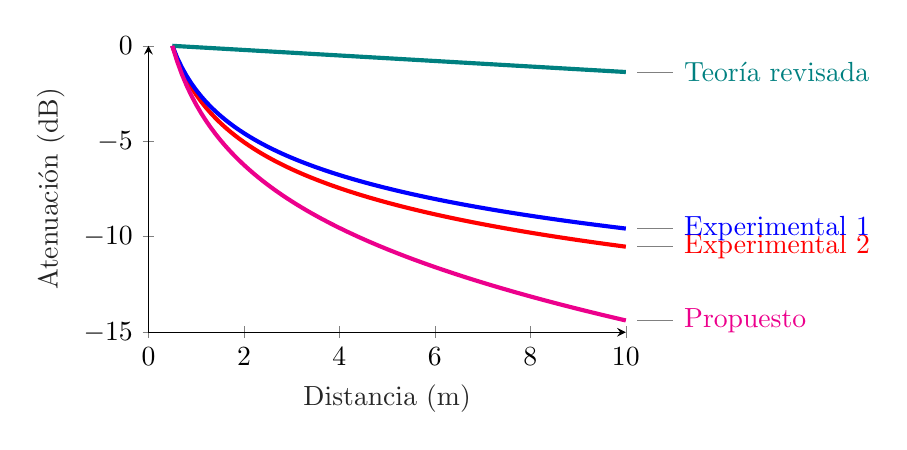
\begin{tikzpicture}

\begin{axis}[%
width=0.5\textwidth,
height=0.3\textwidth,
at={(0\textwidth,0\textwidth)},
scale only axis,
xmin=0,
xmax=10,
xlabel style={font=\color{white!15!black}},
xlabel={Distancia (m)},
ymin=-15,
ymax=0,
clip=false,
axis y line=left,
axis x line=bottom,
ylabel style={font=\color{white!15!black}},
ylabel={Atenuación (dB)},
axis background/.style={fill=white},
legend style={legend cell align=left, align=left, draw=white!15!black}
]
\addplot [color=red, line width=1.5pt]
  table[row sep=crcr]{%
0.5	0\\
0.6	-0.681268180014783\\
0.699999999999999	-1.25295926094489\\
0.800000000000001	-1.74500857405552\\
0.9	-2.1765973186647\\
1	-2.56074716972222\\
1.1	-2.90669889317459\\
1.2	-3.22124454315912\\
1.3	-3.50952085170319\\
1.4	-3.77550565273192\\
1.5	-4.02234137529044\\
1.6	-4.25255314804272\\
1.7	-4.46820017046615\\
1.8	-4.67098342349328\\
1.9	-4.86232399630538\\
2	-5.0434211434293\\
2.1	-5.21529605184143\\
2.2	-5.3788253372246\\
2.3	-5.53476702948237\\
2.4	-5.68378097985607\\
2.5	-5.8264450661754\\
2.6	-5.96326819238567\\
2.7	-6.09470081362625\\
2.8	-6.22114353077266\\
2.9	-6.34295416389409\\
3	-6.46045361629108\\
3.1	-6.57393076878918\\
3.2	-6.68364659036163\\
3.3	-6.78983761082107\\
3.4	-6.89271887067432\\
3.6	-7.08931957790021\\
3.8	-7.27482647442305\\
4	-7.45040225136549\\
4.2	-7.61703696130228\\
4.4	-7.77558049326828\\
4.6	-7.926767766015\\
4.8	-8.07123851294634\\
5	-8.20955299329626\\
5.2	-8.34220459532082\\
5.4	-8.46963004048317\\
5.6	-8.59221771596161\\
5.8	-8.71031453244824\\
6	-8.82423160940138\\
6.2	-8.93424902011984\\
6.4	-9.04061977703894\\
6.6	-9.14357319854545\\
6.9	-9.29204679768539\\
7.2	-9.43392442652032\\
7.5	-9.56975628814219\\
7.8	-9.70002691493798\\
8.1	-9.82516518961904\\
8.4	-9.94555252816818\\
8.7	-10.0615296145471\\
9	-10.1734019839036\\
9.3	-10.2814446824765\\
9.6	-10.3859061813585\\
10	-10.520003668456\\
}node [pos=1,pin=0:Experimental 2] {};

\addplot [color=blue, line width=1.5pt]
  table[row sep=crcr]{%
0.5	0\\
0.6	-0.616533326451801\\
0.699999999999999	-1.13423697060247\\
0.800000000000001	-1.58006665097912\\
0.9	-1.97130424956818\\
1	-2.31968785692216\\
1.1	-2.63355099833748\\
1.2	-2.91902130075722\\
1.3	-3.18073464726344\\
1.4	-3.42228218645896\\
1.5	-3.64650172146513\\
1.6	-3.85567422909482\\
1.7	-4.05166028861399\\
1.8	-4.23599718530805\\
1.9	-4.40996954116169\\
2	-4.57466167952575\\
2.1	-4.7309971094778\\
2.2	-4.87976875057399\\
2.3	-5.02166238498386\\
2.4	-5.1572750784906\\
2.5	-5.28712981115534\\
2.6	-5.41168721572554\\
2.7	-5.53135508318451\\
2.8	-5.64649612597388\\
2.9	-5.75743436821334\\
3	-5.86446044408093\\
3.1	-5.96783602060469\\
3.2	-6.06779751277566\\
3.3	-6.1645592225146\\
3.5	-6.34924554769489\\
3.7	-6.52325926309992\\
3.9	-6.68774631572047\\
4.1	-6.84367844680145\\
4.3	-6.99188671395386\\
4.5	-7.13308733082738\\
4.7	-7.2679018427927\\
4.9	-7.39687306465733\\
5.1	-7.52047780466582\\
5.3	-7.63913712157813\\
5.5	-7.75322466682555\\
5.7	-7.8630735249092\\
5.9	-7.96898186487812\\
6.1	-8.07121764229286\\
6.3	-8.17002253670066\\
6.6	-8.31226984728707\\
6.9	-8.44794078386757\\
7.2	-8.5776062281053\\
7.5	-8.70176622494593\\
7.8	-8.820861206242\\
8.1	-8.93528107943976\\
8.4	-9.04537265034821\\
8.7	-9.15144573311768\\
9	-9.25377821626172\\
9.4	-9.38483170886062\\
9.8	-9.51020492591051\\
10	-9.57090849682801\\
}node [pos=1,pin=0:Experimental 1] {};

\addplot [color=teal, line width=1.5pt]
  table[row sep=crcr]{%
0.5	0\\
10	-1.37246756153321\\
}node [pos=1,pin=0:Teoría revisada] {};

\addplot [color=magenta, line width=1.5pt]
  table[row sep=crcr]{%
0.5	0\\
0.6	-0.80625948743976\\
0.699999999999999	-1.49017441070941\\
0.800000000000001	-2.08454090744978\\
0.9	-2.6105131588871\\
1	-3.08253509145736\\
1.1	-3.51090897000311\\
1.2	-3.90324160586061\\
1.3	-4.26530969541624\\
1.4	-4.60160355609378\\
1.5	-4.9156828168317\\
1.6	-5.21041707979765\\
1.7	-5.48815349398464\\
1.8	-5.75083635819848\\
1.9	-6.00009434365721\\
2	-6.23730531773224\\
2.1	-6.46364533539513\\
2.2	-6.6801262232415\\
2.3	-6.88762480215888\\
2.4	-7.08690588606252\\
2.5	-7.27864058263035\\
2.6	-7.46342100258165\\
2.7	-7.64177219142685\\
2.8	-7.81416189022269\\
2.9	-7.98100858275356\\
3	-8.14268817792413\\
3.1	-8.29953959603374\\
3.2	-8.45186946785358\\
3.3	-8.5999561103969\\
3.4	-8.74405290900408\\
3.6	-9.02118280018142\\
3.8	-9.28488781260367\\
4	-9.53654581364221\\
4.2	-9.77733285826861\\
4.4	-10.0082607730785\\
4.6	-10.2302063789594\\
4.8	-10.4439344898265\\
5	-10.6501162133578\\
5.2	-10.8493436602727\\
5.4	-11.0421418760814\\
5.6	-11.2289786018407\\
5.8	-11.4102723213351\\
6	-11.5863989434692\\
6.2	-11.7576973885423\\
6.4	-11.9244742873256\\
6.6	-12.0870079568325\\
6.8	-12.2455517824032\\
7.1	-12.4763872234221\\
7.4	-12.6994620144316\\
7.7	-12.9153931497372\\
8	-13.1247268488223\\
8.3	-13.3279489835541\\
8.6	-13.5254936531196\\
8.9	-13.7177502880236\\
9.2	-13.9050695759205\\
9.5	-14.087768436244\\
9.8	-14.2661342211709\\
10	-14.382767518173\\
}node [pos=1,pin=0:Propuesto] {};


\end{axis}
\end{tikzpicture}%
    }
    \caption{Comparación de los campos tempranos (1ms-50ms)  del aula OP/S003, EP/0-26M, teórico según \cite{Sato2008} y teórico propuesto por el autor de este trabajo.}
    \label{graf:campostempranos}
\end{figure}
\FloatBarrier



La hipótesis de este comportamiento del campo temprano es que este campo incluye las primeras reflexiones y generalmente, sobretodo en recintos rectangulares, estos \textit{rayos} reflejados tienen la misma dirección de propagación produciendo que la onda acústica esférica del campo directo se comporte en este campo como una onda cilíndrica.

La hipótesis del decaimiento del campo temprano con la inversa de la distancia se basa en los siguientes supuestos:
\begin{description}
\itemsep0em
	\item[Supuesto 1:] El recinto tiene forma rectangular.
	 \item[Supuesto 2:] Sólo existe una fuente sonora y ésta es omnidireccional.
	 \item[Supuesto 3:] El tiempo de integración del campo temprano comprende el intervalo temporal entre 1 ms y 50 ms.
	 \item[Supuesto 4:] El volumen del recinto es superior a 600 $m^3$.
\end{description}

Será objeto de estudio en futuros trabajos el comportamiento del campo temprano en otros recintos con diferentes factores de forma y distintas fuentes para validar esta hipótesis en los diferentes casos o por el contrario confirmar este comportamiento únicamente con los supuestos enunciados anteriormente (el supuesto número 4 ha sido sólo comprobado mediante simulaciones).
\\
\par

Por lo tanto, los cálculos de los campos teniendo en cuenta la propuesta para el campo temprano de incluir la inversa de la distancia, quedan del siguiente modo:
\begin{flalign}
	I_L(r)&= \frac{4W}{A} e^{-\left(\frac{13,82\left(\frac{r}{c}+t_0\right)}{T}\epsilon_L\right)}C_L\\
	I_E (r)&= \frac{4W}{Ar} \left(e^{-\left(\frac{13,82\frac{r}{c}}{T}\epsilon_E\right)}C_E - e^{-\left(\frac{13,82\left(\frac{r}{c}+t_0\right)}{T}\epsilon_L\right)}C_L\right)\label{tempranonuevo}\\
	I_D (r)&= \frac{WQ}{4\pi r^2}C_D\\
	I_{\text{útil}} &= I_D + I_E\\
	I_{\text{perjudicial}} &= I_L
\end{flalign}
\begin{condiciones}[Donde:]
	I_D,I_E,I_L & \rightarrow & Son las intensidades de los campos directo (0-1ms), temprano (1ms-$t$) y tardío ($t$-$\infty$) respectivamente.\\
	\epsilon_L,C_L & \rightarrow & Son los coeficientes del campo perjudicial (Late).\\
	C_D & \rightarrow & Es el coeficiente del campo directo (Direct).\\
	\epsilon_E,C_E & \rightarrow & Son los coeficientes del campo de primeras reflexiones (Early).
\end{condiciones}

Del mismo modo que en la teoría revisada (\ref{teoriarevisada}) se puede calcular directamente el nivel de presión acústica del campo útil (0-$t_0$ ms) y del campo perjudicial ($t_0$ ms- $\infty$).

\begin{flalign}
	L_{p,\text{perjudicial}} (r)&= 10\log_{10} \left[\frac{Z}{p_0^2} \left(\frac{4W}{A} e^{-\left(\frac{13,82\left(\frac{r}{c}+t_0\right)}{T}\epsilon_L\right)}C_L\right)\right]\label{eq:corregida1}\\
	L_{p,\text{útil}} (r)&= 10\log_{10} \left[\frac{Z}{p_0^2} \left(\frac{WQ}{4\pi r^2}C_D + \frac{4W}{Ar} \left(e^{-\left(\frac{13,82\frac{r}{c}}{T}\epsilon_E\right)}C_E - e^{-\left(\frac{13,82\left(\frac{r}{c}+t_0\right)}{T}\epsilon_L\right)}C_L\right)\right)\right]\label{eq:corregida2}
\end{flalign}


Los coeficientes propuestos se obtienen a partir del ajuste de las curvas de la teoría revisada corregida respecto a las curvas obtenidas experimentalmente o con simulaciones acústicas mediante regresión.

\begin{figure}[ht]
    \centering
    {\scalefont{0.8}
    %%%%%%%%%%%%%%%%%%%%%%%%%%%%%%%%%%%%%%%%%%%%%%%%%%%%%%%%%%%%%%%%%%%%%%%%
% Escuela Politécnica Superior de la Universidad de Alicante
% Realizado por: Jose Manuel Requena Plens
% Contacto: info@jmrplens.com / Telegram:@jmrplens
%%%%%%%%%%%%%%%%%%%%%%%%%%%%%%%%%%%%%%%%%%%%%%%%%%%%%%%%%%%%%%%%%%%%%%%%

\definecolor{mycolor1}{rgb}{0.60000,0.00000,0.60000}%
%
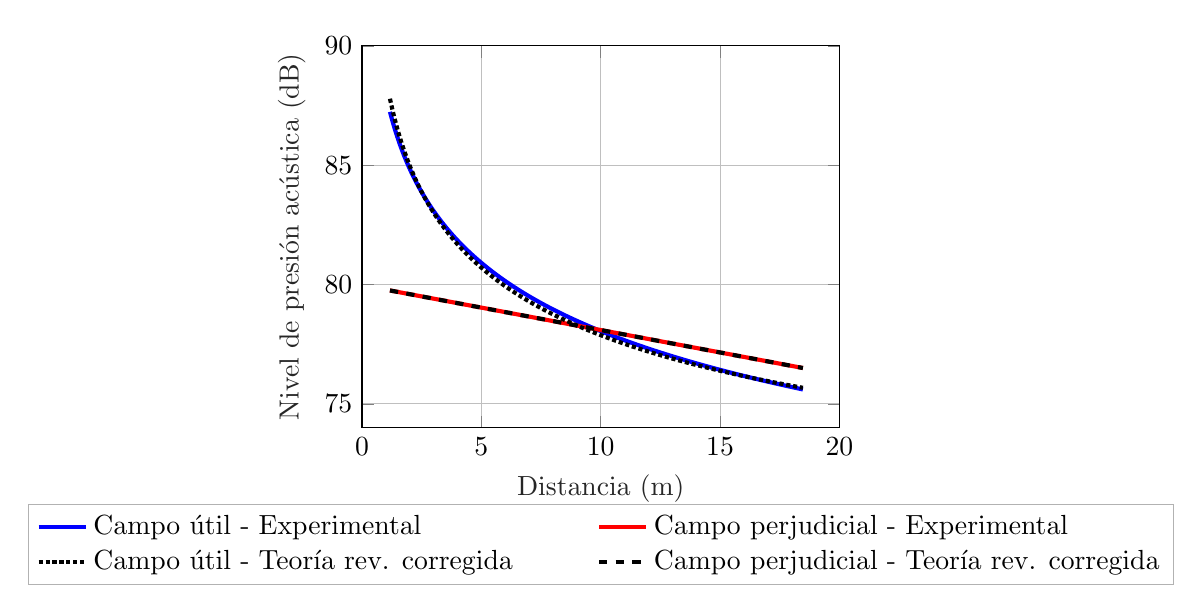
\begin{tikzpicture}

\begin{axis}[%
width=0.5\textwidth,
height=0.4\textwidth,
at={(0\textwidth,0\textwidth)},
scale only axis,
xmin=0,
xmax=20,
xlabel style={font=\color{white!15!black}},
xlabel={Distancia (m)},
ymin=74,
ymax=90,
ylabel style={font=\color{white!15!black}},
ylabel={Nivel de presión acústica (dB)},
axis background/.style={fill=white},
xmajorgrids,
ymajorgrids,
legend style={at={(0.5,-0.03)}, anchor=north, legend cell align=left, align=left, draw=white!15!black},
legend columns = 2,legend style={at={(0.5,-0.2)}, anchor=north, legend cell align=left, align=left, draw=white!70!black, /tikz/every even column/.append style={column sep=1.0cm}}
]

\addplot [color=blue,line width=1.5pt]
  table[row sep=crcr]{%
1.17046999107196	87.2336589559394\\
1.27046999107196	86.8635187039052\\
1.37046999107196	86.5228339435706\\
1.47046999107196	86.2073521092965\\
1.57046999107196	85.9136740685165\\
1.67046999107196	85.6390406951180\\
1.77046999107196	85.3811821373525\\
1.87046999107196	85.1382089255403\\
1.97046999107196	84.9085317287089\\
2.07046999107196	84.6908011761110\\
2.17046999107196	84.4838620157112\\
2.27046999107196	84.2867177015249\\
2.37046999107196	84.0985026897079\\
2.47046999107196	83.9184605159450\\
2.57046999107196	83.7459262660338\\
2.67046999107196	83.5803124251419\\
2.77046999107196	83.4210973542065\\
2.87046999107196	83.2678158298440\\
2.97046999107196	83.1200512202337\\
3.07046999107196	82.9774289692446\\
3.17046999107196	82.8396111351343\\
3.27046999107196	82.7062917856878\\
3.37046999107196	82.5771930937365\\
3.47046999107196	82.4520620091675\\
3.57046999107196	82.3306674083460\\
3.67046999107196	82.2127976411683\\
3.77046999107196	82.0982584110805\\
3.87046999107196	81.9868709353349\\
3.97046999107196	81.8784703422348\\
4.07046999107196	81.7729042697051\\
4.17046999107196	81.6700316356279\\
4.27046999107196	81.5697215553191\\
4.37046999107196	81.4718523855414\\
4.47046999107196	81.3763108777358\\
4.57046999107196	81.2829914258524\\
4.67046999107196	81.1917953963946\\
4.77046999107196	81.1026305301391\\
4.87046999107196	81.0154104065358\\
4.97046999107196	80.9300539630801\\
5.07046999107196	80.8464850630338\\
5.17046999107196	80.7646321057808\\
5.27046999107196	80.6844276748772\\
5.37046999107196	80.6058082195097\\
5.47046999107196	80.5287137656321\\
5.57046999107196	80.4530876535285\\
5.67046999107196	80.3788762989580\\
5.77046999107196	80.3060289753870\\
5.87046999107196	80.2344976151168\\
5.97046999107196	80.1642366273757\\
6.07046999107196	80.0952027316711\\
6.17046999107196	80.0273548048921\\
6.27046999107196	79.9606537408272\\
6.37046999107196	79.8950623209056\\
6.47046999107196	79.8305450951077\\
6.57046999107196	79.7670682720990\\
6.67046999107196	79.7045996177450\\
6.77046999107196	79.6431083612535\\
6.87046999107196	79.5825651082663\\
6.97046999107196	79.5229417602936\\
7.07046999107196	79.4642114399443\\
7.17046999107196	79.4063484214599\\
7.27046999107196	79.3493280661069\\
7.37046999107196	79.2931267620270\\
7.47046999107196	79.2377218681808\\
7.57046999107196	79.1830916620572\\
7.67046999107196	79.1292152908466\\
7.77046999107196	79.0760727258101\\
7.87046999107196	79.0236447195947\\
7.97046999107196	78.9719127662702\\
8.07046999107196	78.9208590638830\\
8.17046999107196	78.8704664793393\\
8.27046999107196	78.8207185154449\\
8.37046999107196	78.7715992799464\\
8.47046999107196	78.7230934564292\\
8.57046999107196	78.6751862769409\\
8.67046999107196	78.6278634962176\\
8.77046999107196	78.5811113674045\\
8.87046999107196	78.5349166191655\\
8.97046999107196	78.4892664340892\\
9.07046999107196	78.4441484283047\\
9.17046999107196	78.3995506322248\\
9.27046999107196	78.3554614723455\\
9.37046999107196	78.3118697540309\\
9.47046999107196	78.2687646452214\\
9.57046999107196	78.2261356610059\\
9.67046999107196	78.1839726490046\\
9.77046999107196	78.1422657755106\\
9.87046999107196	78.1010055123445\\
9.97046999107196	78.0601826243787\\
10.0704699910720	78.0197881576899\\
10.1704699910720	77.9798134283032\\
10.2704699910720	77.9402500114924\\
10.3704699910720	77.9010897316038\\
10.4704699910720	77.8623246523738\\
10.5704699910720	77.8239470677103\\
10.6704699910720	77.7859494929139\\
10.7704699910720	77.7483246563112\\
10.8704699910720	77.7110654912799\\
10.9704699910720	77.6741651286421\\
11.0704699910720	77.6376168894063\\
11.1704699910720	77.6014142778394\\
11.2704699910720	77.5655509748499\\
11.3704699910720	77.5300208316670\\
11.4704699910720	77.4948178637990\\
11.5704699910720	77.4599362452564\\
11.6704699910720	77.4253703030263\\
11.7704699910720	77.3911145117850\\
11.8704699910720	77.3571634888362\\
11.9704699910720	77.3235119892643\\
12.0704699910720	77.2901549012903\\
12.1704699910720	77.2570872418225\\
12.2704699910720	77.2243041521902\\
12.3704699910720	77.1918008940526\\
12.4704699910720	77.1595728454739\\
12.5704699910720	77.1276154971575\\
12.6704699910720	77.0959244488293\\
12.7704699910720	77.0644954057668\\
12.8704699910720	77.0333241754626\\
12.9704699910720	77.0024066644204\\
13.0704699910720	76.9717388750740\\
13.1704699910720	76.9413169028254\\
13.2704699910720	76.9111369331956\\
13.3704699910720	76.8811952390844\\
13.4704699910720	76.8514881781324\\
13.5704699910720	76.8220121901820\\
13.6704699910720	76.7927637948322\\
13.7704699910720	76.7637395890838\\
13.8704699910720	76.7349362450709\\
13.9704699910720	76.7063505078736\\
14.0704699910720	76.6779791934109\\
14.1704699910720	76.6498191864079\\
14.2704699910720	76.6218674384358\\
14.3704699910720	76.5941209660208\\
14.4704699910720	76.5665768488192\\
14.5704699910720	76.5392322278563\\
14.6704699910720	76.5120843038256\\
14.7704699910720	76.4851303354469\\
14.8704699910720	76.4583676378801\\
14.9704699910720	76.4317935811927\\
15.0704699910720	76.4054055888786\\
15.1704699910720	76.3792011364272\\
15.2704699910720	76.3531777499390\\
15.3704699910720	76.3273330047873\\
15.4704699910720	76.3016645243238\\
15.5704699910720	76.2761699786264\\
15.6704699910720	76.2508470832871\\
15.7704699910720	76.2256935982390\\
15.8704699910720	76.2007073266210\\
15.9704699910720	76.1758861136784\\
16.0704699910720	76.1512278456979\\
16.1704699910720	76.1267304489765\\
16.2704699910720	76.1023918888216\\
16.3704699910720	76.0782101685833\\
16.4704699910720	76.0541833287155\\
16.5704699910720	76.0303094458659\\
16.6704699910720	76.0065866319939\\
16.7704699910720	75.9830130335151\\
16.8704699910720	75.9595868304712\\
16.9704699910720	75.9363062357251\\
17.0704699910720	75.9131694941793\\
17.1704699910720	75.8901748820183\\
17.2704699910720	75.8673207059721\\
17.3704699910720	75.8446053026022\\
17.4704699910720	75.8220270376074\\
17.5704699910720	75.7995843051504\\
17.6704699910720	75.7772755272031\\
17.7704699910720	75.7550991529110\\
17.8704699910720	75.7330536579753\\
17.9704699910720	75.7111375440527\\
18.0704699910720	75.6893493381717\\
18.1704699910720	75.6676875921654\\
18.2704699910720	75.6461508821200\\
18.3704699910720	75.6247378078386\\
18.4704699910720	75.6034469923192\\
};
\addlegendentry{Campo útil - Experimental}

\addplot [color=red,line width=1.5pt]
  table[row sep=crcr]{%
1.17046999107196	79.7499907626293\\
1.27046999107196	79.7312109696139\\
1.37046999107196	79.7124311765986\\
1.47046999107196	79.6936513835832\\
1.57046999107196	79.6748715905678\\
1.67046999107196	79.6560917975524\\
1.77046999107196	79.6373120045370\\
1.87046999107196	79.6185322115217\\
1.97046999107196	79.5997524185063\\
2.07046999107196	79.5809726254909\\
2.17046999107196	79.5621928324755\\
2.27046999107196	79.5434130394602\\
2.37046999107196	79.5246332464448\\
2.47046999107196	79.5058534534294\\
2.57046999107196	79.4870736604140\\
2.67046999107196	79.4682938673986\\
2.77046999107196	79.4495140743833\\
2.87046999107196	79.4307342813679\\
2.97046999107196	79.4119544883525\\
3.07046999107196	79.3931746953371\\
3.17046999107196	79.3743949023218\\
3.27046999107196	79.3556151093064\\
3.37046999107196	79.3368353162910\\
3.47046999107196	79.3180555232756\\
3.57046999107196	79.2992757302602\\
3.67046999107196	79.2804959372449\\
3.77046999107196	79.2617161442295\\
3.87046999107196	79.2429363512141\\
3.97046999107196	79.2241565581987\\
4.07046999107196	79.2053767651834\\
4.17046999107196	79.1865969721680\\
4.27046999107196	79.1678171791526\\
4.37046999107196	79.1490373861372\\
4.47046999107196	79.1302575931218\\
4.57046999107196	79.1114778001065\\
4.67046999107196	79.0926980070911\\
4.77046999107196	79.0739182140757\\
4.87046999107196	79.0551384210603\\
4.97046999107196	79.0363586280450\\
5.07046999107196	79.0175788350296\\
5.17046999107196	78.9987990420142\\
5.27046999107196	78.9800192489988\\
5.37046999107196	78.9612394559834\\
5.47046999107196	78.9424596629681\\
5.57046999107196	78.9236798699527\\
5.67046999107196	78.9049000769373\\
5.77046999107196	78.8861202839219\\
5.87046999107196	78.8673404909065\\
5.97046999107196	78.8485606978912\\
6.07046999107196	78.8297809048758\\
6.17046999107196	78.8110011118604\\
6.27046999107196	78.7922213188450\\
6.37046999107196	78.7734415258297\\
6.47046999107196	78.7546617328143\\
6.57046999107196	78.7358819397989\\
6.67046999107196	78.7171021467835\\
6.77046999107196	78.6983223537682\\
6.87046999107196	78.6795425607528\\
6.97046999107196	78.6607627677374\\
7.07046999107196	78.6419829747220\\
7.17046999107196	78.6232031817066\\
7.27046999107196	78.6044233886913\\
7.37046999107196	78.5856435956759\\
7.47046999107196	78.5668638026605\\
7.57046999107196	78.5480840096451\\
7.67046999107196	78.5293042166297\\
7.77046999107196	78.5105244236144\\
7.87046999107196	78.4917446305990\\
7.97046999107196	78.4729648375836\\
8.07046999107196	78.4541850445682\\
8.17046999107196	78.4354052515529\\
8.27046999107196	78.4166254585375\\
8.37046999107196	78.3978456655221\\
8.47046999107196	78.3790658725067\\
8.57046999107196	78.3602860794913\\
8.67046999107196	78.3415062864760\\
8.77046999107196	78.3227264934606\\
8.87046999107196	78.3039467004452\\
8.97046999107196	78.2851669074298\\
9.07046999107196	78.2663871144144\\
9.17046999107196	78.2476073213991\\
9.27046999107196	78.2288275283837\\
9.37046999107196	78.2100477353683\\
9.47046999107196	78.1912679423529\\
9.57046999107196	78.1724881493376\\
9.67046999107196	78.1537083563222\\
9.77046999107196	78.1349285633068\\
9.87046999107196	78.1161487702914\\
9.97046999107196	78.0973689772761\\
10.0704699910720	78.0785891842607\\
10.1704699910720	78.0598093912453\\
10.2704699910720	78.0410295982299\\
10.3704699910720	78.0222498052145\\
10.4704699910720	78.0034700121992\\
10.5704699910720	77.9846902191838\\
10.6704699910720	77.9659104261684\\
10.7704699910720	77.9471306331530\\
10.8704699910720	77.9283508401376\\
10.9704699910720	77.9095710471223\\
11.0704699910720	77.8907912541069\\
11.1704699910720	77.8720114610915\\
11.2704699910720	77.8532316680761\\
11.3704699910720	77.8344518750608\\
11.4704699910720	77.8156720820454\\
11.5704699910720	77.7968922890300\\
11.6704699910720	77.7781124960146\\
11.7704699910720	77.7593327029993\\
11.8704699910720	77.7405529099839\\
11.9704699910720	77.7217731169685\\
12.0704699910720	77.7029933239531\\
12.1704699910720	77.6842135309377\\
12.2704699910720	77.6654337379224\\
12.3704699910720	77.6466539449070\\
12.4704699910720	77.6278741518916\\
12.5704699910720	77.6090943588762\\
12.6704699910720	77.5903145658608\\
12.7704699910720	77.5715347728455\\
12.8704699910720	77.5527549798301\\
12.9704699910720	77.5339751868147\\
13.0704699910720	77.5151953937993\\
13.1704699910720	77.4964156007840\\
13.2704699910720	77.4776358077686\\
13.3704699910720	77.4588560147532\\
13.4704699910720	77.4400762217378\\
13.5704699910720	77.4212964287224\\
13.6704699910720	77.4025166357071\\
13.7704699910720	77.3837368426917\\
13.8704699910720	77.3649570496763\\
13.9704699910720	77.3461772566609\\
14.0704699910720	77.3273974636456\\
14.1704699910720	77.3086176706302\\
14.2704699910720	77.2898378776148\\
14.3704699910720	77.2710580845994\\
14.4704699910720	77.2522782915840\\
14.5704699910720	77.2334984985687\\
14.6704699910720	77.2147187055533\\
14.7704699910720	77.1959389125379\\
14.8704699910720	77.1771591195225\\
14.9704699910720	77.1583793265071\\
15.0704699910720	77.1395995334918\\
15.1704699910720	77.1208197404764\\
15.2704699910720	77.1020399474610\\
15.3704699910720	77.0832601544456\\
15.4704699910720	77.0644803614303\\
15.5704699910720	77.0457005684149\\
15.6704699910720	77.0269207753995\\
15.7704699910720	77.0081409823841\\
15.8704699910720	76.9893611893687\\
15.9704699910720	76.9705813963534\\
16.0704699910720	76.9518016033380\\
16.1704699910720	76.9330218103226\\
16.2704699910720	76.9142420173072\\
16.3704699910720	76.8954622242919\\
16.4704699910720	76.8766824312765\\
16.5704699910720	76.8579026382611\\
16.6704699910720	76.8391228452457\\
16.7704699910720	76.8203430522303\\
16.8704699910720	76.8015632592150\\
16.9704699910720	76.7827834661996\\
17.0704699910720	76.7640036731842\\
17.1704699910720	76.7452238801688\\
17.2704699910720	76.7264440871535\\
17.3704699910720	76.7076642941381\\
17.4704699910720	76.6888845011227\\
17.5704699910720	76.6701047081073\\
17.6704699910720	76.6513249150919\\
17.7704699910720	76.6325451220766\\
17.8704699910720	76.6137653290612\\
17.9704699910720	76.5949855360458\\
18.0704699910720	76.5762057430304\\
18.1704699910720	76.5574259500150\\
18.2704699910720	76.5386461569997\\
18.3704699910720	76.5198663639843\\
18.4704699910720	76.5010865709689\\
};
\addlegendentry{Campo perjudicial - Experimental}

\addplot [color=black, densely dotted, line width=1.5pt]
  table[row sep=crcr]{%
1.17046999107196	87.7832978395894\\
1.27046999107196	87.3355562101656\\
1.37046999107196	86.9275760618408\\
1.47046999107196	86.5532412580561\\
1.57046999107196	86.2077154587765\\
1.67046999107196	85.8871129217553\\
1.77046999107196	85.5882678912612\\
1.87046999107196	85.3085693390714\\
1.97046999107196	85.0458401500994\\
2.07046999107196	84.7982472233551\\
2.17046999107196	84.5642335124690\\
2.27046999107196	84.3424659174261\\
2.37046999107196	84.1317948148505\\
2.47046999107196	83.9312222593389\\
2.57046999107196	83.7398767312620\\
2.67046999107196	83.5569928872912\\
2.77046999107196	83.3818951766857\\
2.87046999107196	83.2139844755053\\
2.97046999107196	83.0527270992434\\
3.07046999107196	82.8976457063823\\
3.17046999107196	82.7483117175832\\
3.27046999107196	82.6043389589594\\
3.37046999107196	82.4653783009903\\
3.47046999107196	82.3311131126615\\
3.57046999107196	82.2012553872697\\
3.67046999107196	82.0755424248648\\
3.77046999107196	81.9537339785441\\
3.87046999107196	81.8356097892994\\
3.97046999107196	81.7209674479386\\
4.07046999107196	81.6096205336204\\
4.17046999107196	81.5013969873527\\
4.27046999107196	81.3961376859184\\
4.37046999107196	81.2936951874462\\
4.47046999107196	81.1939326245364\\
4.57046999107196	81.0967227246913\\
4.67046999107196	81.0019469409548\\
4.77046999107196	80.9094946782786\\
4.87046999107196	80.8192626032951\\
4.97046999107196	80.7311540269805\\
5.07046999107196	80.6450783512045\\
5.17046999107196	80.5609505714254\\
5.27046999107196	80.4786908288619\\
5.37046999107196	80.3982240063737\\
5.47046999107196	80.3194793630501\\
5.57046999107196	80.2423902031607\\
5.67046999107196	80.1668935756745\\
5.77046999107196	80.0929300010386\\
5.87046999107196	80.0204432223097\\
5.97046999107196	79.9493799780912\\
6.07046999107196	79.8796897950305\\
6.17046999107196	79.8113247978966\\
6.27046999107196	79.7442395354854\\
6.37046999107196	79.6783908208040\\
6.47046999107196	79.6137375841535\\
6.57046999107196	79.5502407378870\\
6.67046999107196	79.4878630517501\\
6.77046999107196	79.4265690378289\\
6.87046999107196	79.3663248442328\\
6.97046999107196	79.3070981567322\\
7.07046999107196	79.2488581076482\\
7.17046999107196	79.1915751913652\\
7.27046999107196	79.1352211858972\\
7.37046999107196	79.0797690799992\\
7.47046999107196	79.0251930053571\\
7.57046999107196	78.9714681734429\\
7.67046999107196	78.9185708166530\\
7.77046999107196	78.8664781333887\\
7.87046999107196	78.8151682367662\\
7.97046999107196	78.7646201066735\\
8.07046999107196	78.7148135449156\\
8.17046999107196	78.6657291332135\\
8.27046999107196	78.6173481938418\\
8.37046999107196	78.5696527527100\\
8.47046999107196	78.5226255047074\\
8.57046999107196	78.4762497811472\\
8.67046999107196	78.4305095191612\\
8.77046999107196	78.3853892329042\\
8.87046999107196	78.3408739864438\\
8.97046999107196	78.2969493682182\\
9.07046999107196	78.2536014669540\\
9.17046999107196	78.2108168489460\\
9.27046999107196	78.1685825366080\\
9.37046999107196	78.1268859882097\\
9.47046999107196	78.0857150787222\\
9.57046999107196	78.0450580817012\\
9.67046999107196	78.0049036521398\\
9.77046999107196	77.9652408102310\\
9.87046999107196	77.9260589259814\\
9.97046999107196	77.8873477046243\\
10.0704699910720	77.8490971727820\\
10.1704699910720	77.8112976653328\\
10.2704699910720	77.7739398129392\\
10.3704699910720	77.7370145301982\\
10.4704699910720	77.7005130043771\\
10.5704699910720	77.6644266847006\\
10.6704699910720	77.6287472721564\\
10.7704699910720	77.5934667097902\\
10.8704699910720	77.5585771734630\\
10.9704699910720	77.5240710630422\\
11.0704699910720	77.4899409940054\\
11.1704699910720	77.4561797894313\\
11.2704699910720	77.4227804723582\\
11.3704699910720	77.3897362584898\\
11.4704699910720	77.3570405492283\\
11.5704699910720	77.3246869250198\\
11.6704699910720	77.2926691389926\\
11.7704699910720	77.2609811108755\\
11.8704699910720	77.2296169211798\\
11.9704699910720	77.1985708056326\\
12.0704699910720	77.1678371498474\\
12.1704699910720	77.1374104842211\\
12.2704699910720	77.1072854790451\\
12.3704699910720	77.0774569398207\\
12.4704699910720	77.0479198027671\\
12.5704699910720	77.0186691305150\\
12.6704699910720	76.9897001079745\\
12.7704699910720	76.9610080383698\\
12.8704699910720	76.9325883394330\\
12.9704699910720	76.9044365397488\\
13.0704699910720	76.8765482752434\\
13.1704699910720	76.8489192858109\\
13.2704699910720	76.8215454120701\\
13.3704699910720	76.7944225922469\\
13.4704699910720	76.7675468591751\\
13.5704699910720	76.7409143374121\\
13.6704699910720	76.7145212404618\\
13.7704699910720	76.6883638681024\\
13.8704699910720	76.6624386038132\\
13.9704699910720	76.6367419122955\\
14.0704699910720	76.6112703370851\\
14.1704699910720	76.5860204982509\\
14.2704699910720	76.5609890901764\\
14.3704699910720	76.5361728794212\\
14.4704699910720	76.5115687026580\\
14.5704699910720	76.4871734646825\\
14.6704699910720	76.4629841364932\\
14.7704699910720	76.4389977534380\\
14.8704699910720	76.4152114134249\\
14.9704699910720	76.3916222751940\\
15.0704699910720	76.3682275566489\\
15.1704699910720	76.3450245332437\\
15.2704699910720	76.3220105364257\\
15.3704699910720	76.2991829521287\\
15.4704699910720	76.2765392193174\\
15.5704699910720	76.2540768285793\\
15.6704699910720	76.2317933207631\\
15.7704699910720	76.2096862856612\\
15.8704699910720	76.1877533607349\\
15.9704699910720	76.1659922298809\\
16.0704699910720	76.1444006222367\\
16.1704699910720	76.1229763110245\\
16.2704699910720	76.1017171124312\\
16.3704699910720	76.0806208845234\\
16.4704699910720	76.0596855261972\\
16.5704699910720	76.0389089761591\\
16.6704699910720	76.0182892119395\\
16.7704699910720	75.9978242489358\\
16.8704699910720	75.9775121394849\\
16.9704699910720	75.9573509719631\\
17.0704699910720	75.9373388699144\\
17.1704699910720	75.9174739912034\\
17.2704699910720	75.8977545271942\\
17.3704699910720	75.8781787019538\\
17.4704699910720	75.8587447714776\\
17.5704699910720	75.8394510229395\\
17.6704699910720	75.8202957739617\\
17.7704699910720	75.8012773719074\\
17.8704699910720	75.7823941931924\\
17.9704699910720	75.7636446426172\\
18.0704699910720	75.7450271527179\\
18.1704699910720	75.7265401831352\\
18.2704699910720	75.7081822200012\\
18.3704699910720	75.6899517753437\\
18.4704699910720	75.6718473865063\\
};
\addlegendentry{Campo útil - Teoría rev. corregida}

\addplot [color=black, dashed, line width=1.5pt]
  table[row sep=crcr]{%
1.17046999107196	79.7499907626304\\
1.27046999107196	79.7312109696150\\
1.37046999107196	79.7124311765997\\
1.47046999107196	79.6936513835843\\
1.57046999107196	79.6748715905689\\
1.67046999107196	79.6560917975536\\
1.77046999107196	79.6373120045382\\
1.87046999107196	79.6185322115228\\
1.97046999107196	79.5997524185075\\
2.07046999107196	79.5809726254921\\
2.17046999107196	79.5621928324767\\
2.27046999107196	79.5434130394614\\
2.37046999107196	79.5246332464460\\
2.47046999107196	79.5058534534306\\
2.57046999107196	79.4870736604153\\
2.67046999107196	79.4682938673999\\
2.77046999107196	79.4495140743845\\
2.87046999107196	79.4307342813692\\
2.97046999107196	79.4119544883538\\
3.07046999107196	79.3931746953384\\
3.17046999107196	79.3743949023231\\
3.27046999107196	79.3556151093077\\
3.37046999107196	79.3368353162923\\
3.47046999107196	79.3180555232770\\
3.57046999107196	79.2992757302616\\
3.67046999107196	79.2804959372462\\
3.77046999107196	79.2617161442309\\
3.87046999107196	79.2429363512155\\
3.97046999107196	79.2241565582002\\
4.07046999107196	79.2053767651848\\
4.17046999107196	79.1865969721694\\
4.27046999107196	79.1678171791540\\
4.37046999107196	79.1490373861387\\
4.47046999107196	79.1302575931233\\
4.57046999107196	79.1114778001080\\
4.67046999107196	79.0926980070926\\
4.77046999107196	79.0739182140772\\
4.87046999107196	79.0551384210619\\
4.97046999107196	79.0363586280465\\
5.07046999107196	79.0175788350311\\
5.17046999107196	78.9987990420158\\
5.27046999107196	78.9800192490004\\
5.37046999107196	78.9612394559850\\
5.47046999107196	78.9424596629697\\
5.57046999107196	78.9236798699543\\
5.67046999107196	78.9049000769389\\
5.77046999107196	78.8861202839236\\
5.87046999107196	78.8673404909082\\
5.97046999107196	78.8485606978928\\
6.07046999107196	78.8297809048775\\
6.17046999107196	78.8110011118621\\
6.27046999107196	78.7922213188467\\
6.37046999107196	78.7734415258314\\
6.47046999107196	78.7546617328160\\
6.57046999107196	78.7358819398006\\
6.67046999107196	78.7171021467853\\
6.77046999107196	78.6983223537699\\
6.87046999107196	78.6795425607545\\
6.97046999107196	78.6607627677392\\
7.07046999107196	78.6419829747238\\
7.17046999107196	78.6232031817084\\
7.27046999107196	78.6044233886931\\
7.37046999107196	78.5856435956777\\
7.47046999107196	78.5668638026623\\
7.57046999107196	78.5480840096470\\
7.67046999107196	78.5293042166316\\
7.77046999107196	78.5105244236162\\
7.87046999107196	78.4917446306009\\
7.97046999107196	78.4729648375855\\
8.07046999107196	78.4541850445701\\
8.17046999107196	78.4354052515548\\
8.27046999107196	78.4166254585394\\
8.37046999107196	78.3978456655240\\
8.47046999107196	78.3790658725087\\
8.57046999107196	78.3602860794933\\
8.67046999107196	78.3415062864779\\
8.77046999107196	78.3227264934626\\
8.87046999107196	78.3039467004472\\
8.97046999107196	78.2851669074318\\
9.07046999107196	78.2663871144165\\
9.17046999107196	78.2476073214011\\
9.27046999107196	78.2288275283857\\
9.37046999107196	78.2100477353704\\
9.47046999107196	78.1912679423550\\
9.57046999107196	78.1724881493396\\
9.67046999107196	78.1537083563243\\
9.77046999107196	78.1349285633089\\
9.87046999107196	78.1161487702936\\
9.97046999107196	78.0973689772782\\
10.0704699910720	78.0785891842628\\
10.1704699910720	78.0598093912474\\
10.2704699910720	78.0410295982321\\
10.3704699910720	78.0222498052167\\
10.4704699910720	78.0034700122014\\
10.5704699910720	77.9846902191860\\
10.6704699910720	77.9659104261706\\
10.7704699910720	77.9471306331553\\
10.8704699910720	77.9283508401399\\
10.9704699910720	77.9095710471245\\
11.0704699910720	77.8907912541092\\
11.1704699910720	77.8720114610938\\
11.2704699910720	77.8532316680784\\
11.3704699910720	77.8344518750631\\
11.4704699910720	77.8156720820477\\
11.5704699910720	77.7968922890323\\
11.6704699910720	77.7781124960170\\
11.7704699910720	77.7593327030016\\
11.8704699910720	77.7405529099862\\
11.9704699910720	77.7217731169709\\
12.0704699910720	77.7029933239555\\
12.1704699910720	77.6842135309401\\
12.2704699910720	77.6654337379248\\
12.3704699910720	77.6466539449094\\
12.4704699910720	77.6278741518940\\
12.5704699910720	77.6090943588787\\
12.6704699910720	77.5903145658633\\
12.7704699910720	77.5715347728479\\
12.8704699910720	77.5527549798326\\
12.9704699910720	77.5339751868172\\
13.0704699910720	77.5151953938018\\
13.1704699910720	77.4964156007865\\
13.2704699910720	77.4776358077711\\
13.3704699910720	77.4588560147557\\
13.4704699910720	77.4400762217404\\
13.5704699910720	77.4212964287250\\
13.6704699910720	77.4025166357096\\
13.7704699910720	77.3837368426943\\
13.8704699910720	77.3649570496789\\
13.9704699910720	77.3461772566635\\
14.0704699910720	77.3273974636482\\
14.1704699910720	77.3086176706328\\
14.2704699910720	77.2898378776174\\
14.3704699910720	77.2710580846021\\
14.4704699910720	77.2522782915867\\
14.5704699910720	77.2334984985713\\
14.6704699910720	77.2147187055560\\
14.7704699910720	77.1959389125406\\
14.8704699910720	77.1771591195252\\
14.9704699910720	77.1583793265099\\
15.0704699910720	77.1395995334945\\
15.1704699910720	77.1208197404791\\
15.2704699910720	77.1020399474638\\
15.3704699910720	77.0832601544484\\
15.4704699910720	77.0644803614330\\
15.5704699910720	77.0457005684177\\
15.6704699910720	77.0269207754023\\
15.7704699910720	77.0081409823869\\
15.8704699910720	76.9893611893716\\
15.9704699910720	76.9705813963562\\
16.0704699910720	76.9518016033408\\
16.1704699910720	76.9330218103255\\
16.2704699910720	76.9142420173101\\
16.3704699910720	76.8954622242947\\
16.4704699910720	76.8766824312794\\
16.5704699910720	76.8579026382640\\
16.6704699910720	76.8391228452486\\
16.7704699910720	76.8203430522333\\
16.8704699910720	76.8015632592179\\
16.9704699910720	76.7827834662026\\
17.0704699910720	76.7640036731872\\
17.1704699910720	76.7452238801718\\
17.2704699910720	76.7264440871564\\
17.3704699910720	76.7076642941411\\
17.4704699910720	76.6888845011257\\
17.5704699910720	76.6701047081103\\
17.6704699910720	76.6513249150950\\
17.7704699910720	76.6325451220796\\
17.8704699910720	76.6137653290643\\
17.9704699910720	76.5949855360489\\
18.0704699910720	76.5762057430335\\
18.1704699910720	76.5574259500181\\
18.2704699910720	76.5386461570028\\
18.3704699910720	76.5198663639874\\
18.4704699910720	76.5010865709721\\
};
\addlegendentry{Campo perjudicial - Teoría rev. corregida}



\end{axis}
\end{tikzpicture}%
    }
    \caption{Comparación de los campos acústicos obtenidos experimentalmente y mediante la teoría revisada corregida. El tiempo de integración es 50 ms y los coeficientes: $\epsilon_L=1.244$, $C_L=1.268$, $C_D=1.070$, $\epsilon_E=-0.296$ y $C_E=3.588$.}
    \label{graf:corregida}
\end{figure}
\FloatBarrier

\section{Otros conceptos}
En este trabajo se han utilizado en las medidas in situ señales MLS, y tanto en las medidas in situ como en los modelos se han obtenido las respuestas al impulso en distintas ubicaciones del recinto (receptores), a continuación se describen estos conceptos.


\subsection{Señal MLS}

Una señal MLS (\textit{maximum length sequence}) está constituída por variaciones pseudoaleatorias entre -1 y 1, con periodo $P=\nicefrac{2^N-1}{f_{clock}}$ ($N$ es el número de bits y $f_{clock}$ es la frecuencia de reloj del sistema que genera la señal MLS) y una respuesta en frecuencia plana, es decir, igual al ruido blanco (apartado \ref{ruidos}). La pseudoaleatoridad de la señal se refiere a que es periódica y en cada periodo tiene una aleatoriedad conocida, esto permite comparar correctamente la señal emitida con la captada.

\begin{figure}[ht]
    \centering
    {\scalefont{0.8}
    %%%%%%%%%%%%%%%%%%%%%%%%%%%%%%%%%%%%%%%%%%%%%%%%%%%%%%%%%%%%%%%%%%%%%%%%
% Escuela Politécnica Superior de la Universidad de Alicante
% Realizado por: Jose Manuel Requena Plens
% Contacto: info@jmrplens.com / Telegram:@jmrplens
%%%%%%%%%%%%%%%%%%%%%%%%%%%%%%%%%%%%%%%%%%%%%%%%%%%%%%%%%%%%%%%%%%%%%%%%

\definecolor{mycolor1}{rgb}{0.00000,0.44700,0.74100}%
%

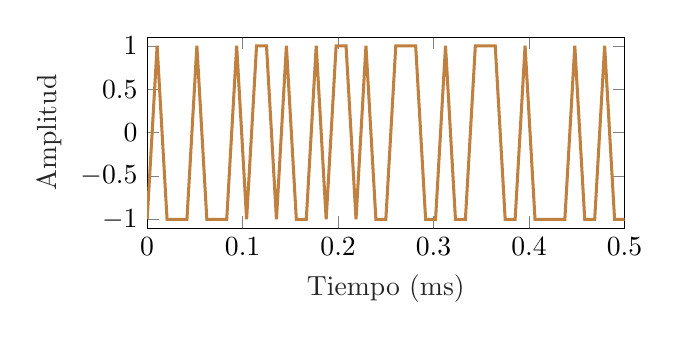
\begin{tikzpicture}

\begin{axis}[%
width=0.5\textwidth,
height=0.2\textwidth,
at={(0\textwidth,0\textwidth)},
scale only axis,
xmin=0,
xmax=0.5,
xlabel style={font=\color{white!15!black}},
xlabel={Tiempo (ms)},
ymin=-1.1,
ymax=1.1,
ylabel style={font=\color{white!15!black}},
ylabel={Amplitud},
axis background/.style={fill=white},
legend style={legend cell align=left, align=left, draw=white!15!black}
]
\addplot [color=brown, line width=1.1]
  table[row sep=crcr]{%
0	-1.00003051875\\
0.0104166666666667	1\\
0.0208333333333333	-1.00003051875\\
0.0416666666666667	-1.00003051875\\
0.0520833333333335	1\\
0.0625	-1.00003051875\\
0.0833333333333335	-1.00003051875\\
0.0937500000000002	1\\
0.104166666666667	-1.00003051875\\
0.114583333333333	1\\
0.125	1\\
0.135416666666667	-1.00003051875\\
0.145833333333333	1\\
0.15625	-1.00003051875\\
0.166666666666667	-1.00003051875\\
0.177083333333333	1\\
0.1875	-1.00003051875\\
0.197916666666667	1\\
0.208333333333333	1\\
0.21875	-1.00003051875\\
0.229166666666667	1\\
0.239583333333333	-1.00003051875\\
0.25	-1.00003051875\\
0.260416666666667	1\\
0.28125	1\\
0.291666666666667	-1.00003051875\\
0.302083333333333	-1.00003051875\\
0.3125	1\\
0.322916666666667	-1.00003051875\\
0.333333333333333	-1.00003051875\\
0.34375	1\\
0.364583333333333	1\\
0.375	-1.00003051875\\
0.385416666666667	-1.00003051875\\
0.395833333333333	1\\
0.40625	-1.00003051875\\
0.4375	-1.00003051875\\
0.447916666666667	1\\
0.458333333333333	-1.00003051875\\
0.46875	-1.00003051875\\
0.479166666666667	1\\
0.489583333333333	-1.00003051875\\
0.520833333333333	-1.00003051875\\
};


\end{axis}
\end{tikzpicture}%
    }
    \caption{Fracción temporal de una señal MLS.}
    \label{graf:mls}
\end{figure}


Esta señal permite mediante un proceso, que se resume a continuación, eliminar ruidos de fondo y obtener una respuesta en frecuencia y temporal de la probeta de medida (material, recinto, equipo, etc) definida.

La señal se basa en la teoría de secuencias de registro de desplazamiento ampliamente desarrollada en \cite{Golomb1967}. Una vez emitida y captada la señal en los puntos deseados, se puede obtener la respuesta al impulso (apartado \ref{respimpulso}) mediante una correlación cruzada de la señal emitida y la captada o mediante la transformada de Hadamard \citep{Sylvester1908}. 

El desarrollo extenso de estos procesos se pueden consultar en \cite{Cohn1977} o \cite{Sarwate1980}. En este trabajo no se va a extender la descripción de la MLS ni su proceso ya que no se ha desarrollado ninguna herramienta que haga uso de esta señal, sólo es utilizado internamente en el software 01dB.

\subsection{Respuesta al impulso}
\label{respimpulso}

La respuesta al impulso (también llamada respuesta impulsiva) de un sistema es la salida de éste al introducirle un impulso. Este impulso, idealmente, es infinitamente corto en el tiempo y de amplitud infinitamente alta, en la práctica esto es imposible por lo que se hace uso de un pulso muy corto y de amplitud controlada para una vez obtenida la respuesta al impulso se pueda obtener unos niveles calibrados según la entrada.


\begin{figure}[ht]
    \centering
    {\scalefont{0.8}
    %%%%%%%%%%%%%%%%%%%%%%%%%%%%%%%%%%%%%%%%%%%%%%%%%%%%%%%%%%%%%%%%%%%%%%%%
% Escuela Politécnica Superior de la Universidad de Alicante
% Realizado por: Jose Manuel Requena Plens
% Contacto: info@jmrplens.com / Telegram:@jmrplens
%%%%%%%%%%%%%%%%%%%%%%%%%%%%%%%%%%%%%%%%%%%%%%%%%%%%%%%%%%%%%%%%%%%%%%%%

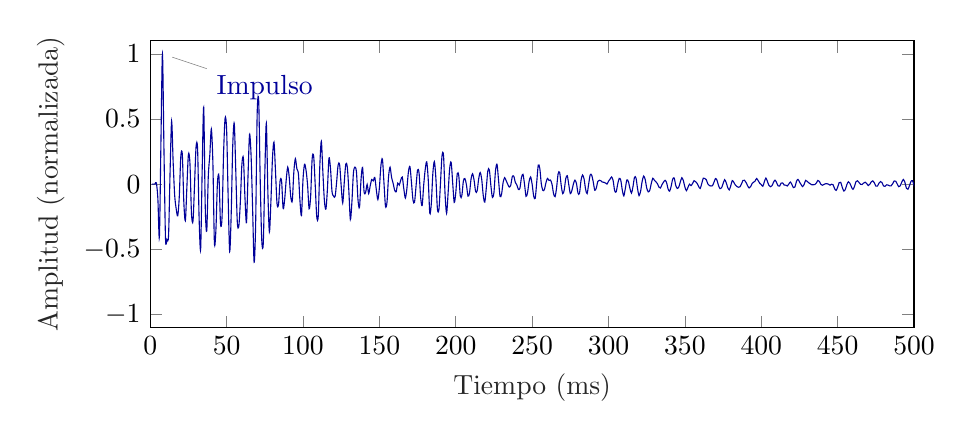
\begin{tikzpicture}

\begin{axis}[%
width=0.8\textwidth,
height=0.3\textwidth,
at={(0\textwidth,0\textwidth)},
scale only axis,
xmin=0,
xmax=500,
xlabel style={font=\color{white!15!black}},
xlabel={Tiempo (ms)},
ymin=-1.1,
ymax=1.1,
ylabel style={font=\color{white!15!black}},
ylabel={Amplitud (normalizada)},
axis background/.style={fill=white},
legend style={legend cell align=left, align=left, draw=white!15!black}
]
\addplot [color=black!40!blue, smooth]
  table[row sep=crcr]{%
1	4.2434738134034e-05\\
2	-0.000305107333076649\\
3	-7.00303905887267e-05\\
4	0.0102163738390573\\
5	-0.112658317720332\\
6	-0.406324005259592\\
7	0.31944440485853\\
8	1\\
9	0.254143471158102\\
10	-0.419421552342101\\
11	-0.426049295861048\\
12	-0.391400555358473\\
13	0.0981040777945736\\
14	0.483833119630901\\
15	0.168320936215935\\
16	-0.0859970762599573\\
17	-0.190508299724286\\
18	-0.243018733499582\\
19	-0.0987719084795913\\
20	0.210747821340874\\
21	0.227070515693981\\
22	-0.141382759360567\\
23	-0.280890280339065\\
24	-0.0190941612947313\\
25	0.229452560179539\\
26	0.158762720075231\\
27	-0.226287102827428\\
28	-0.282467801318148\\
29	-0.00503940027795124\\
30	0.287091012549922\\
31	0.269219668431788\\
32	-0.263795015217624\\
33	-0.499225118077277\\
34	0.105422543579266\\
35	0.589718130115671\\
36	-0.168493735741663\\
37	-0.359430073266253\\
38	0.0594348920738526\\
39	0.222884163049741\\
40	0.423905565786697\\
41	0.169746475134616\\
42	-0.448428448844936\\
43	-0.349434729393238\\
44	0.0100225795323468\\
45	0.0560272364984939\\
46	-0.303099856773429\\
47	-0.253889564060103\\
48	0.23234192057231\\
49	0.505904690192608\\
50	0.418494778447894\\
51	-0.0954006723407019\\
52	-0.517671052265655\\
53	-0.229571714919757\\
54	0.291956986380569\\
55	0.465429827611331\\
56	0.101402533289217\\
57	-0.293070159868023\\
58	-0.321418086440985\\
59	-0.133090839518047\\
60	0.151731987301162\\
61	0.197543487685493\\
62	-0.10130285321253\\
63	-0.29479540559754\\
64	0.0604133027735543\\
65	0.380137476085054\\
66	0.223202331101447\\
67	-0.179516539250699\\
68	-0.599675232169716\\
69	-0.307284551693044\\
70	0.540141287740539\\
71	0.640677984843933\\
72	0.0264150876811868\\
73	-0.429267349915847\\
74	-0.454558141731809\\
75	0.0755832132248315\\
76	0.466891775170438\\
77	-0.0590980872991054\\
78	-0.367175145091721\\
79	-0.131366219661402\\
80	0.194727338775749\\
81	0.322162139497323\\
82	0.098608302574462\\
83	-0.149886334811868\\
84	-0.154196905265678\\
85	0.0248283318823042\\
86	0.021645678888035\\
87	-0.187116275132325\\
88	-0.11650518990632\\
89	0.0310209873227905\\
90	0.130955914545893\\
91	0.0517600836509473\\
92	-0.0981347924997635\\
93	-0.126372322478858\\
94	0.0925800218392396\\
95	0.194798953188524\\
96	0.117775174148505\\
97	0.0783790449436879\\
98	-0.1251269770504\\
99	-0.240832472672594\\
100	0.035454599574507\\
101	0.152797575955049\\
102	0.105299456113073\\
103	-0.00706682739468079\\
104	-0.189611018476398\\
105	-0.0944133180597078\\
106	0.196586191451445\\
107	0.211804747862686\\
108	-0.00667469430374013\\
109	-0.249825265577499\\
110	-0.242687347408605\\
111	0.136721513472651\\
112	0.328828153139852\\
113	0.0944185448216786\\
114	-0.126003221017186\\
115	-0.191112373988062\\
116	-0.0350411528050927\\
117	0.199966879759643\\
118	0.119847114658569\\
119	-0.0572502811593267\\
120	-0.0910512073435825\\
121	-0.0958444684911797\\
122	0.0133702644259301\\
123	0.148101897439403\\
124	0.146651979151102\\
125	-0.0132571261748922\\
126	-0.144932274189273\\
127	0.010654652132871\\
128	0.153178028330387\\
129	0.130978914609784\\
130	-0.0476576428244471\\
131	-0.270963245458972\\
132	-0.140528094680974\\
133	0.0853112454921074\\
134	0.130835545676177\\
135	0.0924931284478134\\
136	-0.120051587045339\\
137	-0.177102480678457\\
138	0.0371928058235653\\
139	0.127959609110803\\
140	-0.0599990574245908\\
141	-0.0627313888408594\\
142	-0.00212402937717115\\
143	-0.0721876160693569\\
144	-0.0124906252990513\\
145	0.0360094308679209\\
146	0.0252631431896475\\
147	0.0518191336979612\\
148	-0.0437834827953338\\
149	-0.117981632034684\\
150	-0.0292763853273641\\
151	0.142005632885457\\
152	0.191068427242101\\
153	0.0103488200060156\\
154	-0.169699326082309\\
155	-0.137320382611392\\
156	0.0568251156432211\\
157	0.129417870705595\\
158	0.0506198407852594\\
159	0.00652463677499782\\
160	-0.0458751656890399\\
161	-0.0591677519568634\\
162	0.00738421650282817\\
163	-0.00703130163242349\\
164	0.0318282709056916\\
165	0.0543793011042908\\
166	-0.0362049096157193\\
167	-0.10651740675678\\
168	-0.0353479096588671\\
169	0.0942289376151848\\
170	0.134295257072552\\
171	0.0131625477971511\\
172	-0.121981508204044\\
173	-0.13952180224527\\
174	-0.0160694973783961\\
175	0.10877638555769\\
176	0.0832842033232737\\
177	-0.100431173229026\\
178	-0.164261877352033\\
179	-0.00954893336120222\\
180	0.112077588323132\\
181	0.171385583112794\\
182	0.0311299561038823\\
183	-0.222343604322589\\
184	-0.148974586548434\\
185	0.0824104242174712\\
186	0.172872288632277\\
187	0.042542604962307\\
188	-0.19106152633276\\
189	-0.192024428491607\\
190	0.0088846948834771\\
191	0.217461004554366\\
192	0.219072593677708\\
193	-0.0779842820162457\\
194	-0.223968732455035\\
195	-0.0664861343670395\\
196	0.118553378920581\\
197	0.166843463401449\\
198	0.00740557834018318\\
199	-0.14071526386698\\
200	-0.0671892564222389\\
201	0.0817634534168974\\
202	0.0617557646910996\\
203	-0.0930417383475515\\
204	-0.0865978131771499\\
205	0.0255189855460003\\
206	0.0431554407566068\\
207	-0.00604058857481959\\
208	-0.0918091074512972\\
209	-0.0682941217426674\\
210	0.0393914200984682\\
211	0.0791040166041626\\
212	0.030301662908073\\
213	-0.056136602907543\\
214	-0.0523983151060747\\
215	0.0409561999382504\\
216	0.0891191952794657\\
217	0.0365043645761034\\
218	-0.0875616848279606\\
219	-0.137852253356471\\
220	-0.0284548843452512\\
221	0.103078385620734\\
222	0.107949878982652\\
223	-0.0120350665206388\\
224	-0.102279367961046\\
225	-0.0635638457451932\\
226	0.100496370789642\\
227	0.15274070862705\\
228	0.0311269755749777\\
229	-0.0946517995159297\\
230	-0.0752682551755015\\
231	0.0128846884498444\\
232	0.0498888132935917\\
233	0.026360005551453\\
234	7.79022378196714e-05\\
235	-0.0223584443212985\\
236	-0.00766427103712886\\
237	0.0570655790829733\\
238	0.0601808020367116\\
239	0.0137279947801972\\
240	-0.00673958175144662\\
241	-0.0403883228201494\\
242	-0.031348045933953\\
243	0.0503081724390881\\
244	0.0754672687799598\\
245	0.00087901105786159\\
246	-0.0938608516431714\\
247	-0.0644502895835899\\
248	0.0201143367866052\\
249	0.0550681791359011\\
250	-0.000619648405461248\\
251	-0.0909182481454422\\
252	-0.109153313949321\\
253	0.0137708880162108\\
254	0.145882386525614\\
255	0.122049615755884\\
256	0.00266680473629322\\
257	-0.0477137107558292\\
258	-0.0419497184457214\\
259	0.00873475663888712\\
260	0.0437470401822679\\
261	0.0289364715410443\\
262	0.03151162024011\\
263	-0.000538120093835914\\
264	-0.0719918758077256\\
265	-0.0964718927539252\\
266	-0.0274812659419013\\
267	0.0794381606846173\\
268	0.0902784969155732\\
269	-0.00619325750631106\\
270	-0.0728387356438702\\
271	-0.0452518729547364\\
272	0.0415065693133556\\
273	0.0647258425048562\\
274	-0.00500829681197956\\
275	-0.0725999222960354\\
276	-0.0497784352866688\\
277	0.000752310835082426\\
278	0.0307166094751778\\
279	0.00608676545988374\\
280	-0.0681502048426523\\
281	-0.0700930929307333\\
282	0.029321406867723\\
283	0.0706052350790287\\
284	0.0393160388475735\\
285	-0.0401512793812913\\
286	-0.0724919350228106\\
287	0.00136660403484257\\
288	0.0712012199193168\\
289	0.0688434313006496\\
290	0.0172088426002119\\
291	-0.0469553445916517\\
292	-0.029606205441894\\
293	0.021024349888819\\
294	0.0297822344522842\\
295	0.0258182686042119\\
296	0.015424765639068\\
297	0.014596340932826\\
298	0.00854085178730202\\
299	0.000487765415982722\\
300	0.0228182881962766\\
301	0.0384994666932243\\
302	0.0552011899724789\\
303	0.0285647467799208\\
304	-0.049585522189318\\
305	-0.0596867280301012\\
306	0.000432778744880125\\
307	0.0445485189810029\\
308	0.0309135697626743\\
309	-0.0447182628378187\\
310	-0.090275082360165\\
311	-0.0331579162024127\\
312	0.0323299779940953\\
313	0.0196934447252488\\
314	-0.0316931331243495\\
315	-0.0688494380389102\\
316	-0.0200748759817202\\
317	0.052034527963599\\
318	0.0469639463611315\\
319	-0.0351958955350824\\
320	-0.0880734492340025\\
321	-0.0549242532201788\\
322	0.0202141360426822\\
323	0.0622289245903858\\
324	0.0358012238015704\\
325	-0.029819710380707\\
326	-0.0594779626476338\\
327	-0.0468180682967727\\
328	0.00577341752273242\\
329	0.0454326824394684\\
330	0.0304994112390773\\
331	0.0181471727007079\\
332	0.00415997360016718\\
333	-0.0230774475172097\\
334	-0.0301258992751627\\
335	-0.00351817480367345\\
336	0.0154935559578462\\
337	0.0293805509508047\\
338	0.0113993348299459\\
339	-0.037433231509965\\
340	-0.0539008479468635\\
341	-0.0161484505050566\\
342	0.0379783335305319\\
343	0.046785150784217\\
344	-0.00953691376133747\\
345	-0.0330822481678297\\
346	-0.0217303835157736\\
347	0.0172780419010792\\
348	0.0489747692393507\\
349	0.0265602932822162\\
350	-0.0225584975509037\\
351	-0.0501717989228041\\
352	-0.0247803080171138\\
353	-0.000209979310739072\\
354	-0.0111520710445348\\
355	0.00512303188395435\\
356	0.0264969893882494\\
357	0.0194849907384764\\
358	0.00548351648365042\\
359	-0.0177614956663774\\
360	-0.0332959888409619\\
361	0.00334742723680392\\
362	0.0452125599201167\\
363	0.0445468702614562\\
364	0.0336247824390057\\
365	0.00236398909515856\\
366	-0.0108177590376499\\
367	-0.0144012044676174\\
368	-0.012004745096533\\
369	0.0132066533295756\\
370	0.0429041146734335\\
371	0.0302277118415759\\
372	-0.0104773394855897\\
373	-0.0344542568789734\\
374	-0.0283710367054937\\
375	0.00400111953985061\\
376	0.034041053394958\\
377	0.0123562573841696\\
378	-0.0248798930180101\\
379	-0.0443324328667245\\
380	-0.0127007652255884\\
381	0.0274987306607954\\
382	0.0142068308153398\\
383	-0.00674589324421504\\
384	-0.0178977607682214\\
385	-0.0236760189014262\\
386	-0.0208664813910673\\
387	0.000318765237182106\\
388	0.0280427069447455\\
389	0.0298899829273864\\
390	0.0135987779480615\\
391	-0.0113421737564749\\
392	-0.0292236855831334\\
393	-0.0196050863545452\\
394	0.00513004241508952\\
395	0.0152305783949487\\
396	0.0241923885324127\\
397	0.0430875755562283\\
399	0.00650351434666163\\
400	-0.00390418419073058\\
401	-0.0163808607109104\\
402	0.0179660765792278\\
403	0.0468076039156244\\
404	0.0215092558023571\\
405	-0.00962535935826736\\
406	-0.019784575810661\\
407	-0.0124071416098559\\
408	0.0140352926419496\\
409	0.0304130267627443\\
410	0.012113601805936\\
411	-0.0134811746702894\\
412	-0.0145640678023824\\
413	0.00781262337699218\\
414	0.0093014204472297\\
415	-0.0067624452000814\\
416	-0.00745235216993478\\
417	-0.0143150791455469\\
418	0.00021101377302557\\
419	0.0164046855479683\\
420	-0.00158481591853388\\
421	-0.0264223996583155\\
422	-0.0225696346008135\\
423	0.0195210931047427\\
424	0.036884017318016\\
425	0.0169647835085129\\
426	-0.0019110640969302\\
427	-0.0185311580900702\\
428	-0.00363193338785095\\
429	0.02889931526704\\
430	0.0223407891387524\\
431	0.0112897203297848\\
433	-0.00441399808357801\\
434	-0.00468176819299515\\
435	-0.00311968028154297\\
436	0.00758816342113278\\
437	0.0281175924312151\\
438	0.0211610488794349\\
439	-0.000960052333766725\\
440	-0.00879715557852023\\
441	-0.00235846747290225\\
442	0.00282371777643675\\
443	0.00376019462129307\\
444	-0.000503929943477033\\
445	-0.00782279681783393\\
446	-0.000737570513990704\\
447	-0.00475165581065085\\
448	-0.0347967952396289\\
449	-0.0481855300386655\\
450	-0.0228921351777558\\
451	0.0116004779522996\\
452	0.0141549879012928\\
453	-0.0240395930988484\\
454	-0.0527800368865883\\
455	-0.0404179472573674\\
456	-0.00434876993614353\\
457	0.0180017840324922\\
458	0.00691907349289522\\
459	-0.021053907509895\\
460	-0.0398426040100048\\
461	-0.0178982621434329\\
462	0.0201176878541673\\
463	0.0258475057381133\\
465	-0.00176443867593434\\
466	-0.00247937028404976\\
467	0.00824667609805374\\
468	0.014986121715026\\
469	0.00427453796714872\\
470	-0.0105766838909176\\
471	-0.00149741030219275\\
472	0.017347225648507\\
473	0.0251093065790542\\
474	0.0110516863589964\\
475	-0.0155704175779761\\
476	-0.0152816398357345\\
477	0.0064252181913389\\
478	0.0195429751263418\\
479	0.0130065196967166\\
480	-0.0136514029958335\\
481	-0.017260731840679\\
482	-0.00500913717536378\\
483	-0.00696824345953928\\
484	-0.0129316154050798\\
485	-0.0130602274383023\\
486	0.00336729786306478\\
487	0.0243823891437955\\
488	0.0223730838646929\\
489	0.00112983178507875\\
490	-0.0195751815114136\\
491	-0.0128517940416941\\
492	0.0168775608927376\\
493	0.0360479266161633\\
494	0.0140244759079451\\
495	-0.0315260872309864\\
496	-0.0394578507611527\\
497	-0.0115326535533882\\
498	0.0206041748820098\\
499	0.026745505363408\\
500	-0.00948803025585221\\
501	-0.0346936412250898\\
};
\addplot[mark=none, color=black!40!blue] coordinates {(8,1)} node[pin=-15:{Impulso}]{} ;

\end{axis}
\end{tikzpicture}%
    }
    \caption{Respuesta al impulso de un sistema.}
    \label{graf:impulso}
\end{figure}





